\documentclass[12pt]{article}
% Paragraphs: no indent and a visible blank space between them (Wesley, 10 Oct). The parskip package
% sets both and keeps lists and headings consistent with the gap.
\usepackage[skip=12pt plus 2pt minus 1pt]{parskip}
\usepackage[a4paper, margin=1in]{geometry}
\usepackage{graphicx}
\usepackage{pgfgantt}
\usepackage{booktabs}
\usepackage{mathtools}
\usepackage{float}
\usepackage{caption}
\usepackage{tabularx}
\usepackage{ulem} 
\usepackage{titlesec}
\usepackage{siunitx}
\usepackage{listings}
\usepackage{xcolor}
\usepackage{nomencl}
\definecolor{darkblue}{rgb}{0.0,0.0,0.55}
% \redo{...}: marks a result that was flown before the rig twin and has to be flown again on it.
% The old text stays under each box as comments. List of what to fly: docs/redo_on_twin.md (code repository).
\definecolor{redoframe}{rgb}{0.80,0.40,0.00}
\definecolor{redoback}{rgb}{1.00,0.95,0.85}
\makeatletter
\newcommand{\redo}[1]{\if@noskipsec\leavevmode\fi\par\smallskip\noindent
  \fcolorbox{redoframe}{redoback}{\parbox{\dimexpr\linewidth-2\fboxsep-2\fboxrule\relax}{\small\raggedright
  \textbf{To re-fly on the rig twin:} #1}}\par\smallskip}
\makeatother
% \pendingfig{label}{caption}{run that fills it}: a figure whose data is not flown yet. The caption and
% label are final, so the text can cite it now; the box says which run fills it.
\newcommand{\pendingfig}[3]{%
  \begin{figure}[htbp]
  \centering
  \fcolorbox{redoframe}{redoback}{\parbox[c][0.32\textwidth][c]{\dimexpr\linewidth-2\fboxsep-2\fboxrule\relax}{%
    \centering\small\textbf{Pending:} #3}}%
  \caption{#2}\label{#1}
  \end{figure}}
\usepackage{amsfonts}
\usepackage{tikz}
\usetikzlibrary{angles, quotes, decorations.pathreplacing, shapes.geometric, arrows.meta, positioning, backgrounds, fit}
\usepackage{pgfplots}
\pgfplotsset{compat=1.18}
\usepackage[backend=biber,style=ieee]{biblatex}
\addbibresource{references.bib}
\addbibresource{references_extra.bib}
\usepackage{url}
\usepackage{microtype}
\setlength{\emergencystretch}{5em}
\tolerance=2000
\hbadness=2000
\usepackage[colorlinks=true,
            linkcolor=darkblue,
            urlcolor=darkblue,
            citecolor=blue,
            pdfborder={0 0 0}]{hyperref}
\usepackage{setspace}
\onehalfspacing
\usepackage{enumitem}
\setlist[itemize]{itemsep=-4pt}
\setlist[enumerate]{itemsep=-4pt}
% Float placement (9 Oct, page trim): let a large figure share a page with text instead of sitting
% alone, half empty, on a float page.
\renewcommand{\topfraction}{0.9}
\renewcommand{\bottomfraction}{0.8}
\renewcommand{\textfraction}{0.07}
\renewcommand{\floatpagefraction}{0.8}
\setcounter{topnumber}{3}
\setcounter{totalnumber}{4}

\makenomenclature
\renewcommand{\nompreamble}{(The nomenclature must respect the following order: latin symbols, Greek symbols, acronyms. Within each category of symbols, follow alphabetic order. An example is provided below)}

\begin{document}

\begin{titlepage}
\begin{center}

\includegraphics[width=6cm]{Images/UNSW.jpg}\\[1.3cm]
{\Large School of Mechanical and Manufacturing Engineering}\\[0.3cm]
{\Large Faculty of Engineering}\\[0.3cm]
{\Large UNSW Sydney}
\vfill
\vspace{1em}
\rule{0.7\linewidth}{0.4pt}\\[1em]
{\Large Wesley Donald} \\
\rule{0.7\linewidth}{0.4pt}\\[1.5em]
\vfill
{\LARGE\bfseries Mid--Flight Reconfiguration for Cooperative \\
\vspace{0.2cm}
Quadcopter Payload Transport}
\vfill
{\Large Thesis submitted as a requirement for the degree of\\
\vspace{0.2cm}
Bachelor of Engineering in Mechatronic Engineering}
\vfill
\large
\begin{tabularx}{\textwidth}{
  | >{\raggedright\arraybackslash}X
  | >{\raggedright\arraybackslash}X | }
\hline
Submitted: 20/11/26 & Student zID: z5600603 \\
\hline
Supervisor: Dr Mohammad Deghat & Co-Supervisor: Mitchell Torok \\
\hline
\end{tabularx}
\end{center}
\end{titlepage}

% ---- Front matter: roman numerals ----
\pagenumbering{roman}

% Originality statement
\textbf{ORIGINALITY STATEMENT} \\

\textit{`I hereby declare that this submission is my own work and to the best of my knowledge it contains no materials previously published or written by another person, or substantial proportions of material which have been accepted for the award of any other degree or diploma at UNSW or any other educational institution, except where due acknowledgement is made in the thesis. Any contribution made to the research by others, with whom I have worked at UNSW or elsewhere, is explicitly acknowledged in the thesis. I also declare that the intellectual content of this thesis is the product of my own work, except to the extent that assistance from others in the project's design and conception or in style, presentation and linguistic expression is acknowledged.'} \\

Signed: \raisebox{-0.3\height}{
\includegraphics[width=2cm]{Images/signature.png}} \\
Date: \hspace{0.1cm} \uline{20/11/26}

\newpage
\section*{Abstract}
\addcontentsline{toc}{section}{Abstract}
% Template: a short abstract restating the main objectives, the main findings and their significance;
% at most 100 words. The report is at most 50 pages, excluding appendices, bibliography, cover sheet,
% abstract, acknowledgements, nomenclature, contents and lists of figures and tables.
% DRAFT 4 Oct 2026 (about 100 words); update the findings once the hardware reconfiguration is flown.
% 10 Oct: the rig findings brought up to 8 Oct (four UAVs on the paths, Table tab:rig_oct7; four detaches,
% Table tab:rig_oct8; twin detach back in band in 0.9-1.0 s, Table tab:detach). Was: "In simulation this
% kept a 0.86 kg ring level through a detach. On hardware, three UAVs carried the ring to 1.0 m."
Cooperative transport of a cable-suspended payload by several UAVs usually assumes a fixed team.
This thesis investigates whether a centralised controller can keep the payload stable while UAVs leave
and join mid-flight. A load--cable model predictive planner with per-UAV tracking was built for
Betaflight UAVs. A detach or an attach resizes the planner's optimal control problem,
with the attachment geometry as a runtime parameter. On hardware, four UAVs carried a 0.86\,kg ring
within 3\,cm of its path on average, and three held it through four detaches, announced and
unannounced; in simulation the ring settled within a second of a detach.

% 11 Oct: the abstract is rewritten from docs/thesis_plan_2026-10-11.md section 8 once the join numbers are in
% (Fri 16 twin claim, 21-22 Oct rig); the network comparison is out of the abstract (Appendix F).
% --- original text, flown before the rig twin; kept to refill this place:
% with the attachment geometry as a runtime parameter. In simulation this kept a 0.86\,kg ring level
% through a detach and rejoined a UAV with under 2$^\circ$ of payload tilt, outperforming a dissipative
% alternative. On hardware, three UAVs carried the ring to 1.0\,m.

\newpage
\section*{Acknowledgments}
\addcontentsline{toc}{section}{Acknowledgments}
Mitch, Te-Jen, Mohammad.

\newpage
\tableofcontents

\newpage
\addcontentsline{toc}{section}{List of Figures}
\listoffigures

\newpage

\addcontentsline{toc}{section}{List of Tables}
\listoftables

\newpage

\addcontentsline{toc}{section}{Nomenclature}

% The nomenclature section is created here (variables and definitions can be edited below).
\nomenclature[1A]{\(A\)}{amplitude of …}
\nomenclature[1Cp]{\(C_p\)}{…}
\nomenclature[1D]{\(D\)}{…}
\nomenclature[1alpha]{\(\alpha\)}{…}
\nomenclature[2TLA]{\(TLA\)}{…}

\printnomenclature

\newpage
\pagenumbering{arabic}

\section{Introduction}

A drone or Unmanned Aerial Vehicle (UAV), is an aircraft that is operated without an onboard pilot, controlled either autonomously or through remote control. A quadcopter is a type of UAV with four horizontal rotors and is naturally underactuated, having four control inputs but six degrees of freedom \cite{kotaruDifferentialflatnessControlQuadrotors2018}; in this thesis, UAV means a quadcopter. Such UAVs have experienced significant growth in popularity since the development of low-cost microcontrollers and sensors, transitioning from hobbyist and videography uses to a variety of applications \cite{kardaszDronesPossibilitiesTheir2016}. They are agile, able to perform vertical takeoff and landing, and have the capacity to operate in confined or GPS-denied environments. This makes them attractive across a range of commercial applications, including package delivery, search and rescue, construction, and agriculture \cite{olleroPresentFutureAerial2022}. In many of these contexts, the ability to carry a payload is essential, for example, to deliver a package, transport construction materials, or recover an object in a search and rescue mission \cite{thusooQUADROTORSPRESENTERA2021, choiOverviewDroneApplications2023}. Consequently, the problem of UAV payload transport has received significant research attention over the past two decades. \\

Despite these advantages, these UAVs have notable limitations. Their thrust-to-weight ratio constrains the maximum payload they can carry, and a suspended load introduces pendulum-like swing dynamics that can destabilise the vehicle and consume significant control effort to reject \cite{geronelDynamicResponsesDue2023}. These limitations have motivated research into cooperative multi-UAV payload transport, where multiple UAVs jointly lift a single load \cite{Carney_2022}. This approach offers several advantages over single-UAV systems: it increases the total liftable payload mass, reduces oscillation by constraining the load through multiple attachment points, can enable full six-degree-of-freedom control of the payload pose, and avoids the cost and complexity of constructing a single large-scale vehicle \cite{tudelft, mohammadiDecentralizedMotionControl2018}. \\

A common method to attach the payload to the UAVs is through flexible cables. Compared to rigid attachments, cables are mechanically simpler and safer in the event of a collision. However, they introduce additional challenges as cable tension must remain positive to remain taut and in multi-UAV systems, the tension contributed by each UAV must be carefully allocated to avoid overloading any single vehicle. Formation constraints and inter-UAV collision avoidance further complicate the control problem \cite{kotaruDynamicsControlQuadrotor2017}. \\

This field has been explored extensively, with a large body of work addressing trajectory tracking, formation control, tension allocation, and disturbance rejection for fixed-team systems \cite{wangRobustCooperativeTransportation2024, gimenezMultiobjectiveControlCooperative2018, wahbaKinodynamicMotionPlanning2024}. Most existing work is validated in simulation, with fewer papers demonstrating real-world experimental results and very few conducting outdoor experiments, despite the intended applications being predominantly outdoors \cite{estevezReviewAerialTransportation2024}. \\

While robustness to disturbances such as wind and payload uncertainty is frequently addressed, less attention has been given to changes in team composition during a mission. Several works consider reducing the number of active UAVs, such as \cite{tensionbased, quan2025swarm}, however to the author's knowledge, no existing work has demonstrated the dynamic addition of a UAV to an active system in either simulation or real-world experiments. This problem presents several technical challenges as the joining UAV must accurately localise the payload attachment point and load distribution must be reallocated smoothly across the team. Additionally, the existing system must remain stable during the joining transient. \\

The ability to dynamically add UAVs to an active transport mission would offer significant practical benefits. In real-world deployments, a UAV may need to leave the formation due to low battery, mechanical failure, or mission reassignment, reducing the team's total lift capacity and potentially compromising the mission \cite{farrasFaultTolerantControlMultiQuadcopter2024}. If a replacement UAV could join the system mid-flight, the mission could continue uninterrupted without requiring the entire team to land and restart. Dynamic addition could also enable more flexible mission profiles, for example, a lighter team could carry the payload through a narrow passage or constrained environment, with additional UAVs joining once the passage is cleared to increase stability and carrying capacity for the remainder of the mission, with passage navigation being explored in several works \cite{tudelft, tensionbased}. \\

Furthermore, starting a mission with a minimal number of UAVs and adding more as needed reduces unnecessary energy consumption during phases where full team capacity is not required. Taken together, these scenarios highlight that the dynamic addition of UAVs is both a robustness feature and a capability that could meaningfully expand the operational envelope of cooperative aerial transport systems. This process is summarised in Figure~\ref{fig:mission_profile}. \\

\tikzset{
  block/.style={
    rectangle, rounded corners=4pt,
    minimum width=5.3cm, minimum height=0.85cm,
    draw, thick, align=center,
    font=\small
  },
  transport/.style={block, fill=blue!6, draw=blue!40},
  event/.style={block, fill=orange!12, draw=orange!60},
  docking/.style={block, fill=purple!8, draw=purple!45},
  arrow/.style={-Stealth, thick},
  phase/.style={font=\footnotesize\color{gray}}
}

\begin{figure}[h]
\centering
\begin{tikzpicture}[node distance=0.6cm and 1.2cm]

\node (p1) [transport]
{\textbf{Initial transport}\\[-2pt]\scriptsize $N$ UAVs follow the planned trajectory};

\node (ev) [event, below=of p1]
{\textbf{UAV departure}\\[-2pt]\scriptsize failure / low battery};

\node (p2) [transport, below=of ev]
{\textbf{Reduced team}\\[-2pt]\scriptsize $N\!-\!1$ UAVs maintain stability};

\node[phase, left=0.4cm of p1] {Phase 1};
\node[phase, left=0.4cm of ev] {Phase 2};
\node[phase, left=0.4cm of p2] {Phase 3};

\draw[arrow] (p1) -- (ev);
\draw[arrow] (ev) -- (p2);

\node (p3) [docking, right=1.2cm of p1]
{\textbf{Replacement approach}\\[-2pt]\scriptsize localises docking point};

\node (p4) [docking, below=of p3]
{\textbf{Attachment}\\[-2pt]\scriptsize guided electromagnetic docking};

\node (p5) [transport, below=of p4]
{\textbf{Full team resumes}\\[-2pt]\scriptsize load redistributed to $N$ UAVs};

\node[phase, right=0.4cm of p3] {Phase 4};
\node[phase, right=0.4cm of p4] {Phase 5};
\node[phase, right=0.4cm of p5] {Phase 6};

\draw[arrow] (p3) -- (p4);
\draw[arrow] (p4) -- (p5);

\draw[arrow, thick] (p2.east) -- ++(0.8,0) |- (p3.west);

\end{tikzpicture}

\caption{Mission profile for dynamic UAV replacement during transport.}
\label{fig:mission_profile}
\end{figure}

This thesis focuses specifically on the multi-UAV control problem associated with maintaining stable payload transport following mid-mission UAV addition, corresponding to Phases 2, 4, and 6 in Figure~\ref{fig:mission_profile}. A complementary component of the overall system, the physical docking and attachment mechanism during Phases 4 and 5 is developed by a collaborating student. \\

Accordingly, the present contribution is focused on post-attachment system integration, including redistribution of cable forces, re-stabilisation of the formation, and recovery of coordinated transport performance. Validation is in simulation and on a hardware rig.
% contributions.tex -- research questions and contributions (draft 4 Oct 2026). Follows the
% introduction. The research questions are those of the project plan; the contributions list
% what has been built and shown so far, and is to be trimmed to what the final results support.

\subsection{Research Questions}
\label{sec:rq}

The research question of this thesis is whether a centralised controller can manage the join and
leave transients of individual agents in a multi-UAV payload system while keeping the payload
stable. Two questions follow from it.
\begin{enumerate}[label=\textbf{RQ\arabic*}]
    \item Can a centralised planner that has the whole team's state redistribute the load when a UAV
    leaves the payload and when a new UAV attaches to it mid-flight, with a transient small enough
    for the transport to continue?
    \item Does a decentralised dissipative control law \cite{quan2025swarm} or a trajectory-based
    optimal control approach \cite{tudelft} better balance robustness and tracking performance
    for this problem?
\end{enumerate}
The working hypothesis is that the centralised approach suits a change of team composition,
because the coordinating node can recompute the force distribution for the new team at the moment
of the event, rather than relying on the remaining agents to absorb it passively.

\subsection{Contributions}
\label{sec:contributions}

The work to date contributes the following.
\begin{enumerate}
    \item \textbf{A centralised payload controller flown on commercial-grade hardware.} The
    load--cable planner of \cite{tudelft} is combined with a cable-aware tracking MPC per UAV that
    commands Betaflight flight controllers over their radio links, with no changes to the
    UAVs' firmware. It includes a floor start for rigid rods, a pretension and lift procedure, and
    a thrust map identified on the rig (Sections~\ref{sec:controller} and~\ref{sec:takeoff}).
    \item \textbf{Reconfiguration by resizing the optimal control problem.} The attachment
    geometry is a runtime parameter of the planner, so a detach or an attach becomes a switch to
    a pre-built solver for the new team size, with each UAV kept on its real attachment point
    (Section~\ref{sec:reconfig}).
    \redo{OCP resize against handing the payload to a dissipative network during the transient, on a detach and on an attach.}
% --- original text, flown before the rig twin; kept to refill this place:
%     (Section~\ref{sec:reconfig}). In simulation this outperforms handing the payload to a
%     dissipative network during the transient.
    \item \textbf{A geometric condition for a level detach.} Whether the payload can stay level
    after a UAV leaves depends on whether its centre of mass stays inside the polygon of the
    surviving attachment points. This sets the attachment layout for four UAVs.
    \item \textbf{Mid-flight attachment of a new UAV.} A free UAV welds onto the carried payload
    through an electromagnet and is folded into the planner, in combination with a collaborator's
    approach controller.
    \redo{the full sequence in simulation: a UAV leaves, completes a pick-up task and rejoins while the team flies an orbit (the rejoin mission).}
% --- original text, flown before the rig twin; kept to refill this place:
%     approach controller. The full sequence (a UAV leaves, completes a pick-up task and rejoins
%     while the team flies an orbit) is demonstrated in simulation.
    \item \textbf{A comparison of the trajectory-based and dissipative approaches} on the same
    plant, tracker and test cases, including the tracking architecture the dissipative method
    assumes.
    \redo{the comparison itself (Section~\ref{sec:sim_architecture}).}
    \item \textbf{An analysis of steady errors in the cascade.} Several sources of steady payload
    error were identified and separated: a relaxed initial condition in the tracker, a breakaway
    pull cap held for the whole flight, model errors in thrust and rod mass, and external forces.
    Integral action in the planner's model and several estimation approaches from the
    literature are compared against them.
    \item \textbf{A simulation and verification environment that mirrors the rig.} A Gazebo twin
    of the lab set-up runs the same launch files and parameters as the hardware. Every run is
    recorded against a named baseline, with a set number of repeats.
    \item \textbf{Hardware results} with three UAVs carrying a 0.86\,kg ring: hover at up to
    1.0\,m, a circle and a figure-eight, and an account of the gap between simulation and the rig.
\end{enumerate}


\section{Literature Review}
\label{sec:lit}

% Template: develop from the previous reports and the supervisors' feedback; flow logically, not
% necessarily chronologically; end with the major work, its relevance, and the research gaps.
This section reviews the models used for multi-UAV cable-suspended transport, the centralised and
distributed control approaches, the work on changes in team composition, the execution layer and
steady-error rejection, and simulation fidelity, and ends with a comparison and the research gap
this thesis addresses.

% SUPERSEDED 12 Oct 2026: no longer input. Its content is condensed into lit_transport.tex (Section 2.1);
% fig:tension is not in the main text. Listed for deletion in docs/thesis_work_2026-10-12b.md.
% modelling.tex -- Literature review: cable models and their assumptions.
% Restructured 9 Oct (structure audit): the single-quadrotor model and fig:quad_frames are cut, the
% spring-damper equation is cut, and this thesis's own payload model moved to Source/src/model.tex
% (Methodology), merged with the planner's model. Simulation fidelity moved to Literature_review.tex.

\subsection{Cable-Suspended Transport and Model Assumptions}
\label{sec:lit_models}

The assumptions made about the cable set both the complexity of the dynamics and the validity of
the controller. The literature uses two models (Figure~\ref{fig:tension}).

\begin{figure}[h]
\centering
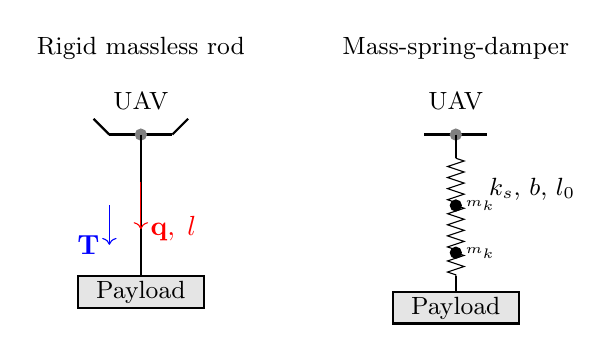
\begin{tikzpicture}[scale=1.0]
  % --- Left: Rigid rod ---
  \node[font=\small] at (-2, 3.5) {Rigid massless rod};

  % UAV
  \draw[thick] (-2.4,2.4) -- (-1.6,2.4);
  \draw[thick] (-2.4,2.4) -- (-2.6,2.6);
  \draw[thick] (-1.6,2.4) -- (-1.4,2.6);
  \filldraw[gray] (-2,2.4) circle (2pt);
  \node[above] at (-2,2.6) {\small UAV};

  % Rigid cable with unit vector label
  \draw[thick] (-2,2.4) -- (-2,0.6);
  \draw[->,red] (-2,1.8) -- (-2,1.2)
      node[right] {$\mathbf{q}, \; l$};

  % Payload
  \draw[thick,fill=gray!20] (-2.8,0.2) rectangle (-1.2,0.6);
  \node[font=\small] at (-2,0.4) {Payload};

  % Tension label
  \draw[->,blue] (-2.4,1.5) -- (-2.4,1.0)
      node[left] {$\mathbf{T}$};

  % --- Right: Spring-damper ---
  \node[font=\small] at (2, 3.5) {Mass-spring-damper};

  % UAV
  \draw[thick] (1.6,2.4) -- (2.4,2.4);
  \filldraw[gray] (2,2.4) circle (2pt);
  \node[above] at (2,2.6) {\small UAV};

  % Spring segments with lumped masses
  \draw[thick] (2,2.4) -- (2,2.1);
  \draw[decorate, decoration={zigzag,segment length=4pt, amplitude=3pt}]
      (2,2.1) -- (2,1.5);
  \filldraw (2,1.5) circle (2pt) node[right] {\tiny $m_k$};
  \draw[decorate, decoration={zigzag,segment length=4pt, amplitude=3pt}]
      (2,1.5) -- (2,0.9);
  \filldraw (2,0.9) circle (2pt) node[right] {\tiny $m_k$};
  \draw[decorate, decoration={zigzag,segment length=4pt, amplitude=3pt}]
      (2,0.9) -- (2,0.6);
  \draw[thick] (2,0.6) -- (2,0.4);

  % k_s and b labels
  \node[right, font=\small] at (2.3,1.7) {$k_s,\, b,\, l_0$};

  % Payload
  \draw[thick,fill=gray!20] (1.2,0.0) rectangle (2.8,0.4);
  \node[font=\small] at (2,0.2) {Payload};
\end{tikzpicture}
\caption{Cable modelling approaches.}
\label{fig:tension}
\end{figure}

The most common is the \textit{rigid massless rod}, adopted by \cite{efficient} and \cite{wahbaKinodynamicMotionPlanning2024}: a rigid link of fixed length $l$ along the unit vector $\mathbf{q}_i$, with the tension acting purely along it,

\begin{equation}
    \mathbf{T}_i = \lambda_i \mathbf{q}_i, \quad \lambda_i \geq 0
\end{equation}

where $\lambda_i$ is the tension, non-negative because a cable can pull but not push. The state stays compact and tractable, but slack cannot be captured.

The \textit{mass-spring-damper chain} of \cite{distributedNMPC} discretises the cable into $n$ lumped masses joined by spring--damper links of stiffness $k_s$, damping $b$ and rest length $l_0$. It captures sag and oscillation, at $6n$ extra states per cable.

Whatever the model, most controllers assume taut cables, with tension strictly positive throughout the task. A slack cable adds a unilateral constraint and a discontinuity in the equations of motion, and handling it rigorously remains open \cite{efficient}. For moderately aggressive indoor flight the rigid rod with taut cables is sufficient, consistent with \cite{tudelft}.

% control.tex -- Literature review: control architectures, changes in team composition, execution
% layer. Restructured 9 Oct (structure audit): existing.tex merged in (the TU Delft, Quan and Bacheti
% paragraphs), fig:cost_scaling cut, the RL and hybrid paragraphs cut to one sentence each, the stale
% architecture paragraph and fig:control_arch cut, the comparison moved to Literature_review.tex.

\subsection{Centralised Control}

Multi-UAV control architectures are typically classified according to their information structure and decision-making hierarchy, which directly affects scalability, robustness to communication failure, and computational burden \cite{nathanReviewAutonomousMultiagent2011}. Centralised architectures rely on a single coordinator that has global state information and computes all control actions. However, distributed and decentralised approaches allocate computation across UAVs, relying only on local communication or sensing. These differences are important in cable-suspended payload systems, where coupling through the payload induces strong dependencies between UAVs that must be either explicitly coordinated or implicitly handled through local interactions \cite{brambillaSwarmRoboticsReview2013}. Figure~\ref{fig:arch_comparison} highlights the difference in information flow and coordination structure between centralised and distributed implementations.

\begin{figure}[h]
\centering
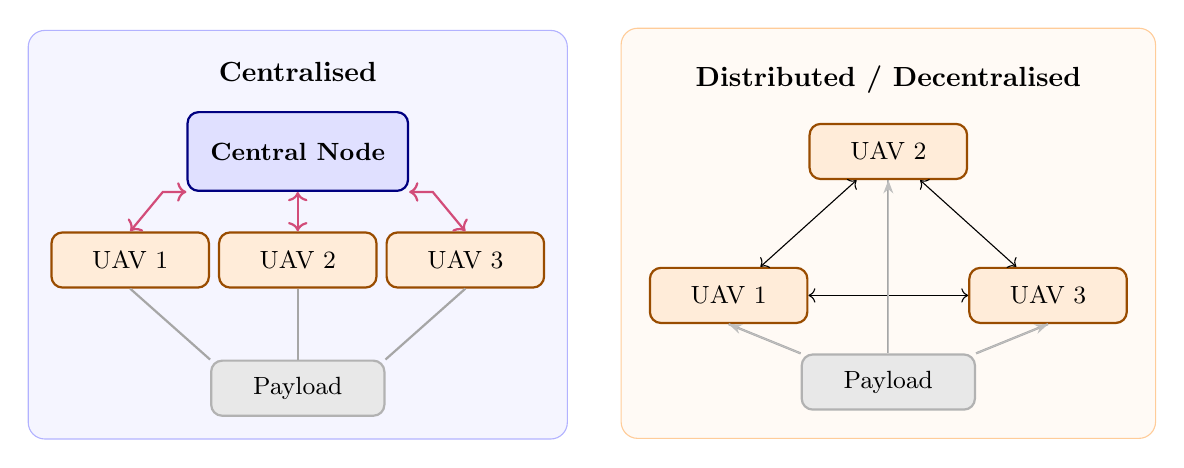
\begin{tikzpicture}[
    node distance = 0.55cm and 0.6cm,
    box/.style     = {rectangle, rounded corners=4pt, draw, thick,
                      minimum width=2.0cm, minimum height=0.7cm,
                      font=\small, text centered},
    central/.style = {box, fill=blue!12, draw=blue!50!black},
    uav/.style     = {box, fill=orange!15, draw=orange!60!black},
    payload/.style = {box, fill=gray!18, draw=gray!60, minimum width=2.2cm},
    arrow/.style   = {-Stealth, thick},
    dasharrow/.style = {-Stealth, thick, dashed, gray},
    label/.style   = {font=\footnotesize\itshape}
]

%% LEFT PANEL — CENTRALISED
\begin{scope}
\node[central, minimum width=2.8cm, minimum height=1.0cm]
    (coord) {\textbf{Central Node}};

\node[uav, below left=0.5cm and -0.3cm of coord]  (u1l) {UAV 1};
\node[uav, below=0.5cm of coord]                  (u2l) {UAV 2};
\node[uav, below right=0.5cm and -0.3cm of coord] (u3l) {UAV 3};
\node[payload, below=0.9cm of u2l] (pl) {Payload};

\draw[<->, thick, purple!70] (coord.south west) -- ++(-0.3,0) -- (u1l.north);
\draw[<->, thick, purple!70] (coord.south)      -- (u2l.north);
\draw[<->, thick, purple!70] (coord.south east) -- ++(0.3,0) -- (u3l.north);

\draw[thick, gray!70] (u1l.south) -- (pl.north west);
\draw[thick, gray!70] (u2l.south) -- (pl.north);
\draw[thick, gray!70] (u3l.south) -- (pl.north east);

\node[above=0.25cm of coord, font=\normalsize\bfseries] (ltitle) {Centralised};

\begin{scope}[on background layer]
  \node[draw=blue!30, fill=blue!4, rounded corners=6pt, inner sep=8pt,
        fit=(ltitle)(u1l)(u3l)(pl)] {};
\end{scope}
\end{scope}

%% RIGHT PANEL — DISTRIBUTED
\begin{scope}[xshift=7.5cm]
\node[uav] (u2r) {UAV 2};
\node[uav, below left=1.1cm and 0cm of u2r]  (u1r) {UAV 1};
\node[uav, below right=1.1cm and 0cm of u2r] (u3r) {UAV 3};
\node[payload, below=2.2cm of u2r] (pr) {Payload};

\draw[<->] (u1r) -- (u2r);
\draw[<->] (u2r) -- (u3r);
\draw[<->] (u1r) -- (u3r);

\draw[thick, gray!70] (u1r.south) -- (pr.north west);
\draw[thick, gray!70] (u2r.south) -- (pr.north);
\draw[thick, gray!70] (u3r.south) -- (pr.north east);

\draw[arrow, gray!50, thin] (pr.north west) -- (u1r.south);
\draw[arrow, gray!50, thin] (pr.north)      -- (u2r.south);
\draw[arrow, gray!50, thin] (pr.north east) -- (u3r.south);

\node[above=0.25cm of u2r, font=\normalsize\bfseries] (rtitle)
    {Distributed / Decentralised};

\begin{scope}[on background layer]
  \node[draw=orange!40, fill=orange!4, rounded corners=6pt, inner sep=10pt,
        fit=(rtitle)(u1r)(u2r)(u3r)(pr)] {};
\end{scope}
\end{scope}

\end{tikzpicture}
\caption{Centralised versus distributed/decentralised control architectures.}
\label{fig:arch_comparison}
\end{figure}

In a centralised architecture, a single node receives state information from all UAVs and computes commands for the entire team. This simplifies the enforcement of global constraints such as cable tension limits, collision avoidance between UAVs, and force allocation, and is a natural fit when a single computer commands all UAVs, as is the case in this work. The primary drawbacks are that computational cost tends to grow with the number of UAVs, and the central node means a single point of failure for the system \cite{dimakosStudyCentralisedDecentralised2021}.

\subsubsection{Trajectory-Based Planning with Receding Horizon}

Several centralised methods separate the control problem into a high-level trajectory planner and a low-level tracker. Sun et al.\ \cite{tudelft}, the closest prior work and the primary performance benchmark of this thesis, adopt this structure. A centralised receding-horizon optimal control problem is solved online at 10\,Hz over the full coupled load--cable--UAV dynamics, enforcing thrust limits, cable tautness and collision avoidance directly as path constraints, and generates trajectories for each UAV and the payload. Each UAV tracks its trajectory with an onboard incremental nonlinear dynamic inversion (INDI) controller that compensates for cable forces through inertial measurements, removing the need for any sensors on the load (Section~\ref{sec:lit_execution}). Real-world experiments with three and four UAVs reach speeds above 5\,m/s and accelerations above 8\,m/s\textsuperscript{2}, at least eight times the agility of prior force-based methods, including flight through narrow passages. The limitations are that the solve time grows exponentially with the number of UAVs, although the authors believe the approach can be scaled up with further optimisation, and that the framework assumes a fixed team throughout the mission. \\

The work in \cite{wahbaKinodynamicMotionPlanning2024} takes a hierarchical offline approach, using a sampling-based geometric planner to first find a feasible path through a cluttered environment, followed by constrained nonlinear trajectory optimisation enforcing full system dynamics, actuator limits, and collision avoidance. Formation changes are permitted so UAVs can reconfigure to pass through narrow gaps while maintaining payload stability, though the focus is on offline motion planning rather than real-time control.

\subsubsection{Nonlinear Model Predictive Control}

Nonlinear model predictive control (NMPC) solves a receding-horizon optimisation over the full nonlinear system dynamics at each timestep and represents the most constraint-rich centralised approach in the literature. Sun et al.\ \cite{sunNonlinearMPCFullPose2023} extend a centralised NMPC formulation to up to ten UAVs in simulation with solve times under 100\,ms, though the approach is untested on hardware beyond simulation. The primary limitation of centralised NMPC is that the solve time grows with the number of UAVs, as each additional UAV expands the state and decision variable dimensions of the optimisation problem, making real-time implementation increasingly difficult at scale. \\

A related approach is presented in \cite{liNonlinearModelPredictive2023}, where NMPC is used to manipulate a rigid-body payload with full six-degree-of-freedom pose control. In contrast to full-system formulations, the method exploits mechanical redundancy by parameterising the optimisation using only payload states on $\mathrm{SE}(3)$, rather than explicitly including all UAV states. This reduced-order representation lowers computational complexity while still capturing the essential coupled dynamics. The redundancy in the system is then leveraged to achieve secondary objectives such as separation between UAVs and obstacle avoidance, while respecting actuator limits and payload constraints. The approach is validated in both simulation and real-world experiments, demonstrating accurate payload tracking with improved computational efficiency relative to full-state NMPC formulations.

\subsubsection{Optimisation-Based Force Allocation}

A complementary method focuses on how to allocate cable tensions across the team given a desired payload wrench, treating allocation as a separable subproblem. The work in \cite{efficient} uses geometric control on $\text{SE}(3)$ to compute the required payload force and torque, then allocates tensions by solving a cascaded sequence of quadratic programs (QPs), yielding roughly quadratic rather than exponential scaling with the number of UAVs. Scalability to approximately ten robots is claimed, though experiments are demonstrated with up to three. The method assumes rigid massless cable rods and taut cables throughout. \\

A similar hierarchical structure is proposed by \cite{vazquez-soquiSQPBasedCableTensionAllocation2026}, where a sequential quadratic programming (SQP) optimiser allocates cable tensions at the lower level by minimising the sum of squared tensions while penalising cable misalignment. Simulation results with four UAVs show millisecond-level solve times, though the method has not been validated on hardware.

\subsubsection{Leader-Follower Control}

Leader-follower control assigns one UAV or the payload as the leader, with the remaining UAVs tracking desired offsets. Bacheti et al.\ \cite{tensionbased} treat the payload as the leader and each UAV as an independent follower. The resultant cable tension on the payload is a virtual control input, computed through feedback linearisation and distributed among the UAVs, each of which tracks the position and attitude references that realise its share of the cable force. This forms a hierarchical structure linking the load dynamics to each vehicle's actuation. Experiments show trajectory tracking and stable formation reconfiguration across several scenarios (Section~\ref{sec:lit_team}). The system relies on simplified modelling assumptions, including a point-mass payload and rigid, always-taut cables, and does not incorporate adaptive force redistribution under uncertainty. \cite{quan2025swarm} note that leader-follower approaches place high demands on robot homogeneity, and system performance degrades significantly when the leader fails. \\

A constrained centralised framework is proposed by \cite{9945662} using universal barrier functions to enforce both safety and performance constraints simultaneously, combined with adaptive estimators to handle actuator saturation and inertia uncertainty. This provides guarantees on constraint satisfaction even under model uncertainty, though the approach is validated in simulation only and does not consider dynamic team composition changes.

\subsubsection{Limitations of Centralised Approaches}

Across the centralised literature, three limitations recur consistently. First, computational cost scales with the number of UAVs, ranging from quadratic in the best case \cite{efficient} to exponential in NMPC and trajectory-based formulations \cite{tudelft}. Second, most centralised methods reviewed assume a fixed team throughout the mission, none explicitly handle a UAV joining mid-task, and few address dropout beyond passive tolerance. Third, the central node is a single point of failure. These limitations motivate the distributed and decentralised approaches reviewed next.

\subsection{Distributed and Decentralised Control}

Distributed and decentralised architectures avoid a central coordinator. In a decentralised system each UAV operates using only local sensor measurements with no communication to other UAVs. In a distributed system UAVs share information with neighbours through peer-to-peer communication to achieve a joint objective \cite{nathanReviewAutonomousMultiagent2011}. Both approaches generally offer better fault tolerance and scalability than centralised methods, though coordinating global objectives such as precise force allocation and six degree-of-freedom manipulation becomes more challenging \cite{scattoliniArchitecturesDistributedHierarchical2009}.

\subsubsection{Dissipative Control}

Energy-based dissipative control gives the most notable robustness to changes in the team. Quan et al.\ \cite{quan2025swarm} propose a fully decentralised dissipative controller inspired by table mechanics, in which each UAV independently damps the relative motion between itself and the payload, using only local measurements and no communication between UAVs. Any disturbance, from wind, cable perturbations or a UAV suddenly leaving the system, injects excess energy into the payload--swarm system, which the controller removes by computing damping forces proportional to relative velocity errors. Performance is further validated under varying UAV capabilities, cable length uncertainty and payload weight variation. The implementation depends on Differential GPS, limiting deployment to GPS-available outdoor environments. \\

The work in \cite{liuVirtualTubeBasedCooperativeTransport2026} extends the dissipative framework to a distributed setting by combining it with a virtual tube navigation concept, defining a corridor around the desired payload trajectory that the formation must remain inside. Cable tensions are allocated using dissipative systems theory, and the formation adapts to avoid obstacles while remaining within the tube. Simulations with up to ten UAVs and outdoor experiments demonstrate payload transport through constrained environments, though real-time tube generation remains future work.

\subsubsection{Distributed Model Predictive Control}

Several works distribute the MPC problem across UAVs to reduce the computational load on each. The work in \cite{distributedNMPC} assigns each UAV a subset of the global optimisation problem, solved locally and coordinated via a peer-to-peer network, with real-world experiments demonstrating centimetre-level position tracking. The authors identify keeping communication complexity independent of team size as a key open problem. \\

Centralised and decentralised linear MPC formulations are compared by \cite{DistributedMPC} in simulation for four UAVs. Both yield comparable tracking performance, but the decentralised formulation can run at a higher update frequency within the same compute budget. The linearised model improves tractability but decreases the ability for aggressive manoeuvres. \\

The work in \cite{tasoojiEventTriggeredNonlinearModel} reduces communication overhead further by updating the distributed NMPC only when the system deviates significantly from the planned trajectory, with the controller enforcing separation between robots and obstacle avoidance. This framework is extended in \cite{tasoojiCooperativeControlMultiQuadrotors}, which integrates global A* path planning with event-triggered NMPC for local control, alongside a decentralised communication architecture. The event-based update method, driven by perception inputs such as dynamic obstacle detection, improves responsiveness while reducing unnecessary computation.

\subsubsection{Sliding Mode Control}

A Distributed Fixed-Time Homogeneous Sliding Mode Control Protocol (DFHSMC) is proposed by \cite{DFHSMC} within a leader-follower structure, augmented with a disturbance observer. The controller minimises payload swing and demonstrates stability in three-UAV experiments under windy conditions, though it inherits the fragility of the leader-follower paradigm and does not address dynamic team changes. A three loop control structure is adopted by \cite{kotaruDynamicsControlQuadrotor2017} consisting of attitude control, sliding mode formation control driven by cable load states, and a payload navigation controller. Results are demonstrated in simulation only.

\subsubsection{Adaptive, Vision-Based, Learning and Hybrid Approaches}

A leaderless distributed nonlinear adaptive controller is proposed in \cite{arabPlanningDistributedControl2021} in which cable forces are modelled as an adaptive term, making the controller independent of payload dynamics. Path planning is handled by RRT*, and the adaptive term converges online. \\

The work in \cite{9376103} removes the dependence on external localisation entirely using onboard monocular cameras and inertial measurement units, with a distributed $\text{SE}(3)$ payload state estimator fusing local measurements via peer-to-peer communication. The case where payload mass and cable lengths are both unknown is addressed in \cite{10144367} using cable tension analysis and an admittance model with online parameter estimation. \\

Reinforcement learning has been used as a compensator for actuator saturation on top of a dynamic control allocation, in simulation only \cite{liMultiUAVCooperativeTransportation2021}, and multi-agent reinforcement learning is a promising but still fragmented paradigm for cooperative UAV control \cite{ekechiSurveyUAVControl2025}. Hybrid approaches combine centralised planning with distributed execution, for example a backstepping controller with a force distribution split into a payload position layer and a cable configuration layer \cite{wangRobustCooperativeTransportation2024}, a null-space formation controller for two UAVs \cite{gimenezMultiobjectiveControlCooperative2018}, and insetting-formation trajectory planning \cite{zhangIFBasedTrajectoryPlanning2023}.

\subsection{Changes in Team Composition}
\label{sec:lit_team}

Most of the work above assumes a fixed team \cite{efficient, wahbaKinodynamicMotionPlanning2024, quan2025swarm}; a few works let the team or its formation change during a mission, and none adds a UAV to a carried payload. \\

Quan et al.\ \cite{quan2025swarm} demonstrate experimentally robustness to a UAV dropping out mid-mission: the remaining UAVs self-organise and continue the trajectory with minimal payload swing, without replanning, a robustness rarely seen in the experimental literature. The critical limitation is that this robustness does not extend to addition, as a joining UAV receives no information about force sharing or attachment configuration, leaving the expansion of the team unaddressed. \\

Bacheti et al.\ \cite{tensionbased} handle removal explicitly: before a UAV releases, the remaining UAVs reposition to minimise the departure transient, which also lets the formation contract for narrow corridor traversal. Their leader-follower strategy reconfigures the formation during operation, with contraction and restoration of the formation shown experimentally. Although this approach is limited to reconfiguring the formation, the idea could be beneficial when adding or removing UAVs. The offline planner of \cite{wahbaKinodynamicMotionPlanning2024} likewise changes the formation, not the team, to pass through narrow gaps. \\

For joining, Tasooji et al.\ \cite{tasoojiCooperativeControlMultiQuadrotors} propose an event-triggered, decentralised architecture that suggests improved scalability through reduced communication and computation demands, but the ability to accommodate varying team sizes is not explicitly analysed, and the join protocol has neither experimental validation nor explicit force reallocation. What none of these provides is a force allocation that is recomputed for the new team at the moment a UAV leaves or joins.
% CHECK (structure audit, item 9): this section still lacks plug-and-play / variable-dimension MPC,
% the static equilibrium of suspended loads and aerial docking; each needs references that are not
% yet in references.bib.

\subsection{Execution Layer and Steady-Error Rejection}
\label{sec:lit_execution}

Between the planner's commands and each UAV's actuation sits an execution layer. Sun et al.\ \cite{tudelft} use an INDI controller \cite{smeur2016indi} on each UAV to convert planned trajectories into motor commands, compensating for uncertainties in the UAV's dynamics and for cable-induced forces without requiring an explicit disturbance model. This demonstrates that centralised planning can be paired with robust local execution, where fast, uncertain dynamics are handled onboard while slower coordination is managed centrally. \\

Without such a layer, a constant disturbance or model error leaves a steady error in what the planner controls. Offset-free MPC removes it by adding a constant disturbance to the prediction model and estimating it from the measurements \cite{muske2002disturbance, pannocchia2003disturbance, maeder2009linear}. By the internal model principle \cite{francis1976internal}, a constant disturbance is then rejected with no steady error. The disturbance can be modelled at the input or at the output, which changes the transient behaviour, not the steady state \cite{pannocchia2007combined}. Section~\ref{sec:disturbance} builds the planner's integral action on this, and Section~\ref{sec:res_steady} compares it with estimators from the literature.


\subsection{Simulation Fidelity}
\label{sec:lit_sim}

Before hardware deployment, simulation provides an environment to test controller behaviour. The validity of the simulation model determines how trustworthy these results are and how large the gap between simulation and real-world performance will be. \\

The most accurate approach in the reviewed literature is the software-in-the-loop configuration used by \cite{distributedNMPC}, which replicates the full hardware stack inside Gazebo, including the same state estimator, control architecture, and motor-controller firmware as the physical platform, with cable dynamics modelled via the mass-spring-damper chain. This careful replication minimises the gap between simulation and the real system. This thesis follows the same idea with an emulated flight controller in place of the flight firmware, in a Gazebo twin of the rig (Section~\ref{sec:experiments}). \\

Alternative methods include linearised dynamic equations and a rigid rod model implemented in MATLAB \cite{DistributedMPC}, which improves tractability and allows rapid iteration, but is valid only near the linearisation point and does not capture the nonlinear and geometric effects present during aggressive manoeuvres or large attitude deviations. This approach is considered but not adopted, as Gazebo provides sufficient tractability while retaining the full nonlinear system necessary for validating the join and leave transients.

\subsection{Comparison and Research Gap}
\label{sec:lit_gap}

Table~\ref{tab:control_comparison} summarises the key papers reviewed across six categories: architecture, control method, real-world validation, disturbance handling, the ability to handle UAVs joining or leaving, and approximate computational cost.

\begin{table}[h]
\centering
\caption{Comparison of multi-UAV cooperative payload transport controllers.}
\label{tab:control_comparison}
\resizebox{\textwidth}{!}{%
\begin{tabular}{lllcccc}
\hline
\textbf{Paper} & \textbf{Architecture} & \textbf{Method} & 
\textbf{Real-World} & \textbf{Disturbance} & \textbf{Join/Leave} & 
\textbf{Comp. Cost} \\
\hline
\cite{vazquez-soquiSQPBasedCableTensionAllocation2026} & Centralised & SQP Allocation  & --         & Low    & --              & Low \\
\cite{tensionbased}                                    & Centralised & Leader-Follower & \checkmark & Low    & Partial (leave) & Low \\
\cite{tudelft}                                         & Centralised & Trajectory OCP  & \checkmark & High   & --              & High \\
\cite{sunNonlinearMPCFullPose2023}                     & Centralised & NMPC            & --         & Medium & --              & High \\
\cite{liNonlinearModelPredictive2023}                  & Centralised & NMPC            & \checkmark & Medium & --              & Medium \\
\cite{efficient}                                       & Centralised & Geometric + QP  & \checkmark & Medium & --              & Medium \\
\cite{liuVirtualTubeBasedCooperativeTransport2026}     & Distributed & Dissipative     & \checkmark & High   & --              & Low \\
\cite{distributedNMPC}                                 & Distributed & NMPC            & \checkmark & Medium & --              & Medium \\
\cite{tasoojiEventTriggeredNonlinearModel}             & Distributed & Event NMPC      & --         & Medium & --              & Medium \\
\cite{tasoojiCooperativeControlMultiQuadrotors}        & Distributed & Event NMPC      & --         & Medium & Partial (join)  & Medium \\
\cite{DFHSMC}                                          & Distributed & Sliding Mode    & \checkmark & Medium & --              & Low \\
\cite{liMultiUAVCooperativeTransportation2021}         & Distributed & Alloc. + RL     & --         & Medium & --              & Medium \\
\cite{quan2025swarm}                                   & Decentralised & Dissipative   & \checkmark & High   & Partial (leave) & Low \\
\cite{DistributedMPC}                                  & Both        & Linear MPC      & --         & Low    & --              & Low \\
\hline
% CHECK: the qualitative cells of this row (disturbance, cost, join/leave) are a first reading of
% Sections 3 and 4; confirm. Join is flown in simulation only so far.
This work                                              & Centralised & Trajectory OCP, resized & \checkmark & Medium & Leave and join & High \\
\hline
\end{tabular}%
}
\end{table}

Two clear tradeoffs emerge from this review. NMPC and trajectory-based methods offer the most precise tracking and constraint handling, but computational cost grows with team size and real-time hardware implementation is challenging. Dissipative methods are computationally cheap, inherently stable by energy arguments, and naturally absorb disturbances, but offer less precise trajectory control and cannot easily enforce hard constraints such as tension bounds or collision avoidance on their own. Changes in the team remain an open problem: \cite{quan2025swarm} is the only reviewed work to demonstrate experimental robustness to dropout mid-task, and few works design a communication protocol for adding UAVs to a team. \\

Despite extensive coverage of fixed-team multi-UAV payload transport, no existing work demonstrates a strategy for adding a UAV to an active mid-flight mission. The closest prior work either addresses only removal \cite{tensionbased}, provides dropout robustness with no mechanism for structured addition \cite{quan2025swarm}, or proposes join protocols without experimental validation or explicit force reallocation \cite{tasoojiCooperativeControlMultiQuadrotors}. No work combines both join and leave handling with a principled force allocation strategy. This gap motivates the direction of this thesis: a centralised controller that recomputes the force distribution for the new team at the moment a UAV leaves or joins (RQ1), compared against a decentralised dissipative alternative (RQ2; Section~\ref{sec:rq}). \\

This thesis adopts a centralised architecture, justified by the single-computer laboratory setup, which simplifies global coordination tasks such as force allocation and the management of UAVs joining and leaving. Two control laws are compared: a dissipative approach drawing on \cite{quan2025swarm} and \cite{liuVirtualTubeBasedCooperativeTransport2026}, which provides robustness to disturbances and team changes without the computational burden of real-time optimisation, and a trajectory-based OCP approach following \cite{tudelft}, which offers precise constraint enforcement at higher computational cost. Tension allocation ideas from \cite{efficient} and \cite{vazquez-soquiSQPBasedCableTensionAllocation2026} inform how the centralised node distributes forces when the team changes.
% Stale proposal wording replaced 9 Oct (structure audit): "a centralised dissipative architecture
% combining agile payload manipulation with robustness to dynamic changes in team composition"; and
% "Simulation and experimental validation will determine which direction best balances performance
% and robustness for the dynamic join/leave problem" (now RQ2).


\newpage
\section{Methodology}
\label{sec:method}

% Restructured 12 Oct 2026 to the thesis plan of 11 Oct (section 4, "3 System and method"): 3.1 rig, twin and
% roles (system_overview.tex, with the twin from simulation.tex); 3.2 model and planner (model.tex, the planner
% part of controller.tex); 3.3 tracker, thrust map, measured pull, model integral, takeoff and landing
% (controller.tex, takeoff_landing.tex); 3.4 reconfiguration (reconfiguration.tex); 3.5 authority and safety
% (authority.tex, new; the safety paragraph and the owners figure); 3.6 method and metrics (simulation.tex as the
% protocol, trajectories.tex, metrics.tex). Earlier history: 9 Oct structure audit (hardware.tex split into
% system_overview, controller, Section 4.1, Appendix B and C, simulation.tex).

This section describes the rig, its twin and who flies what (Section~\ref{sec:overview}); the model and the
planner (Section~\ref{sec:model}); the tracker on each UAV, its thrust map, the measured rod pull, the model
integral, and the procedures that take a flight from the floor into the regime the model covers and back
(Section~\ref{sec:tracker}); the reconfiguration, in both directions (Section~\ref{sec:reconfig}); who owns each
UAV and what keeps the fleet safe when a step fails (Section~\ref{sec:safety}); and the experimental method with
the metrics every result is scored on (Section~\ref{sec:experiments}).

% system_overview.tex -- Methodology: system and platform (draft 4 Oct 2026).
% Restructured 9 Oct (structure audit): the platform paragraphs and fig:geometry moved here from
% hardware.tex, so the geometry is defined before the model; the duplicate reference and takeoff
% paragraphs cut (the interpolation sentence moved to the planner's output).

\subsection{System and platform}
\label{sec:overview}

\subsubsection{Nodes and safety}

All control runs centrally, on one ground computer under ROS~2 (Robot Operating System~2). Motion capture (OptiTrack) is the
only sensing. It gives the pose of each UAV and of the payload, and nothing on the payload is
instrumented. Each UAV's flight controller runs Betaflight in rate mode. It receives a collective
throttle and three body-rate stick commands over its own ExpressLRS (ELRS) radio link, and closes only its
inner rate loop. Figure~\ref{fig:nodes} shows the nodes and the information they exchange.

\begin{figure}[h]
\centering
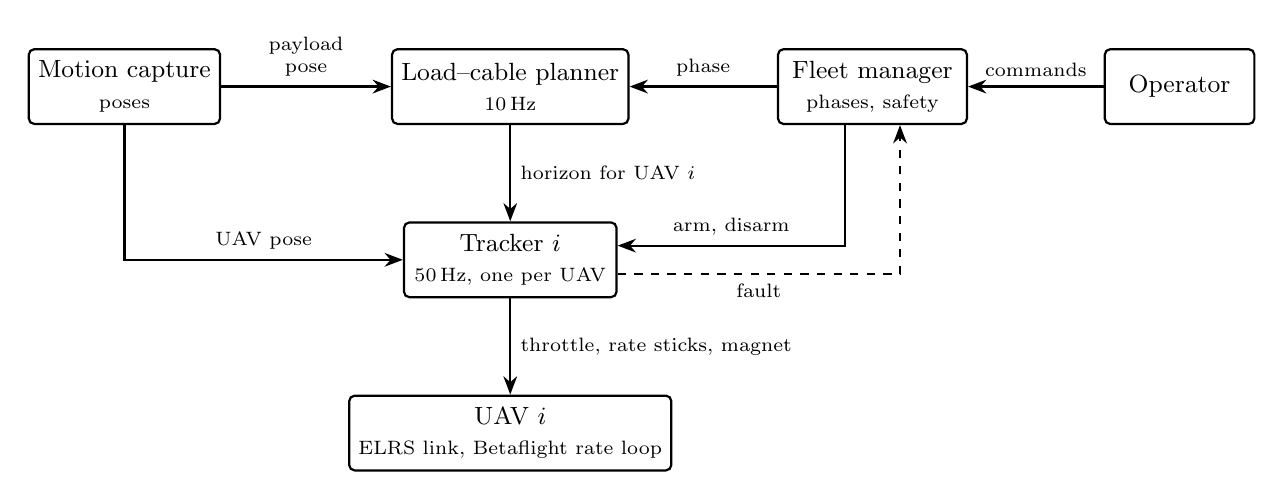
\begin{tikzpicture}[>=Stealth,
    blk/.style={draw, thick, rounded corners=2pt, align=center, minimum height=0.95cm, font=\small},
    lab/.style={font=\scriptsize, align=center}]
  \node[blk, minimum width=2.4cm] (mocap) at (0,0) {Motion capture\\ \scriptsize poses};
  \node[blk, minimum width=2.7cm] (plan) at (4.9,0) {Load--cable planner\\ \scriptsize 10\,Hz};
  \node[blk, minimum width=2.4cm] (fm) at (9.5,0) {Fleet manager\\ \scriptsize phases, safety};
  \node[blk, minimum width=1.9cm] (op) at (13.4,0) {Operator};
  \node[blk, minimum width=2.7cm] (trk) at (4.9,-2.2) {Tracker $i$\\ \scriptsize 50\,Hz, one per UAV};
  \node[blk, minimum width=2.7cm] (uav) at (4.9,-4.4) {UAV $i$\\ \scriptsize ELRS link, Betaflight rate loop};
  \draw[->, thick] (mocap) -- node[lab, above] {payload\\ pose} (plan);
  \draw[->, thick] (mocap.south) |- node[lab, pos=0.75, above] {UAV pose} (trk.west);
  \draw[->, thick] (plan) -- node[lab, right] {horizon for UAV $i$} (trk);
  \draw[->, thick] (trk) -- node[lab, right] {throttle, rate sticks, magnet} (uav);
  \draw[->, thick] (fm) -- node[lab, above] {phase} (plan);
  \draw[->, thick] (op) -- node[lab, above] {commands} (fm);
  \draw[->, thick] ([xshift=-0.35cm]fm.south) |- node[lab, pos=0.75, above] {arm, disarm} ([yshift=0.18cm]trk.east);
  \draw[->, thick, dashed] ([yshift=-0.18cm]trk.east) -| node[lab, pos=0.25, below] {fault} ([xshift=0.35cm]fm.south);
\end{tikzpicture}
\caption[Nodes and links]{Nodes and links. Solid: commands, references and poses; dashed: a tracker
reporting a fault, which disarms the whole fleet. The operator's commands are ARM, TAKEOFF, LAND,
DETACH and ATTACH.}
\label{fig:nodes}
\end{figure}

The system has three layers.
\begin{description}
    \item[Planner.] The centralised load--cable MPC of Section~\ref{sec:controller}. At 10\,Hz it
    plans the motion of the payload and of every rod, and publishes to each UAV its reference over
    the horizon: position, velocity, acceleration, the planned cable acceleration and the throttle
    feedforward. A second reference generator, the dissipative network of
    Section~\ref{sec:dissipative}, can replace it in flight; both publish the same reference format,
    so the trackers do not know which one is active.
    \item[Trackers.] One tracking MPC per UAV at 50\,Hz. Each follows its UAV's part of the plan and
    turns it into the radio commands.
    \item[Fleet manager.] It sequences the phases of a flight: ARM, TAKEOFF (the climb, the rod sweep
    to the working elevation and the lift), the trajectory, LAND, and the reconfiguration events
    DETACH and ATTACH (Section~\ref{sec:reconfig}).
\end{description}
\paragraph{Safety.} Every tracker checks its own UAV against a flight envelope: tilt, payload tilt
(both 60$^\circ$) and speed (3\,m/s). It also checks that its motion-capture pose is fresh (0.25\,s)
and that the planner's reference is fresh (1\,s). Any violation disarms the whole fleet, not the one
UAV: a single UAV losing thrust on a shared rigid payload drags the others with it. There is no
geofence; the operator holds a kill switch. On the rig, each UAV must also confirm that its flight
controller is armed before the fleet takes off. The planner stops iterating at a 60\,ms budget,
and a plan that has not converged by then is replaced by the previous one, shifted by a tick.
A UAV that disarms between ARM and TAKEOFF grounds the whole fleet and TAKEOFF is refused,
since three UAVs lifting a ring sized for four would drag it.

\subsubsection{Rig hardware}
\label{sec:hardware}

\paragraph{UAVs.} Four UAVs run Betaflight in rate mode on six-cell batteries. Each has its own
ELRS receiver and a ground transmitter on a USB serial port, so every UAV is commanded on its
own link at 100\,Hz. The throttle, three rate sticks, the arm switch and an auxiliary channel are
sent; the auxiliary channel switches the UAV's magnet and is held on from start-up, so a quiet link
cannot drop the payload. The flight controller's telemetry (battery voltage, flight mode, link
quality) comes back on the same link. As flown, each UAV weighs 0.55\,kg: an airframe and battery of
0.475\,kg, plus its rod and magnet.

\paragraph{Rods and payload.} Each UAV carries a rigid rod of 0.55\,m and 0.075\,kg with a ball joint
at both ends. The upper joint sits 4\,cm below the UAV's centre. The payload is a 0.86\,kg ring of
0.51\,m diameter and 40\,mm thickness, with twelve magnet plates every 30$^\circ$ on its top face at a
radius of 0.225\,m.
Each rod ends in an electromagnet that holds on a plate with 10--12\,N and releases under a jerk.
A layout is named by its plate numbers, anticlockwise from plate 0 on the ring's $+x$ axis
(Figure~\ref{fig:geometry}).

% fig_geometry.tex -- M3: payload and rod geometry (TikZ). Dimensions from the rig (30 Sep 2026):
% plates at r 0.225 m on a 500 mm ring, 12 plates every 30 deg anticlockwise from +x, rod 0.55 m,
% pivot 4 cm below the UAV centre, working elevation 45 deg. Drawn to scale (1 m = 9 cm).
\begin{figure}[h]
\centering
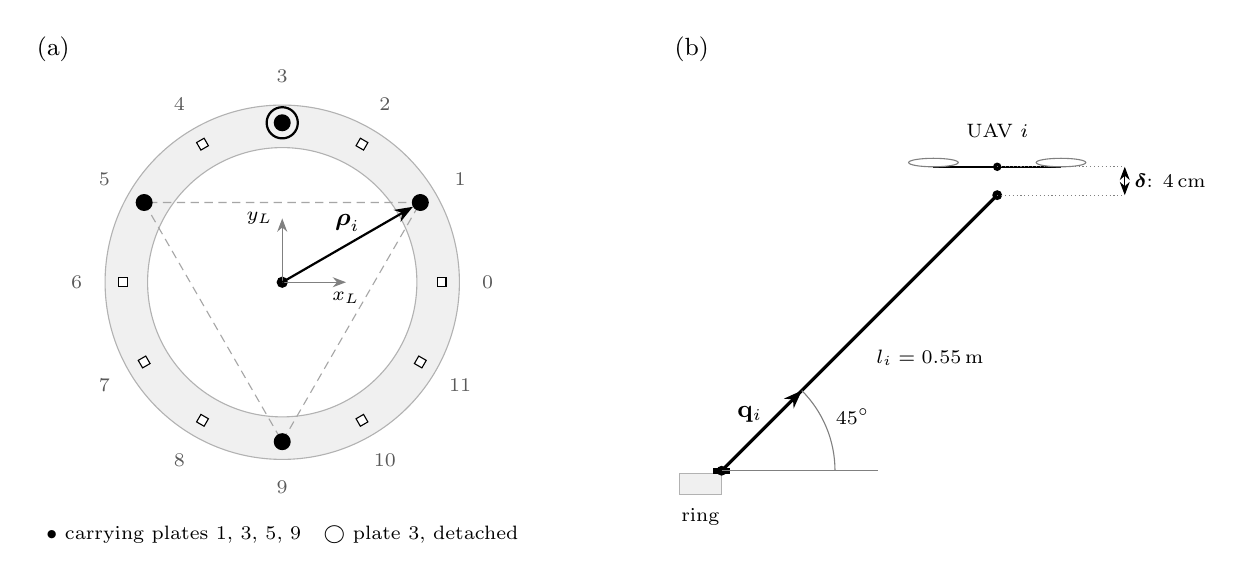
\begin{tikzpicture}[x=9cm, y=9cm, >=Stealth, font=\small]
  % ---------------- (a) top view ----------------
  \begin{scope}
    \fill[gray!12] (0,0) circle (0.25);
    \fill[white] (0,0) circle (0.19);
    \draw[gray!60, thin] (0,0) circle (0.25) (0,0) circle (0.19);
    % the even triangle left after detaching plate 3
    \draw[densely dashed, gray!70] (30:0.225) -- (150:0.225) -- (270:0.225) -- cycle;
    % plates
    \foreach \k in {0,...,11} {
      \pgfmathsetmacro{\a}{30*\k}
      \node[draw, fill=white, minimum size=0.11cm, inner sep=0pt, rotate=\a] at (\a:0.225) {};
      \node[font=\scriptsize, text=gray!70!black] at (\a:0.29) {\k};
    }
    % the four carrying plates
    \foreach \k in {1,3,5,9} { \fill[black] (30*\k:0.225) circle (0.012); }
    \draw[thick, black] (90:0.225) circle (0.022);
    % centre, axes, rho
    \fill (0,0) circle (0.008);
    \draw[->, thin, gray] (0,0) -- (0.09,0) node[below, font=\scriptsize, text=black] {$x_L$};
    \draw[->, thin, gray] (0,0) -- (0,0.09) node[left, font=\scriptsize, text=black] {$y_L$};
    \draw[->, thick] (0,0) -- (30:0.213) node[pos=0.62, above left, inner sep=1pt] {$\boldsymbol{\rho}_i$};
    \node[font=\scriptsize, align=left, anchor=north] at (0,-0.33) {$\bullet$ carrying plates 1, 3, 5, 9\quad $\bigcirc$ plate 3, detached};
    \node[anchor=north west] at (-0.36,0.36) {(a)};
  \end{scope}
  % ---------------- (b) side view of one rod (A plate, P pivot, C UAV centre) ----------------
  \begin{scope}[shift={(0.62,-0.30)}]
    \fill[gray!12] (-0.06,0) rectangle (0.0,0.03);
    \draw[gray!60, thin] (-0.06,0) rectangle (0.0,0.03);
    \fill[black] (-0.012,0.03) rectangle (0.012,0.038);
    \coordinate (A) at (0,0.034);
    \coordinate (P) at (0.3889,0.4229);
    \coordinate (C) at (0.3889,0.4629);
    \draw[very thick] (A) -- (P);
    \fill (A) circle (0.007) (P) circle (0.007);
    \draw[thick] (0.2989,0.4629) -- (0.4789,0.4629);
    \draw[gray] (0.2989,0.4689) ellipse (0.035 and 0.006) (0.4789,0.4689) ellipse (0.035 and 0.006);
    \fill (C) circle (0.006);
    \draw[->, thick] (A) -- (0.1131,0.1471) node[pos=0.55, above left, inner sep=1pt] {$\mathbf{q}_i$};
    \draw[gray] (0.16,0.034) arc (0:45:0.16);
    \draw[gray, thin] (A) -- (0.22,0.034);
    \node[font=\scriptsize] at (0.185,0.1105) {45$^\circ$};
    \node[font=\scriptsize, anchor=north west] at (0.2045,0.2185) {$l_i = 0.55$\,m};
    \draw[gray, thin, densely dotted] (P) -- (0.5689,0.4229) (C) -- (0.5689,0.4629);
    \draw[<->, thin] (0.5689,0.4229) -- (0.5689,0.4629) node[midway, right, font=\scriptsize] {$\boldsymbol{\delta}$: 4\,cm};
    \node[font=\scriptsize, anchor=north] at (-0.03,-0.005) {ring};
    \node[font=\scriptsize, anchor=south] at (0.3889,0.49) {UAV $i$};
    \node[anchor=north west] at (-0.08,0.66) {(b)};
  \end{scope}
\end{tikzpicture}
\caption[Payload and rod geometry]{Payload and rod geometry, to scale. (a) Top view of the 0.86\,kg ring
with its twelve magnet plates at a radius of 0.225\,m, numbered anticlockwise from the $x_L$ axis. The
four-UAV layout uses plates 1, 3, 5 and 9; detaching the UAV on plate 3 leaves the even triangle
(dashed), under which the ring hangs level. (b) Side view of one rod at the working elevation: the rod
direction $\mathbf{q}_i$ points from the plate to the UAV, and the rod pivots $\boldsymbol{\delta}$ = 4\,cm
below the UAV's centre.}
\label{fig:geometry}
\end{figure}


Figure~\ref{fig:rig_photo} shows the rig.

\pendingfig{fig:rig_photo}{The rig: four UAVs on rods, the ring with its twelve magnet plates, the motion-capture markers and the newcomer's magnet tip.}{photograph at the 14 Oct setup}

\paragraph{Motion capture.} OptiTrack tracks one rigid body per UAV and one for the ring. Its poses
are the only state measurement: the velocities and body rates of the UAVs and of the ring are
differentiated from them.


% model.tex -- Methodology: the system model, stated once in the planner's notation.
% Merged 9 Oct (structure audit) from the literature review's payload model (modelling.tex,
% "Cable-Suspended Payload Dynamics") and the planner's model (controller.tex, "Load--cable planner").
% Where the two notations conflicted the planner's is kept. What changed from the review's version:
%  - the rod force T_i is written lambda_i q_i, with q_i pointing from the attachment point to UAV i;
%  - the payload moment is lambda_i rho_i x R_L^T q_i in the payload frame (was rho_i x T_i, frame
%    unstated);
%  - the payload attitude is the quaternion q_L with rotation R_L (was R_L only), and its velocity v_L;
%  - the UAV's equation m_q pddot_i = R_i f_i e3 - m_q g e3 - T_i (scalar thrust f_i along body z) is
%    replaced by the thrust vector f_i each UAV must produce, eq:thrust_req, which is the same equation
%    solved for the thrust; the UAV attitude R_i is then the direction of f_i;
%  - the UAV positions are not states: they follow from the rod kinematics (eq:rod_kin), with the pivot
%    offset delta; the state count is 13 + 14N (the review counted UAV states instead);
%  - a constant force d on the payload is added for steady-error rejection.
% The code (mpc_planner, after Sun et al.) uses s_i = -q_i and t_i = lambda_i.

\subsection{Model and planner}
\label{sec:model}

\subsubsection{System model}

The controller's model follows the load--cable formulation of \cite{tudelft} with the standard
simplifications of Section~\ref{sec:lit_models}: the payload is a rigid body of known mass and inertia,
and each link a rigid, massless rod, taut at all times, whose direction and tension are states. The
formulation calls the links cables, hence the names load--cable planner and cable feedforward (the rod's
planned pull passed to the trackers). The fixed team of the literature
\cite{efficient, wahbaKinodynamicMotionPlanning2024, quan2025swarm} is relaxed so that UAVs can join or
leave mid-flight:
the attachment points and rod lengths are runtime parameters, and the team size selects a solver
(Section~\ref{sec:reconfig}).

The payload has mass $m_L$, inertia $\mathbf{J}_L \in \mathbb{R}^{3\times3}$, position $\mathbf{p}_L$,
velocity $\mathbf{v}_L$, attitude quaternion $\mathbf{q}_L$ (rotation $R_L$) and angular velocity
$\boldsymbol{\omega}_L$ in its own frame. $N$ UAVs pull on it through rods of length $l_i$ attached at
$\boldsymbol{\rho}_i$, offset from the payload's centre of mass (CoM) in the payload frame
(Figures~\ref{fig:geometry} and~\ref{fig:payload_system}). The rod direction $\mathbf{q}_i \in S^2$ points
from the attachment point to UAV $i$, and the rod pulls on the payload with
$\mathbf{T}_i = \lambda_i \mathbf{q}_i$, $\lambda_i \ge 0$.

\begin{figure}[h]
\centering
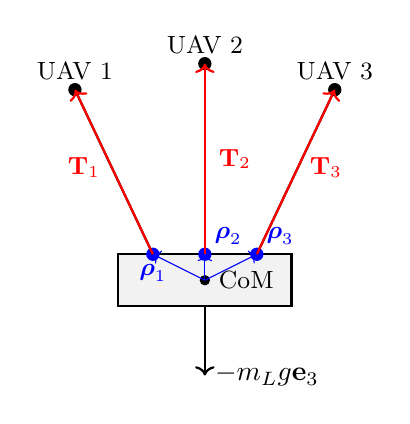
\begin{tikzpicture}[scale=1.1]
  % Payload box
  \draw[thick,fill=gray!10] (-1.0,-0.3) rectangle (1.0,0.3);

  % Centre of mass marker
  \filldraw (0,0) circle (1.5pt);
  \node[right, font=\small] at (0.05,0) {CoM};

  % Gravity
  \draw[->,thick] (0,-0.3) -- (0,-1.1) 
      node[right] {$-m_L g \mathbf{e}_3$};

  % Attachment points on payload surface
  \filldraw[blue] (-0.6,0.3) circle (2pt);
  \filldraw[blue] (0.0,0.3) circle (2pt);
  \filldraw[blue] (0.6,0.3) circle (2pt);

  % UAV 1 - left
  \filldraw (-1.5, 2.2) circle (2pt);
  \node[above, font=\small] at (-1.5,2.2) {UAV 1};
  \draw[thick] (-1.5,2.2) -- (-0.6,0.3);
  \draw[->,red,thick] (-0.6,0.3) -- (-1.5,2.2);
  \node[left, font=\small, red] at (-1.1,1.3) {$\mathbf{T}_1$};
  \draw[->,blue] (0,0) -- (-0.6,0.3) 
      node[below, font=\small, blue] {$\boldsymbol{\rho}_1$};

  % UAV 2 - centre
  \filldraw (0, 2.5) circle (2pt);
  \node[above, font=\small] at (0,2.5) {UAV 2};
  \draw[thick] (0,2.5) -- (0,0.3);
  \draw[->,red,thick] (0,0.3) -- (0,2.5);
  \node[right, font=\small, red] at (0.05,1.4) {$\mathbf{T}_2$};
  \draw[->,blue] (0,0) -- (0,0.3)
      node[above right, font=\small, blue] {$\boldsymbol{\rho}_2$};

  % UAV 3 - right
  \filldraw (1.5, 2.2) circle (2pt);
  \node[above, font=\small] at (1.5,2.2) {UAV 3};
  \draw[thick] (1.5,2.2) -- (0.6,0.3);
  \draw[->,red,thick] (0.6,0.3) -- (1.5,2.2);
  \node[right, font=\small, red] at (1.1,1.3) {$\mathbf{T}_3$};
  \draw[->,blue] (0,0) -- (0.6,0.3)
      node[above right, font=\small, blue] {$\boldsymbol{\rho}_3$};

\end{tikzpicture}
\caption[Multi-UAV payload system]{Multi-UAV payload system: rod $i$ pulls on the payload with tension $\mathbf{T}_i = \lambda_i \mathbf{q}_i$ at the attachment point $\boldsymbol{\rho}_i$, offset from the payload's CoM.}
\label{fig:payload_system}
\end{figure}

Rod $i$ contributes its direction $\mathbf{q}_i$, the angular velocity of that direction $\mathbf{r}_i$
and its first two derivatives, and the tension $\lambda_i$ with its rate:
\begin{equation}
    \mathbf{x} = \big[\, \mathbf{p}_L,\ \mathbf{v}_L,\ \mathbf{q}_L,\ \boldsymbol{\omega}_L,\
    \{\mathbf{q}_i,\ \mathbf{r}_i,\ \dot{\mathbf{r}}_i,\ \ddot{\mathbf{r}}_i,\ \lambda_i,\ \dot{\lambda}_i\}_{i=1}^{N} \,\big]
    \in \mathbb{R}^{13+14N}.
\end{equation}
The inputs are the third derivative of each rod's angular velocity and the second derivative of its
tension, $\mathbf{u} = \{\boldsymbol{\gamma}_i, \eta_i\}_{i=1}^N$, so that the tensions and the rod
directions, and with them the UAV accelerations, are smooth. The dynamics are the payload's
Newton--Euler equations and the rod kinematics:
\begin{align}
    \dot{\mathbf{p}}_L &= \mathbf{v}_L, &
    m_L \dot{\mathbf{v}}_L &= \sum_{i=1}^{N} \lambda_i \mathbf{q}_i - m_L g \mathbf{e}_3 + \mathbf{d},
    \label{eq:plan_trans} \\
    \dot{\mathbf{q}}_L &= \tfrac{1}{2}\, \mathbf{q}_L \otimes \begin{bmatrix} 0 \\ \boldsymbol{\omega}_L \end{bmatrix}, &
    \mathbf{J}_L \dot{\boldsymbol{\omega}}_L &= \sum_{i=1}^{N} \lambda_i\, \boldsymbol{\rho}_i \times R_L^\top \mathbf{q}_i
    - \boldsymbol{\omega}_L \times \mathbf{J}_L \boldsymbol{\omega}_L, \\
    \dot{\mathbf{q}}_i &= \mathbf{r}_i \times \mathbf{q}_i, &
    \dddot{\mathbf{r}}_i &= \boldsymbol{\gamma}_i, \qquad \ddot{\lambda}_i = \eta_i,
\end{align}
where $\mathbf{d}$ is a constant force on the payload, zero in the original formulation and used for
steady-error rejection in Section~\ref{sec:disturbance}. The UAV positions follow from the rod
kinematics,
\begin{equation}
    \mathbf{p}_i = \mathbf{p}_L + R_L \boldsymbol{\rho}_i + l_i \mathbf{q}_i - \boldsymbol{\delta},
    \label{eq:rod_kin}
\end{equation}
with $\boldsymbol{\delta}$ the position of the rod pivot relative to the UAV's
centre ($\boldsymbol{\delta} = -0.04\,\mathbf{e}_3$\,m on the rig). The rod tension couples the system:
it drives the payload in \eqref{eq:plan_trans} and acts, equal and opposite, on UAV $i$.
Differentiating \eqref{eq:rod_kin} twice gives $\ddot{\mathbf{p}}_i$, and the thrust each UAV of mass
$m_q$ must produce is
\begin{equation}
    \mathbf{f}_i = m_q\big(\ddot{\mathbf{p}}_i + g\mathbf{e}_3\big) + \lambda_i \mathbf{q}_i .
    \label{eq:thrust_req}
\end{equation}
The state grows linearly with $N$, which drives the computational scaling noted in \cite{tudelft}.


% controller.tex -- draft of the controller as flown (4 Oct 2026), input from Methodology.tex.
% Notation follows Source/src/model.tex: q_i points from the payload attachment to UAV i and
% T_i = lambda_i q_i. The code (mpc_planner, after Sun et al.) uses s_i = -q_i and t_i = lambda_i.
% Restructured 9 Oct (structure audit): the model moved to model.tex; planner, tracker and steady-error
% rejection are subsections of their own; the result numbers (the box's effect, K's measured values,
% the damping ratio) moved to Section 4.2; the thrust identification procedure moved here from
% hardware.tex; the cost weights moved to Appendix B. Notation: the horizon has N_h nodes over T_h
% (were N and T, which also named the team size and the tension).
% Its references (francis1976internal, pannocchia2003disturbance, pannocchia2007combined,
% maeder2009linear, verschueren2022acados) are in references.bib.

\subsection{Load--cable planner}
\label{sec:controller}

The controller is a two-level cascade of model predictive controllers (Figure~\ref{fig:cascade}).
A centralised planner, based on the load--cable formulation of \cite{tudelft}, plans the motion of
the payload and of every rod over a horizon. Each UAV runs its own tracking MPC, which follows the
planner's reference for that UAV and accounts for the planned rod force. The tracker's output
(collective throttle and three body-rate commands) is sent over the radio link to the flight
controller, whose inner rate loop is not modified. Both levels are solved with acados
\cite{verschueren2022acados} using a real-time iteration (RTI) scheme \cite{diehl2002rti}: one
Gauss--Newton SQP step per tick, warm-started from the previous solution, with the QPs solved by
HPIPM \cite{frison2020hpipm} (partial condensing in the planner, full condensing in the tracker).
Both horizons have $N_h = 20$ nodes over $T_h = 2$\,s.

\begin{figure}[h]
\centering
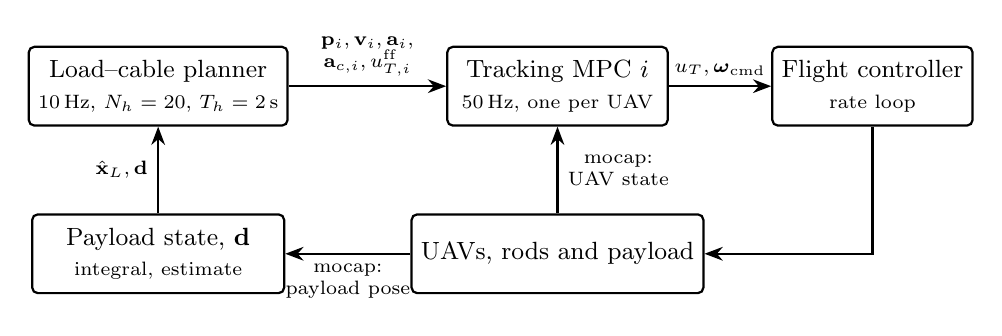
\begin{tikzpicture}[node distance=1.0cm and 1.3cm, >=Stealth,
    blk/.style={draw, thick, rounded corners=2pt, align=center, minimum height=1.0cm, font=\small},
    lab/.style={font=\scriptsize, align=center}]
  \node[blk, minimum width=3.2cm] (plan) {Load--cable planner\\ \scriptsize 10\,Hz, $N_h=20$, $T_h=2$\,s};
  \node[blk, right=2.0cm of plan, minimum width=2.8cm] (trk) {Tracking MPC $i$\\ \scriptsize 50\,Hz, one per UAV};
  \node[blk, right=1.3cm of trk, minimum width=2.2cm] (fc) {Flight controller\\ \scriptsize rate loop};
  \node[blk, below=1.1cm of trk, minimum width=2.8cm] (sys) {UAVs, rods and payload};
  \node[blk, below=1.1cm of plan, minimum width=3.2cm] (dist) {Payload state, $\mathbf{d}$\\ \scriptsize integral, estimate};
  \draw[->, thick] (plan) -- node[lab, above] {$\mathbf{p}_i, \mathbf{v}_i, \mathbf{a}_i,$\\ $\mathbf{a}_{c,i}, u_{T,i}^{\mathrm{ff}}$} (trk);
  \draw[->, thick] (trk) -- node[lab, above] {$u_T, \boldsymbol{\omega}_{\mathrm{cmd}}$} (fc);
  \draw[->, thick] (fc) |- (sys);
  \draw[->, thick] (sys) -- node[lab, right] {mocap:\\ UAV state} (trk);
  \draw[->, thick] (sys) -- node[lab, below] {mocap:\\ payload pose} (dist);
  \draw[->, thick] (dist) -- node[lab, left] {$\hat{\mathbf{x}}_L, \mathbf{d}$} (plan);
\end{tikzpicture}
\caption[Controller structure]{Controller structure. Motion capture closes both loops; the disturbance term enters the
planner's model.}
\label{fig:cascade}
\end{figure}

The planner works on the model of Section~\ref{sec:model}.

\paragraph{Optimal control problem.} At each planner tick the planner solves
\begin{equation}
\begin{aligned}
    \min_{\mathbf{x}_{0:N_h},\, \mathbf{u}_{0:N_h-1}} \quad & \sum_{k=0}^{N_h-1} \big\| \mathbf{y}(\mathbf{x}_k, \mathbf{u}_k) - \mathbf{y}_k^{\mathrm{ref}} \big\|_{W}^{2}
    + \big\| \mathbf{y}_{N_h}(\mathbf{x}_{N_h}) - \mathbf{y}_{N_h}^{\mathrm{ref}} \big\|_{W_{N_h}}^{2} \\
    \text{s.t.} \quad & \mathbf{x}_{k+1} = \mathbf{F}(\mathbf{x}_k, \mathbf{u}_k; \mathbf{d}), \\
    & C_0 \mathbf{x}_0 = C_0 \hat{\mathbf{x}}(t), \\
    & \lambda_{\min} \le \lambda_{i,k} \le \lambda_{\max}, \quad f_{\min} \le \|\mathbf{f}_{i,k}\| \le f_{\max}, \\
    & |\boldsymbol{\gamma}_{i,k}| \le \gamma_{\max}, \quad |\eta_{i,k}| \le \eta_{\max},
\end{aligned}
\label{eq:plan_ocp}
\end{equation}
with the output
$\mathbf{y} = [\mathbf{p}_L, \mathbf{v}_L, \mathbf{e}_R, \boldsymbol{\omega}_L, \{\mathbf{q}_i\}, \{\lambda_i\}, \{\mathbf{r}_i\}, \mathbf{u}]$,
where $\mathbf{e}_R = 2\,\mathrm{vec}(\mathbf{q}_L^{\mathrm{ref}} \otimes \mathbf{q}_L^{*})$ is the sign-invariant
attitude error. The thrust bounds are softened with slack. $\mathbf{F}$ is the integrated dynamics
over one node of $T_h/N_h = 0.1$\,s.

The initial-condition constraint pins only what motion capture measures directly: the payload pose
and twist, and each rod direction ($C_0$ selects $\mathbf{p}_L, \mathbf{v}_L, \mathbf{q}_L,
\boldsymbol{\omega}_L, \mathbf{q}_i$). The rod rates and their derivatives and the tensions are free
decision variables at node 0, warm-started from the previous solution. Pinning a tension carried over
from the last plan against a measured pose that the UAVs did not quite reach makes node 0 inconsistent.

\paragraph{References.} The payload reference $(\mathbf{p}_L^{\mathrm{ref}}, \mathbf{v}_L^{\mathrm{ref}},
\mathbf{a}_L^{\mathrm{ref}})$ comes from the lift schedule and the trajectory. The rod references are
derived from it by flatness. Holding the payload against gravity, its acceleration and the force
$\mathbf{d}$ needs the rods to support the effective gravity
\begin{equation}
    \mathbf{g}_{\mathrm{eff}} = g\mathbf{e}_3 + \mathbf{a}_{L,xy}^{\mathrm{ref}} - \mathbf{d}/m_L ,
\end{equation}
where $\mathbf{a}_{L,xy}^{\mathrm{ref}}$ is the horizontal part of the reference acceleration (the
trajectories are level),
and the nominal formation (each rod at 45$^\circ$ elevation, tensions $\lambda_i^{0}$ balancing the payload
weight) is rotated so that its vertical axis lies along $\mathbf{g}_{\mathrm{eff}}$, and the tensions are
scaled to $\lambda_i^{\mathrm{ref}} = \lambda_i^{0}\, \|\mathbf{g}_{\mathrm{eff}}\| / g$.

The weights are listed in Table~\ref{tab:weights} (Appendix~\ref{sec:app_params}). The weight on the rod
directions holds the formation's shape, and the weight on the rod rates damps rod swing.

\paragraph{Output to the trackers.} From the solved horizon the planner sends each tracker its
reference position, velocity and acceleration from \eqref{eq:rod_kin}, the planned cable acceleration
$\mathbf{a}_{c,i} = -\lambda_i \mathbf{q}_i / m_q$ at every node, and a throttle feedforward from
$\|\mathbf{f}_i\|$ in \eqref{eq:thrust_req}. The reference is the whole horizon, not a single
set-point, and the tracker interpolates it at its own rate, so a late or skipped planner tick does not
leave it without a reference.

\subsection{UAV tracking MPC and thrust map}
\label{sec:tracker}

Each UAV $i$ runs a tracking MPC on a 17-state model, in which the four stick channels sent to the
flight controller are themselves states and their rates of change are the inputs:
\begin{equation}
    \mathbf{x}_i = [\mathbf{p},\ \mathbf{q},\ \mathbf{v},\ \boldsymbol{\omega},\ \mathbf{c}], \qquad
    \mathbf{c} = [c_\phi, c_\theta, u_T, c_\psi], \qquad \mathbf{u}_i = \dot{\mathbf{c}},
\end{equation}
with
\begin{align}
    \dot{\mathbf{p}} &= \mathbf{v}, &
    \dot{\mathbf{q}} &= \tfrac{1}{2}\, \Omega(\boldsymbol{\omega})\, \mathbf{q}, \\
    \dot{\mathbf{v}} &= R(\mathbf{q})\, k_T u_T \mathbf{e}_3 - g\mathbf{e}_3 - c_z v_z \mathbf{e}_3 + \mathbf{a}_{c,i}, &
    \dot{\boldsymbol{\omega}} &= \frac{1}{\tau_\omega}\big(\boldsymbol{\omega}_{\mathrm{cmd}}(\mathbf{c}) - \boldsymbol{\omega}\big),
    \label{eq:trk_model}
\end{align}
where $\boldsymbol{\omega}_{\mathrm{cmd}}(\mathbf{c})$ is the flight controller's rate curve applied to the
roll, pitch and yaw sticks, and $\tau_\omega$ the time constant of its rate loop. Thrust is modelled
as affine in throttle, identified on the rig: the throttle sent is $u_T + u_0(V)$, with the offset
$u_0(V) = u_0 + \kappa (V_{\mathrm{ref}} - V)$ correcting for the battery voltage $V$ and $k_T$ the gain
above it. The planned cable acceleration $\mathbf{a}_{c,i}$ enters the model as a known, time-varying
parameter along the horizon, so the tracker anticipates the rod's pull instead of reacting to it.
The planned pull is only as good as the planner's model of the rods. On the rig the rods flew at about
60$^\circ$ from horizontal where the plan assumed 45$^\circ$, so each tracker now measures the pull and uses the
plan only for its shape along the horizon: the measured pull is the UAV's acceleration from motion capture
(the least-squares slope of its velocity over 80\,ms, low-pass filtered at 50\,ms) minus the modelled thrust,
gravity and drag, with the thrust passed through the same filter so that a throttle change does not read as
a change of pull. The horizon's planned pull is shifted by the difference between the measured and the
planned pull at its first node, and the result is capped at 12\,m/s$^2$. The planner plans the rods at
60$^\circ$ to match. Section~\ref{sec:res_rig_integral} gives its effect on the rig.

The tracker solves, every 20\,ms,
\begin{equation}
\begin{aligned}
    \min \quad & \sum_{k=0}^{N_h-1} \big\| \mathbf{h}(\mathbf{x}_k, \mathbf{u}_k) - \mathbf{h}_k^{\mathrm{ref}} \big\|_{Q}^{2} + \big\| \mathbf{h}_{N_h}(\mathbf{x}_{N_h}) - \mathbf{h}_{N_h}^{\mathrm{ref}} \big\|_{Q_{N_h}}^{2} \\
    \text{s.t.} \quad & \mathbf{x}_{k+1} = \mathbf{F}_i(\mathbf{x}_k, \mathbf{u}_k; \mathbf{a}_{c,i,k}), \qquad \mathbf{x}_0 = \hat{\mathbf{x}}_i(t), \\
    & 0.05 \le u_{T,k} \le u_{T,\max}, \quad |c_{\phi,k}|, |c_{\theta,k}|, |c_{\psi,k}| \le 1, \quad |\mathbf{u}_k| \le \overline{\mathbf{u}},
\end{aligned}
\label{eq:trk_ocp}
\end{equation}
with $\mathbf{h} = [\mathbf{p}, \mathbf{v}, \boldsymbol{\omega}, \mathbf{c}, \mathbf{u}, \mathbf{e}_R]$, the
attitude reference being the direction of the planned thrust \eqref{eq:thrust_req}. The stick states
are normalised to $[-1, 1]$, and $\overline{\mathbf{u}}$ limits how fast each may change (throttle
0.5\,s$^{-1}$). Only the first command of each solution is sent.

\paragraph{Initial condition.} Node 0 equals the measured state, $\mathbf{x}_0 = \hat{\mathbf{x}}_i(t)$,
which is the standard formulation. The stick states in $\hat{\mathbf{x}}_i$ are the commands actually
sent, not the last solution, so the model starts from where the actuators are. An earlier version
relaxed this to the box $\hat{\mathbf{x}}_i(1-\epsilon) \le \mathbf{x}_0 \le \hat{\mathbf{x}}_i(1+\epsilon)$
with $\epsilon = 0.025$; Section~\ref{sec:res_ic} shows its effect.

\paragraph{Thrust identification.} A proportional map with one gain, identified at hover, did not
hold across loads and battery states. The map was therefore identified on the rig: each UAV hovered
free with hung masses of 0, 98 and 196\,g over battery voltages of 22.7--24.6\,V, and the throttle it
needed was fitted against the mass it carried and the voltage. The fit and $k_T$ are in
Section~\ref{sec:thrust_id}.

\subsection{Steady-error rejection}
\label{sec:disturbance}

Any error that remains constant, from a model mismatch or an external force, is represented by the
constant force $\mathbf{d}$ on the payload in \eqref{eq:plan_trans}. $\mathbf{d}$ is a lumped disturbance:
for an external force (wind, a push, an unmodelled object in the basket) it is that force; for an
internal error (a thrust-map error, the rods' mass) it is the force that would have the same effect on
the payload, which need not exist physically. In the offset-free MPC literature this is an input
disturbance model \cite{pannocchia2003disturbance, maeder2009linear}.

\paragraph{Integral action through the model.} $\mathbf{d}$ is formed from the integral of the payload's
position error $\mathbf{e}_k = \mathbf{p}_L^{\mathrm{ref}} - \mathbf{p}_L$, updated at each planner tick
$k$ (period $T_s = 0.1$\,s):
\begin{equation}
    \mathbf{b}_{k+1} = \mathrm{sat}_{\bar{b}}\!\big(\mathbf{b}_k + k_i T_s\, G_k\, \mathbf{e}_k\big), \qquad
    \mathbf{d}_k = -K \mathbf{b}_k, \qquad K = \mathrm{diag}(K_{xy}, K_{xy}, K_z).
    \label{eq:lumped_int}
\end{equation}
Here $\mathrm{sat}_{\bar{b}}$ bounds each component to $\pm\bar{b}$, and $G_k = \mathrm{diag}(g_{xy}, g_{xy}, g_z)
\in \{0,1\}^3$ is a gate. The gate integrates only in steady, taut flight: lift complete, not
descending or landing, every rod taut, a fresh pose, the payload slow ($<0.05$\,m/s) and the miss
under 0.25\,m. The vertical component also integrates through a slow level orbit. The horizontal
components require a stationary reference, so a value learned in hover is held through a trajectory. A low payload ($e_z > 0$) makes $d_z$ negative: the planner then believes the payload is
heavier and plans more rod tension. Once the payload rests on the floor at landing, $\mathbf{d}$ is
set to zero.

$K$ converts the integral from metres to newtons. It is set to the closed-loop stiffness of the
cascade to a force on the payload, measured by applying a known force and recording the steady
displacement (Section~\ref{sec:res_force}). With this choice the integral's loop gain is
$k_i$, the same as for the equivalent reference-shift form below.

\paragraph{Where $\mathbf{d}$ enters.} $\mathbf{d}_k$ is a parameter of the planner's problem, constant
over the horizon and refreshed at every tick. It enters the payload's translational dynamics
\eqref{eq:plan_trans}, so the plan predicts the payload's motion with the force included and chooses
tensions and UAV positions that counter it. It also enters the reference formation through the
effective gravity $\mathbf{g}_{\mathrm{eff}}$ of the references above, so the formation the cost draws
the solution towards is already tilted and tensioned to balance $\mathbf{d}$, and the cost does not
oppose the force balance.

\paragraph{Zero steady-state error.} Suppose the closed loop converges to an equilibrium at which the
gate is open ($G = I$) and no component of $\mathbf{b}$ is saturated. Then $\mathbf{b}_{k+1} = \mathbf{b}_k$
in \eqref{eq:lumped_int} gives $k_i T_s \mathbf{e} = \mathbf{0}$, so $\mathbf{e} = \mathbf{0}$, whatever
the constant cause. This is the internal model principle \cite{francis1976internal}: a constant
disturbance is rejected because the controller contains a model of a constant, the integrator. The
statement assumes stability; it does not give it. Approximating the cascade's response to $\mathbf{d}$
by a first-order lag with time constant $\tau$, each axis becomes
\begin{equation}
    \tau s^2 + s + k_i = 0, \qquad \zeta = \frac{1}{2\sqrt{k_i \tau}},
\end{equation}
so a faster integral costs damping (Section~\ref{sec:res_force} gives $\zeta$ for the measured $\tau$). Time delays through the planner and the radio link reduce the margin further.

\paragraph{What the integral learns.} Let an unmodelled constant force $\mathbf{F}$ act on the payload,
let $K_c$ be the cascade's actual stiffness to a force on the payload, and treat the cascade as
quasi-static (fast compared with the integral). The plan cancels the force it believes in, $\mathbf{d}$,
so the payload settles displaced by $K_c^{-1}(\mathbf{F} - \mathbf{d})$ and
$\mathbf{e} = -K_c^{-1}(\mathbf{F} - \mathbf{d}) = -K_c^{-1}(\mathbf{F} + K\mathbf{b})$. In continuous time
\eqref{eq:lumped_int} becomes
\begin{equation}
    \dot{\mathbf{b}} = k_i\,\mathbf{e} = -k_i K_c^{-1}\big(K\mathbf{b} + \mathbf{F}\big)
    \quad\Rightarrow\quad \mathbf{b} \to -K^{-1}\mathbf{F}, \qquad \mathbf{d} \to \mathbf{F},
\end{equation}
a first-order convergence at the rate $k_i K K_c^{-1}$ on each axis, with time constant $1/k_i = 2.5$\,s when
$K = K_c$. The believed force converges to the applied one whatever $K$ is: $K$ sets only the speed,
and too large a $K$ costs damping as too large a $k_i$ does. When the force is removed, $\mathbf{b}$
still holds $-K^{-1}\mathbf{F}$, so the payload overshoots by $K_c^{-1}\mathbf{F}$, the displacement the
force caused at onset, and the overshoot decays at the same rate. Section~\ref{sec:res_force} measures both: the
learned force against the applied one, and the overshoot on release.

\paragraph{Reference-shift form.} An earlier version added the height integral to the payload's height
target instead, $z_L^{\mathrm{ref}} \leftarrow z_L^{\mathrm{ref}} + b_z$. Both forms are integral action and
reach the same steady state. In the offset-free MPC literature they correspond to output and input
disturbance models, which differ in transient behaviour, not in the steady state
\cite{pannocchia2007combined}. The model form keeps the target fixed. Its plan predicts a payload
held at the target, which is what happens. The reference-shift form plans a move towards the shifted
target that never comes. The model form also extends to the horizontal axes.

The model form is the default, on the rig as well as in simulation. Where it is not used, the
reference-shift form flies instead, on the height only: wherever the fleet can attach or detach
mid-flight, since the problem is resized with the integral in it, and wherever the integral is
switched off. The rig flights so far used the reference-shift form, as a bounded safety net with
$k_i = 0.4$\,s$^{-1}$.
% STATUS 5 Oct 2026: int_mode auto (model where allowed, else reference): reference with kt_trim on,
% a resizing fleet, z_ki 0, offset_free on or dist_est ring/full (bringup real_mode.planner_options).

\paragraph{Bound.} $\bar{b} = 0.3$\,m bounds the force the integral can supply to $K\bar{b}$ (2.1\,N
vertically), enough for an unmodelled 0.1\,kg object. The bound is a safety measure: a larger error is
a fault, not a disturbance. A warning is raised at 70\,\% of it, so that a fault is reported rather than
silently covered.

\paragraph{Limits.} The integral corrects forces on the payload, not moments: a constant moment, such as
one UAV's thrust-map error, still tilts the payload. A miss larger than the gate is never integrated,
so an error that large stays (Section~\ref{sec:sim_robustness}). The integral is also slow
($1/k_i = 2.5$\,s): it removes constant and slowly varying forces, not impacts or gusts, which only a
force measured on board each UAV could counter quickly.

\paragraph{Alternatives.} Five other ways to remove a steady error were built and flown on the same
cases as the integral (Section~\ref{sec:sim_methods}):
\begin{description}
    \item[Force balance] estimates a constant force on the ring and one shared by the UAVs from the
    measured motion and the delivered thrust, and gives them to the planner's model
    \cite{muske2002disturbance}.
    \item[Offset-free observer] estimates the force from the planner's own prediction error, as in
    offset-free MPC \cite{pannocchia2003disturbance}.
    \item[Measured cable force] each tracker takes its rod's force from its measured acceleration and
    delivered thrust, the ground-side counterpart of the compensation from inertial measurements of
    \cite{tudelft}.
    \item[Thrust-gain trim] a per-UAV estimate of the throttle-to-acceleration gain, from the UAV's own
    measured acceleration and its static share of the rod force.
    \item[Rod mass in the planner] the rods' mass added to the planner's model.
\end{description}

% Under evaluation (sim only): option A, a direct estimate of d from the measured motion and the
% delivered thrust. Per sample, least squares over the tensions, d_L and a force d_D shared by the
% UAVs, from
%   UAV i:    m_q a_i = f_i R_i e3 - m_q g e3 - lambda_i q_i + d_D
%   payload:  m_L a_L = sum_i lambda_i q_i - m_L g e3 + d_L
% filtered by two first-order stages. In the code it is not yet combined with eq:lumped_int.



% takeoff_landing.tex -- Methodology: takeoff from the floor, lift and landing (draft 4 Oct 2026).
% Code: mpc_planner/creep_controller.py (arc creep, hand-over latch), planner_node.py (pretension,
% breakaway, ff_cap_release_s, lift ramp, LAND, TouchdownDetector), bringup/config/*.yaml.
% Evidence: 23 Sep rig non-lift (start_taut), 30 Sep rig review, R0817/R0818, R0834-R0839 (B2),
% R0807-R0816 (hand-over angle in the twin), RIG-1001-* (hand-over and rods on the rig).
% Condensed 12 Oct 2026 to the plan's half page; the detail is Appendix C "Floor start and landing in detail".
% Restructured 9 Oct (structure audit): the outcomes (the hand-over angle flown, fig:flight) moved to
% Section 4.1.

\subsubsection{Takeoff, lift and landing}
\label{sec:takeoff}

The planner assumes taut rods, but every flight starts and ends with the ring on the floor and the rods slack or
flat, where the UAVs sit about 0.7\,m from the ring's centre, outside the cone the planner's references put them
on; started from rest, the planner pulled the UAVs inwards over the ring instead of lifting it, the cause of the
first failed lifts on the rig. Four steps take a flight from the floor into the regime the planner models, and three
measures take it back; Appendix~\ref{sec:app_floor} gives each with its numbers and the failure it answers.
\begin{itemize}
    \item \textbf{Rod sweep.} On TAKEOFF each UAV is anchored where it rests and its rod is swept about its own
    attachment point from its measured elevation to the planned one (60$^\circ$ since 7 October), the UAV's
    reference riding the far end of the rod, so that the rod stays straight and the UAV never crosses over the
    ring. The planner takes over once every rod has held within 8$^\circ$ of the planned elevation for 1\,s, and
    measures each rod's length from motion capture at that hand-over for its model and its tautness gate.
    \item \textbf{Pretension and breakaway.} Every UAV's share of the planned pull then rises together from zero
    over 3\,s with the ring's height target at its resting height; a step here launched the ring and released two
    magnets on the rig. When the ring rises 1\,cm or faster than 0.03\,m/s it has broken free, and the fraction of
    the planned pull reached at that moment is frozen as a cap on the trackers' feedforward, released back to the
    full pull over 2\,s once the lift starts.
    \item \textbf{Lift.} The height target ramps to the target height at 0.1\,m/s, eased in and out, and the
    trajectory starts when the ramp completes.
    \item \textbf{Landing.} On LAND the ring's height target descends at 0.2\,m/s with the formation unchanged
    until the ring rests. A rigid rod then pushes a UAV descending straight down outward as the rod lengthens
    horizontally, which tipped UAVs over in the twin, so each UAV's reference unwinds along its rod's circle about
    the grounded attachment point before it descends (twin only: the rig's tethers go slack and it lands straight
    down); the planner blends each UAV's thrust and rod feedforward to plain hover over 1\,s instead of dropping
    the rod term at touchdown; and a UAV back at its resting height with the ring down idles armed until the fleet
    disarms, so that a UAV that lands first does not track a reference below the floor. Touchdown is declared when
    the UAVs stop following the descending reference for 1\,s after at least 5\,cm of descent, and the fleet
    manager disarms the fleet.
\end{itemize}


% reconfiguration.tex -- Methodology: reconfiguration (detach and attach). Draft 4 Oct 2026.
% Code: dissipative_planner/dissipative_node.py (_detach_ocp, _attach_ocp, _capture_weld_rho,
% partner hand-off), dissipative_planner/approach.py, drone_magnet (magnet_attachment_manager,
% elrs_mux, handover_policy, attach_target_publisher), bringup/bringup/graph_attach.py.
% Evidence: CURRENT_STATE 4.1, 4.2, 4.11; notes 2026-09-24_detach_land_fix, 2026-09-25_attach_ocp,
% 2026-09-27_m1_rejoin, 2026-09-27_m1_full, 2026-09-27_m2_handover.

\subsection{Reconfiguration by OCP resize}
\label{sec:reconfig}

A reconfiguration changes the number of UAVs carrying the payload in the air. In the final design both
directions are handled the same way: the planner switches to a solver for the new team size and carries
on. This subsection describes the detach, the attach, and the design each replaced.

\subsubsection{Detach}

On DETACH the departing UAV's magnet releases the rod at the payload end, the UAV flies away with its
rod, and the planner continues with the survivors. Two approaches were built and compared.

\paragraph{OCP resize.} The planner keeps flying the payload and re-solves for the smaller fleet, which
two properties of the formulation make possible.
\begin{itemize}
    \item The attachment points $\boldsymbol{\rho}_i$ and rod lengths $l_i$ are runtime parameters of
    the model, not constants compiled into the solver. Only the fleet size fixes the problem
    dimensions, so one solver per fleet size, built in advance, covers any attachment layout.
    \item The survivors keep their own attachment points. The rods stay where they were on the ring,
    so three survivors of a four-UAV ring sit, for example, at 0, 90 and 180$^\circ$, not at an even
    0, 120 and 240$^\circ$. Handing the planner an even ring instead makes its moment balance wrong by
    construction.
    \redo{the hand-back to an even ring after a detach from four UAVs (the survivors at 0, 90 and 180$^\circ$, the planner told 0, 120 and 240$^\circ$): payload tilt.}
% --- original text, flown before the rig twin; kept to refill this place:
%     0, 120 and 240$^\circ$. Handing the planner an even ring instead makes its moment balance wrong by
%     construction; in an early test this tipped the payload by 62$^\circ$.
\end{itemize}
At the detach the planner swaps to the solver for $N-1$ UAVs, sets the survivors' attachment points and
rod lengths, and warm-starts the new problem from the measured state. The tensions and rod directions are
free at node~0, so the first solve redistributes the load, with no separate hand-off phase. A detach is
refused if it would leave fewer than three UAVs, and during LAND.

\paragraph{Network hand-off.} The alternative, closer to the decentralised literature
\cite{quan2025swarm}, hands the payload to the dissipative network of Section~\ref{sec:dissipative} on the
detach; the network holds it while it redistributes the load between the survivors, then hands back to a
planner built for $N-1$. Section~\ref{sec:sim_detach} compares the two; the OCP resize is the detach used
in the rest of this work.
% --- original text, flown before the rig twin; kept to refill this place:
% then hands back to a planner built for $N-1$. In simulation the OCP resize won this comparison
% clearly (Section~\ref{sec:sim_detach}), and it is the detach used in the rest of this work.

% Departed landing (pressed to its rest, disarmed alone): twin 9 Oct, card 2026-10-09_departed_disarm_alone;
% the default once the LAND re-fly's reviewer passes it; rig W4/W5 on 14 Oct.
\paragraph{The departing UAV.} After the release, switched on the rig by the same DETACH command on the
UAV's magnet channel, the departing UAV steps 0.5\,m out radially at its height, clear of the ring and the
survivors, and lands on its own while the survivors carry on. Its height reference is pressed below its
own resting height until it gets there, and it is then disarmed alone, without waiting for the fleet
(Section~\ref{sec:res_detach_rig}).

\paragraph{Layout.} Whether the payload can still hang level after a detach depends on the geometry, not
on the controller: its centre of mass must stay inside the polygon of the surviving attachment points.
Removing one UAV from an even ring of $N$ leaves a largest angular gap of $4\pi/N$, which keeps the centre
inside only for $N \ge 5$; $N = 4$ sits exactly on the boundary. The four-UAV flights therefore use the
plates at 30, 90, 150 and 270$^\circ$, and detaching the UAV at 90$^\circ$ leaves an even triangle under
which the ring hangs level. With an uneven layout the planner's nominal tensions come from a moment
balance at the actual attachment points, so they are unequal and the payload's reference stays level.

\paragraph{Landing after a detach.} Touchdown is judged on the survivors only, so a departed UAV still
descending elsewhere does not hold their references down; a departed UAV is judged down at its own
resting height, and the fleet is declared landed only when it is down too. The cable feedforward is
switched off once the payload rests, because its sideways component pushes a grounded survivor across
the floor.
% --- original text, flown before the rig twin; kept to refill this place:
% declared landed only when they are down too. The cable feedforward is switched off once the payload
% rests, because its sideways component pushed a grounded survivor across the floor until it tipped
% in an early version.

\subsubsection{Attach}

On ATTACH a free UAV (the newcomer) approaches its attachment point, its magnet welds to a plate on the
ring, and the planner folds it into the team. The approach controller, the approach UAV and its magnet
are the collaborating student's; this work takes over at the weld.
% TODO: cite the collaborator's thesis or report once available.

\paragraph{Sequence.}
\begin{enumerate}
    \item \textbf{Target hold.} ATTACH freezes the payload's horizontal reference, or keeps it on its
    trajectory when the payload is moving, shifted onto the measured payload position, so the newcomer
    approaches where the payload actually is.
    \item \textbf{Approach.} The newcomer flies to a point above its plate and descends onto it, flown by
    the collaborator's approach controller or by its own tracker on an approach profile from this work.
    The payload may keep moving, at up to 0.2\,m/s.
    \redo{a weld onto a payload moving at 0.4\,m/s against 0.2\,m/s (the limit on the payload's speed during the approach).}
% --- original text, flown before the rig twin; kept to refill this place:
%     approach profile from this work. The payload may keep moving, at up to 0.2\,m/s; at 0.4\,m/s the
%     weld flipped the payload in simulation.
    \item \textbf{Weld.} A magnet manager welds when the magnet tip is within 8\,cm of the plate point,
    computed from the payload's measured pose, and the relative speed is under 0.05\,m/s, both for 0.15\,s.
    \item \textbf{Authority hand-over.} Until the weld, a multiplexer forwards the approach controller's
    commands to the newcomer's radio; after it, the multiplexer switches to this work's tracker, only on a
    command that is armed and above idle throttle, and latches. An abort latches the mux to a disarmed idle
    command until it is restarted.
    \redo{the authority hand-over at the weld with the mux switching on an armed but idle stream, against the armed-and-above-idle rule: whether the newcomer's motors cut at the weld.}
% --- original text, flown before the rig twin; kept to refill this place:
%     tracker, but only on a command that is armed and above idle throttle. A mux that handed authority
%     to an armed but idle stream cut the newcomer's motors at every weld in early tests. The switch is
%     latched. An abort latches the mux to a disarmed idle command until it is restarted.
    \item \textbf{Fold-in.} The planner records the weld point in the payload frame and switches to
    the solver for $N+1$ UAVs, with the newcomer's tension starting at 0.1\,N and every UAV's tension
    blended to the balanced solution for the new geometry.
    \redo{the fold-in with the newcomer's tension starting at 1\,N against 0.1\,N: payload tilt at the weld.}
% --- original text, flown before the rig twin; kept to refill this place:
%     blended to the balanced solution for the new geometry. A newcomer started at 1\,N of tension
%     pulled the payload with a lever about the incumbents' cable apex and tilted it at the weld.
    \item \textbf{Resume.} The trajectory continues with $N+1$ UAVs.
\end{enumerate}

\paragraph{Replaced design: network attach.} Until mid-September the attach handed the payload to the
dissipative network at the weld: the newcomer was welded as a central lifter and handed out to its ring
slot over 8--12\,s, with the incumbents' tensions blended over the same ramp
(compared in Section~\ref{sec:sim_attach}).
% --- original text, flown before the rig twin; kept to refill this place:
% its ring slot over 8--12\,s, with the incumbents' tensions blended over the same ramp. This flew the
% demonstration of Figure~\ref{fig:attach} on the earlier, lighter ring. On the 0.86\,kg ring the
% network capsized the payload within about 8\,s of every weld in simulation, while the OCP resize held
% the same weld at about 10$^\circ$ (Section~\ref{sec:sim_attach}).

\paragraph{The rejoin mission.} The full mission of Figure~\ref{fig:mission_profile} is assembled with the
collaborator's mission planner. Four UAVs carry the ring around the orbit; one detaches by OCP resize, flies
the collaborator's mission (picking up an object with its magnet and dropping it into the ring), is handed
back at its attach-ready point, approaches, welds and is folded back in by OCP resize, and the fleet lands.
In a ground-start variant the collaborator's controller joins four UAVs to the ring on the floor and hands
them to this work's planner, which lifts and carries it.


% authority.tex -- Methodology 3.5: authority and safety as runtime assurance (drafted 12 Oct 2026 from the thesis
% plan of 11 Oct). The safety paragraph moved here from system_overview.tex (its label sec:safety comes with it);
% fig:owners (F5) replaces the old nodes and cascade figures. The rig switch states in brackets follow plan D6 and
% the M1 plan's D6(a)/(b): they are set per lab day and are not results.

\subsection{Authority and safety}
\label{sec:safety}

Every UAV in the air has exactly one controller sending it commands at every instant, and every phase has a way
down that ends with the UAV disarmed on the floor. Figure~\ref{fig:owners} shows the cascade and who owns what.
The planner owns the ring: it plans the ring's motion and every rod, and hands each carrier's share to that
carrier's tracker. A tracker owns its UAV's radio link; nothing else writes to it. A UAV that is not on the ring
is owned either by its own tracker (a freed carrier landing by itself, a newcomer being taken back) or by the
collaborator's controller (the newcomer through its pickup, transit, drop and descent to contact), and the
multiplexer in front of the newcomer's radio is the one place where ownership changes hands: it forwards the
collaborator's commands until the attach is confirmed, switches to this work's tracker on that tick, and latches.
Below the trackers each flight controller closes only its body-rate loop and arms, disarms and switches its magnet
on channels the tracker sets; the operator holds a disarm button that overrides everything.

\begin{figure}[htbp]
\centering
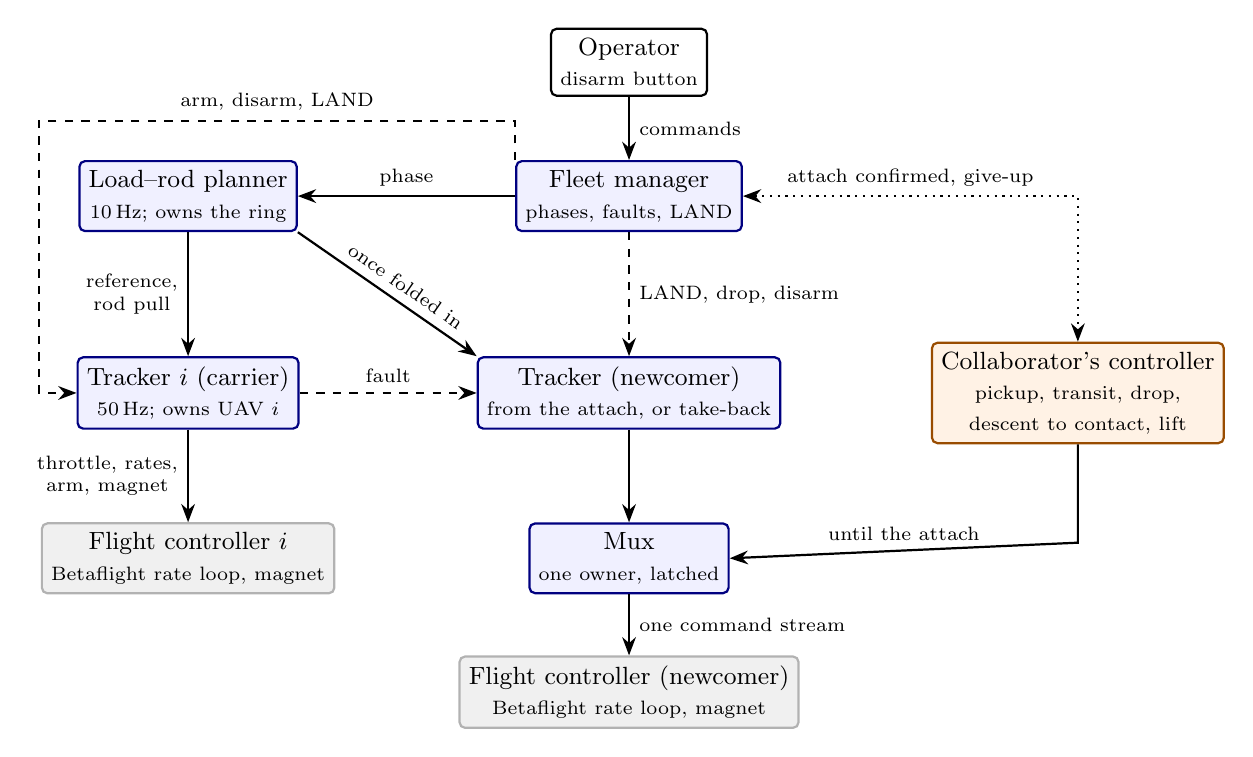
\begin{tikzpicture}[>=Stealth, font=\small,
    blk/.style={draw, thick, rounded corners=2pt, align=center, minimum height=0.85cm, font=\small},
    ours/.style={blk, fill=blue!6, draw=blue!50!black},
    his/.style={blk, fill=orange!10, draw=orange!60!black},
    fc/.style={blk, fill=gray!12, draw=gray!60},
    lab/.style={font=\scriptsize, align=center}]
  \node[blk]  (op)   at (5.6,1.7)   {Operator\\ \scriptsize disarm button};
  \node[ours] (fm)   at (5.6,0)     {Fleet manager\\ \scriptsize phases, faults, LAND};
  \node[ours] (plan) at (0,0)       {Load--rod planner\\ \scriptsize 10\,Hz; owns the ring};
  \node[ours] (trk)  at (0,-2.5)    {Tracker $i$ (carrier)\\ \scriptsize 50\,Hz; owns UAV $i$};
  \node[ours] (trkn) at (5.6,-2.5)  {Tracker (newcomer)\\ \scriptsize from the attach, or take-back};
  \node[his]  (tej)  at (11.3,-2.5) {Collaborator's controller\\ \scriptsize pickup, transit, drop,\\ \scriptsize descent to contact, lift};
  \node[ours] (mux)  at (5.6,-4.6)  {Mux\\ \scriptsize one owner, latched};
  \node[fc]   (bf)   at (0,-4.6)    {Flight controller $i$\\ \scriptsize Betaflight rate loop, magnet};
  \node[fc]   (bfn)  at (5.6,-6.3)  {Flight controller (newcomer)\\ \scriptsize Betaflight rate loop, magnet};
  \draw[->, thick] (op) -- node[lab, right] {commands} (fm);
  \draw[->, thick] (fm) -- node[lab, above] {phase} (plan);
  \draw[->, thick] (plan) -- node[lab, left] {reference,\\ rod pull} (trk);
  \draw[->, thick] (plan.south east) -- node[lab, sloped, above, pos=0.55] {once folded in} (trkn.north west);
  \draw[->, thick] (trk) -- node[lab, left] {throttle, rates,\\ arm, magnet} (bf);
  \draw[->, thick] (trkn) -- (mux);
  \draw[->, thick] (tej.south) -- ++(0,-1.25) -- node[lab, above] {until the attach} (mux.east);
  \draw[->, thick] (mux) -- node[lab, right] {one command stream} (bfn);
  \draw[->, thick, dashed] (trk) -- node[lab, above] {fault} (trkn);
  \draw[->, thick, dashed] (fm) -- node[lab, right] {LAND, drop, disarm} (trkn);
  \draw[->, thick, dashed] (fm.north west) -- ++(0,0.5) -| node[lab, pos=0.25, above] {arm, disarm, LAND} ([xshift=-0.5cm]plan.north west) |- (trk.west);
  \draw[<->, thick, dotted] (fm.east) -| node[lab, pos=0.25, above] {attach confirmed, give-up} (tej.north);
\end{tikzpicture}
\caption[The cascade and its owners]{The cascade and its owners. Blue: this work; orange: the collaborator's
controller; grey: the unmodified flight controllers. The planner owns the ring and the carriers' references; each
tracker owns one UAV's radio link; the newcomer's link is owned by the collaborator's controller until the attach
is confirmed and by this work's tracker from that tick, through a multiplexer that latches. Dashed: faults and the
fleet manager's commands; dotted: the confirmation and the give-up exchanged with the collaborator's stack. The
operator's disarm overrides everything.}
\label{fig:owners}
\end{figure}

\paragraph{The envelope and the fleet disarm.} Every tracker checks its own UAV against a flight envelope (UAV tilt
and ring tilt both 60$^\circ$, speed 3\,m/s) and checks that its motion-capture pose (0.25\,s) and the planner's
reference (1\,s) are fresh. A violation on a carrier disarms the whole fleet, not the one UAV: a single UAV losing
thrust on a shared rigid payload drags the others with it, and three UAVs cannot hold a ring hung for four. There
is no geofence. The argument for a fleet disarm rather than a geofenced recovery is the lab itself: the ring flies
at 1\,m inside a 6\,$\times$\,6\,$\times$\,4\,m cage, so a falling ring is a short fall onto a padded floor, where an
armed UAV flying on a wrong reference is not. The exceptions are UAVs that are not on the ring. A fault on a
newcomer that is not yet attached disarms the newcomer alone and lands the fleet, and a UAV that has left the ring
is pushed down to its own resting height and disarmed alone (Section~\ref{sec:reconfig}). LAND lands every UAV,
whatever it is doing. On the rig each UAV must confirm that its flight controller is armed before the fleet takes
off, and a UAV that disarms between ARM and TAKEOFF grounds the fleet, since three UAVs lifting a ring sized for
four would drag it.

\paragraph{The fall-backs, as runtime assurance.} The planner and the admission chain are the high-performance
controllers of a Simplex-style arrangement (Section~\ref{sec:lit_switching}); the fall-backs are simple, each has
its own monitor, and each ends with every UAV owned and down.
\begin{itemize}
    \item \textbf{Take-back.} A newcomer whose contact proves nothing, or whose owner gives up, is taken over by this
    work's tracker, moved clear of the ring and landed by itself (Section~\ref{sec:reconfig}).
    \item \textbf{Tilt cut.} A newcomer whose tilt passes its limit while it is not carrying the ring has its motors
    cut, so that a UAV caught on the rim or on a rod does not drag the ring: [injection to disarm about 0.26\,s in
    the twin; the rig value and the false-cut count over the rig bags, Section~\ref{sec:sim_attach}].
    \item \textbf{LAND for every UAV.} LAND lands the carriers with the ring, a freed carrier where it is, and a
    newcomer wherever it is in its mission, each on its own path down.
    \item \textbf{Landing the fleet on a newcomer fault.} A fault on an unattached newcomer disarms it alone and
    lands the carriers at once, where the earlier rule disarmed all four in the air.
    \item \textbf{Dropping the ring.} A second loss, or a ring tilt over 30$^\circ$, releases every magnet and lands
    every UAV: 30$^\circ$ is where the controller gives up a ring it can no longer hold level, not a value to design
    to (Section~\ref{sec:metrics}).
    \item \textbf{The freed UAV disarmed alone.} A carrier that has left the ring lands by itself and is disarmed at
    its rest without waiting for the fleet, so that the fleet's disarm at the end of a landing never drops it.
\end{itemize}

\paragraph{What is tested where.} ``A tested way down in every phase'' holds in the twin, where every fall-back
above has been flown from the phase it guards (Section~\ref{sec:sim_attach}). On the rig it holds only for the exits
flown there, and the rig switches are set per lab day: [the newcomer's warm tracker through a fault is a candidate
for the 21--22 October launch after its reviewer; the tilt cut and the flight controller's own disarm-to-land stay
off until 28--29 October, so that until then a take-back that sticks ends in a disarm from height; the model
integral through a resize and the freed UAV disarmed alone fly on 14 October]. Redistribution after a release has
flown on the rig; the policy for a true fault on a carrier stays the fleet stop and the drop rule. The
fault-coverage matrix, one row per fault and phase and one column per code tree, is [Appendix~\ref{sec:app_tests},
filled with the results].


\subsection{Method and metrics}
\label{sec:experiments}

Every result is flown against a named baseline, in the rig twin first and on the rig after it, under a rule
written before the runs. The parameters of the twin and of the rig are listed in Appendix~\ref{sec:app_params}.

% simulation.tex -- Methodology: simulation and verification (draft 4 Oct 2026).
% Sources: simulation_assets/ (generate_rigid_world.py, rig-twin worlds), simulation_communication
% (sim Betaflight bridges, rate_pid, imu_world), tools/sil/ (plant, lockstep), tools/run_experiment.py,
% results/registry.csv (832 rows on 4 Oct; run folders R0001-R0986 since 5 Aug), CURRENT_STATE 10.
% Counts: 667 unit tests in this work's packages and tools (4 Oct), excluding the collaborator's.
% Restructured 9 Oct (structure audit): now part of the experimental method; the list of simulator
% artefacts moved to the discussion (Section 4.6), the void rule stays; the SIL bench is defined here;
% the hardware test ladder moved here from hardware.tex.

\subsubsection{Rig twin and experiment runner}
\label{sec:simulation}

Every controller change is tested in simulation before it reaches the rig. The same launch files
and controller code run in simulation and on the rig.

\paragraph{Gazebo rig twin.} The physics simulator is Gazebo \cite{koenig2004gazebo}, connected to
ROS~2 \cite{macenski2022ros2} through bridges. The worlds are generated by a script from the lab's
measured geometry: the 0.86\,kg ring with its twelve plates, UAVs of 0.55\,kg, rods of 0.55\,m and
0.075\,kg with ball joints at both ends, pivoting 4\,cm below each UAV's centre. Each flight starts
with the ring on the floor. A flight controller emulator stands in for Betaflight. It maps the
throttle to rotor speed so that thrust follows the rig's identified affine map, with each UAV's own
offset and a battery that sags under load. It closes a proportional--integral rate loop on the
simulated gyro. A motion-capture emulator publishes the simulated poses on the rig's topics at
120\,Hz.

Wall-clock watchdogs fire when the simulation runs slower than real time, which it does (about 0.3
of real time with the full stack on the laptop); such runs are voided and flown again. The simulator
effects that had to be removed before the twin could be trusted are discussed in
Section~\ref{sec:discussion}. A software-in-the-loop (SIL) bench flies the same controllers against a
simulated plant that matches the controller's own model.

\paragraph{Experiment runner.} A run is described by a configuration file: the world, the launch
arguments, a timed list of events (ARM, TAKEOFF, wait for the lift, a push on the payload, DETACH,
ATTACH, LAND) and the pass/fail criteria. The runner starts from a clean machine, flies the run
headless, reads back the parameters every node actually loaded, and computes the metrics of
Section~\ref{sec:metrics} from the logs. About a thousand simulation runs were flown between August
and early October 2026.

\paragraph{Process.} Each experiment changes one variable against a named baseline run, and the
result it is expected to give is set out before it is flown. Every run is recorded with its
configuration, the variable changed, the baseline, the metrics and the outcome, including runs that
failed or were voided. Cases are flown twice; the tables give the number of runs in brackets, so (1)
marks a single run. Changes climb a ladder from cheapest to most
expensive: unit tests (about 670), a quick check script, headless Gazebo, and only then the rig.

\paragraph{Test ladder.} New behaviour is flown in an order that isolates one effect at a time:
free hover, to check the thrust map; then the payload held at its lift height; hover; the circle and
the figure-8; the detach; and the attach last. Each step is first flown in the rig twin with the
same launch commands.


% trajectories.tex -- Methodology: payload trajectories and computation (draft 4 Oct 2026).
% Definitions: mpc_planner/load_trajectory.py. Solve times measured from the planner logs
% (solve_ms column): rig 1 Oct flights h5_z100_rot120, c1_z100, f8_z100 (three UAVs, laptop,
% no Gazebo); Gazebo R0978/R0979 (three UAVs), R0931/R0935 (four UAVs), laptop at RTF ~0.3.

\subsection{Payload trajectories}
\label{sec:trajectories}

The payload reference is the lift schedule in height plus a horizontal offset from a trajectory.
The offset starts once the lift has reached the target height, and is applied to the whole formation,
so the UAVs keep their places around the payload. The planner evaluates the trajectory at the time
of every horizon node, so the plan sees the next two seconds of the path. The acceleration
$\mathbf{a}_L^{\mathrm{ref}}$ used for the cable references (Section~\ref{sec:controller}) is
its analytic second derivative.

Trajectories that start and end at rest use a smootherstep sweep of the path angle,
\begin{equation}
    \theta(t) = 2\pi\, s\!\left(\tfrac{t}{T}\right), \qquad s(u) = 6u^5 - 15u^4 + 10u^3, \quad u \in [0,1],
\end{equation}
whose first and second derivatives vanish at both ends, so the manoeuvre has no step in velocity or
acceleration that the suspended payload would take as a kick. The duration $T$ is chosen so that the
peak tangential speed equals the commanded speed $v$. The kinds are:
\begin{description}
    \item[Hover.] No horizontal motion; the payload holds the target height until LAND.
    \item[Line.] A shuttle along $x$, $\Delta x = \tfrac{d}{2}\left(1 - \cos\tfrac{2vt}{d}\right)$, repeated until LAND.
    \item[Circle.] One lap, $\Delta x = r\sin\theta$, $\Delta y = r(1-\cos\theta)$, with
    $T = 1.875 \cdot 2\pi r / v$. It starts at the lift point heading $+x$ and ends there at rest.
    \item[Figure-eight.] One Gerono lemniscate, $\Delta x = a\sin\theta$, $\Delta y = \tfrac{a}{2}\sin 2\theta$,
    with $T = 1.875 \cdot 2\pi a\sqrt{2} / v$ (the peak speed is at the crossing).
    \item[Spin.] The circle with one full turn of the payload's yaw, synchronised with the path.
    \item[Orbit.] The circle flown continuously at constant speed until LAND. The angular rate
    $v/r$ is reached through a smootherstep ramp over 4\,s, and the angle is its exact integral,
    so position, velocity and acceleration are continuous. The orbit keeps the payload moving
    for as long as a reconfiguration takes.
\end{description}

The results use an orbit of radius 0.5\,m at 0.125\,m/s (one lap in 25\,s) and a figure-eight of
$a = 1.0$\,m at 0.25\,m/s (67\,s, a $2 \times 1$\,m path), sized for the 6\,$\times$\,6\,m flight area
with the UAVs about 0.7\,m outside the payload's path.

\paragraph{Computation.} Both levels run on the same laptop as the motion-capture and radio nodes.
Table~\ref{tab:solve_times} gives the planner's solve time per tick. On the rig, with three UAVs,
the median is 24--30\,ms and the 95th percentile 49--55\,ms, inside the 60\,ms budget and the
100\,ms tick. In Gazebo the same laptop also runs the physics and the simulated sensors, which slows
the solves, but the simulation runs at about 0.3 of real time, so the planner still meets its tick in
simulated time. The four-UAV planner has not yet been timed on the rig.

\begin{table}[h]
\centering
\caption{Planner solve time per 10\,Hz tick (wall clock, one laptop).}
\label{tab:solve_times}
\begin{tabular}{llccc}
\toprule
Platform & Case & Median (ms) & 95th pct. (ms) & Max (ms) \\
\midrule
Rig, 3 UAVs & hover at 1.0\,m & 30.4 & 54.9 & 73.3 \\
            & orbit & 24.6 & 51.9 & 71.8 \\
            & figure-eight & 23.8 & 49.3 & 76.6 \\
\midrule
Gazebo, 3 UAVs & hover at 1.0\,m & 46.7 & 97.8 & 137.9 \\
               & orbit & 47.1 & 91.0 & 149.6 \\
Gazebo, 4 UAVs & hover at 1.0\,m & 118.5 & 193.2 & 298.5 \\
               & figure-eight & 106.2 & 189.1 & 313.7 \\
\bottomrule
\end{tabular}
\end{table}


% metrics.tex -- Methodology: metrics (draft 4 Oct 2026). The definitions are the ones used by the
% analysis tools (multi_drone_control/tools/method_metrics.py, push_metrics.py).
% 9 Oct (structure audit): the unused "carried fraction" metric cut; "every Gazebo case is flown at
% least twice" replaced, since several cells are single runs (marked (1)).

\subsubsection{Metrics}
\label{sec:metrics}

All metrics are computed from the logged motion-capture poses of the payload and the UAVs, with the
events (TAKEOFF, the push, DETACH, LAND) from the run's event log.
\begin{description}
    \item[Height error] $e_z = z_L - z_L^{\mathrm{ref}}$, positive with the payload high; in hover, averaged
    over the 15\,s before LAND. \textbf{Heave:} its peak-to-peak over the hover window.
    \item[Horizontal error] $\|\mathbf{e}_{xy}\|$, the horizontal distance between the payload's centre and
    its reference; on a trajectory, its mean over the first lap or the whole figure, and its maximum.
    \item[Payload tilt] The angle between the ring's axis and the vertical: its mean over the hover and its
    peak after an event.
    \item[Disturbance response] For a constant force applied for a fixed time, the displacement along the
    force relative to its mean over the 5\,s before: steady (mean over the last 5\,s of the force), peak
    (while the force acts), overshoot (the largest excursion the other way after it ends) and time to
    recover (after which it stays within 1\,cm). \textbf{Stiffness:} the force over the steady displacement
    with no integral action.
% SETTLED 10 Oct (was a CHECK): aligned with what Table tab:detach and Figure fig:detach measure
% (tools/thesis_sim_tables.py detach_stats, multi_drone_control): peak in the 5 s after DETACH; back in
% band = the tilt stays under the hover's own maximum over the 5 s before plus 0.5 deg; height change =
% largest |z - mean of the 5 s before| in the 12 s after. Was: "the time until the tilt stays under
% 2 deg, and the payload's height loss" (the pre-twin layout study's wording).
    \item[Detach] The peak payload tilt in the 5\,s after DETACH; the time until the tilt stays under
    the hover's own maximum over the 5\,s before DETACH plus 0.5$^\circ$ (back in band); and the largest
    change of the payload's height from its mean over the 5\,s before, in the 12\,s after. On the rig, where
    the ring rocks in hover, the rise of the peak above its mean over the 3\,s before the release is also
    given.
    \item[Attach] The peak payload tilt and the height loss (dip) after the weld, and whether the tilt
    returns under 2$^\circ$ within 3\,s; for the rejoin mission, also the tilt at the detach, the mean tilt
    over the orbit and the time from TAKEOFF to landed.
    \item[Solver health] The number of planner solves that failed or did not converge.
\end{description}
Each table cell is the mean over its runs, with the number of runs in brackets.

% 11 Oct: the physical rationale for the bars (health check, item 3). The metric definitions themselves (the
% tilt-vector rise over a 5 s pre-window, the post-event band, event times) are frozen on Mon 12 per the thesis
% plan's T6 (P1, D4) and replace the detach item above once signed.
\paragraph{Why these bars.} Three physical limits say what a transient may do to the ring, and the bars of the
results sections sit inside them. The first is the magnets. A plate holds its magnet straight off the face by
about 9--10\,N and by less under shear, so a tilt that turns a rod's pull across its plate can let a magnet go:
every ring lost on the rig began with an uncommanded magnet release, all of them with the rods planned at
45$^\circ$, and the rods are planned at 60$^\circ$ since 7 October so that each pull stays closer to its plate's
axis (Section~\ref{sec:sim_detach}). [The hold against the angle of pull, measured with a spring scale at 0, 30,
45 and 60$^\circ$ off the axis on 14 October, gives this limit its number.] The second is the fleet's own rule:
a ring tilt over 30$^\circ$, or a second loss, drops the ring and lands every UAV (Section~\ref{sec:safety}), so
30$^\circ$ is where the controller gives up, not a value to design to. The third is the model: the planner's
load--rod model and each tracker's rod pull assume a near-level ring, so a transient that stays within a few
degrees stays inside the regime the plan was computed for, and a transient that leaves it is being flown on a
plan that no longer describes the ring. The bars are therefore stated as a rise above the ring's own motion
before the event, small against the first two limits and inside the third, and every run is reported with its
measured rise so that a run that misses a bar is still read against the limits rather than against a number.



\newpage
\section{Results and Discussion}

% From the outline: every result is a table (2 repeats, named baseline) or a figure, then one
% paragraph of discussion. No run ids in the text; they are in the LaTeX comments and in
% configs/thesis_figures.yaml / docs/figures/PROVENANCE.md in the code repository.

% sim_results.tex -- draft of the simulation results (4 Oct 2026).
% Tables are generated by multi_drone_control/tools/thesis_sim_tables.py into Source/src/tables/,
% figures by tools/thesis_sim_figures.py (Images/*.pdf). Run ids: configs/thesis_figures.yaml.
% Cells give the mean over repeats with the number of runs in brackets.

\subsection{Carrying the payload in simulation}
\label{sec:sim_results}

The simulator is the Gazebo rig twin (Section~\ref{sec:simulation}), which reproduces the lab
set-up. It has a 0.86\,kg ring with its magnets at a radius of 0.225\,m, and 0.55\,kg UAVs on
0.55\,m rods of 0.075\,kg that pivot 4\,cm below each airframe. Thrust follows the rig's identified
affine map with battery sag, and the flight controller is a rate loop. Every flight starts
with the ring on the floor. The UAVs take off, swing their rods up to 45$^\circ$, pretension them
and lift the ring to 1.0\,m. Cases are flown twice; the tables give the number of runs in
brackets, so (1) marks a single run.

The height error is $e_z = z_L - z_L^{\mathrm{ref}}$, positive with the ring high, averaged over the
hover. The horizontal error $\|\mathbf{e}_{xy}\|$ is averaged over the first lap of a trajectory. For a
push, the displacement is measured along the push, relative to the mean over the 5\,s before it.

\subsubsection{Tracker initial condition}

Figure~\ref{fig:tracker_x0} and Table~\ref{tab:x0} compare the tracker's relaxed initial condition
($\epsilon = 0.025$) with node~0 pinned to the measurement ($\epsilon = 0$), both without integral
action.

\begin{figure}[h]
\centering
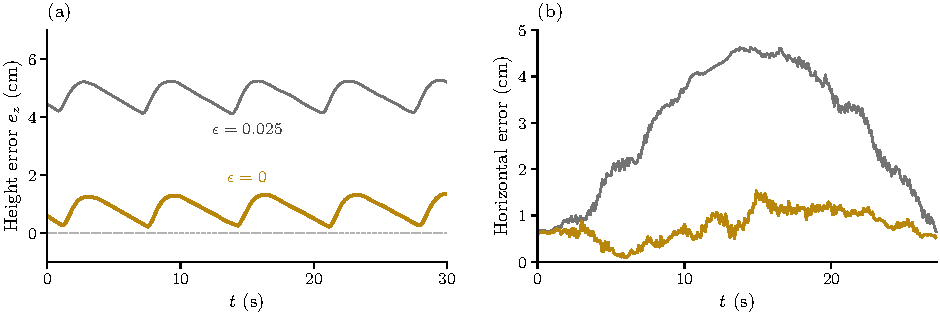
\includegraphics[width=\textwidth]{Images/tracker_x0.pdf}
\caption[Effect of the tracker's initial condition]{Effect of the tracker's initial condition without integral action: node~0 pinned to the
measured state ($\epsilon = 0$, gold) against the relaxed box ($\epsilon = 0.025$, grey). Gazebo rig
twin from a floor start, three UAVs. (a) Hover at 1.0\,m: ring height error from 10\,s after the
lift. Both settings show the same 1\,cm, 7\,s heave. (b) Circle of radius 0.5\,m at 0.125\,m/s:
horizontal ring error over the first lap including its 4\,s spin-up, sampled when the planner's
reference updates (10\,Hz). Dashed in (a): zero error. One run of each case is shown;
Table~\ref{tab:x0} gives the means.}
\label{fig:tracker_x0}
\end{figure}

\begin{table}[h]
\centering
\caption{Ring error with the relaxed and the pinned initial condition, no integral action. The
circle with $\epsilon = 0.025$ is a single run on an earlier code version; its horizontal error
reproduces on the current code (2.8\,cm, with the height integral on).}
\label{tab:x0}
% generated by tools/thesis_sim_tables.py
\begin{tabular}{llcc}
\toprule
Case & Metric & $\epsilon = 0.025$ & $\epsilon = 0$ \\
\midrule
Gazebo, hover at 1.0\,m & height error (cm) & +4.8 (2) & +0.9 (2) \\
Gazebo, circle & horizontal error, mean (cm) & 2.8 (1) & 0.8 (2) \\
 & height error (cm) & +4.8 (1) & +0.8 (2) \\
\bottomrule
\end{tabular}

\end{table}

With the box, each tracker could start its prediction from any state within 2.5\,\% of the
measured one. The solver used that freedom to treat its UAV as closer to the reference than it
was, so small errors were not corrected. Pinning node~0 brings the offset to under 1\,cm. The
remainder is attributed to
the rods' 0.075\,kg mass, which the planner does not model: they hold 52$^\circ$ instead of the
planned 45$^\circ$. This is not yet tested with node~0 pinned. With the box in place, adding the
rods' mass to the planner's model corrected the rod elevation but did not move the height.

\redo{the relaxed box against node~0 pinned on a plant that matches the controller's model (the software-in-the-loop bench, once it flies the twin), three UAVs, hover: whether the box is the whole of the height offset, and whether the rods then hold the planned 45$^\circ$ and tension.}
% --- original text, flown before the rig twin; kept to refill this place:
% With the box, each tracker could start its prediction from any state within 2.5\,\% of the
% measured one. The solver used that freedom to treat its UAV as closer to the reference than it
% was, so small errors were not corrected. In SIL, where the plant matches the model, this was the
% whole of the payload's height offset. Pinning node~0 removes it, and the rods hold the planned
% 45$^\circ$ and the planned tension. In Gazebo the offset drops to under 1\,cm. The remainder is attributed to

The box was a fraction of each \emph{absolute} coordinate, so it widened as the UAVs moved away from
the world origin. The circle's error with the box grows with the ring's distance from the origin,
which is consistent with this (Figure~\ref{fig:tracker_x0}b), although on this circle the distance and
the phase of the lap change together. Pinning node~0 also removes most of that error.

Landing is not yet resolved, with or without the box. In 21 Gazebo flights with $\epsilon = 0$, one
UAV tipped over during landing after the payload had touched down, as 2 of 32 earlier landings with the
box had. Both come from landing, not from the box, and the landing of Section~\ref{sec:sim_landing}
removes them.

\subsubsection{Disturbance rejection}

A constant force was applied to the ring for 15\,s in hover: 0.6\,N downward, about the weight of a
60\,g object, and 0.4\,N horizontally. Both were sized so that the integral stays inside its
bound, at 56\,\% and 51\,\% of it. Without an integral the ring settles 8.4\,cm and 7.6\,cm away, which gives the closed loop's
stiffness to a force on the ring: $K_z = 7.1$\,N/m and $K_{xy} = 5.3$\,N/m, the values used for
$K$ in \eqref{eq:lumped_int}. Figure~\ref{fig:disturbance} shows the model integral on the horizontal push, and
Table~\ref{tab:disturbance} gives both pushes and compares it with the target-shift form.

\begin{figure}[h]
\centering
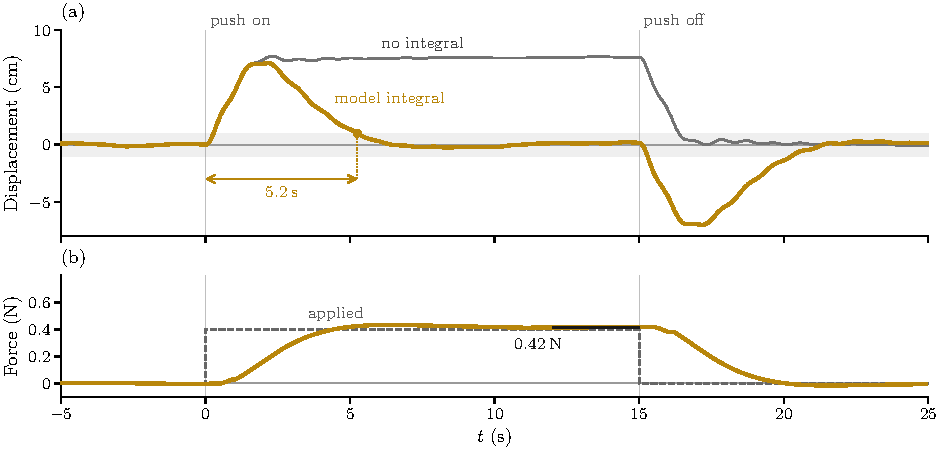
\includegraphics[width=\textwidth]{Images/disturbance.pdf}
\caption[Rejection of a constant force on the ring]{Rejection of a constant force on the ring, Gazebo rig twin, three UAVs, hover at 1.0\,m.
A 0.4\,N horizontal push acts from 0 to 15\,s. (a) Ring displacement along the push, relative to its
mean over the 5\,s before: no integral (grey) and the integral in the planner's model (gold). Band:
$\pm 1$\,cm. Arrow: time for the model integral to bring the ring back within 1\,cm for good. (b)
Change of the model integral's force $\mathbf{d}$ along the push from its value before the push
(gold), against the applied force (dashed). Black bar: its mean over the last 3\,s of the push. The
force holds still for about 0.7\,s after each step, while the ring moves faster than the integral's
5\,cm/s gate. One run of each case is shown; Table~\ref{tab:disturbance} gives the means and the
0.6\,N vertical push.}
\label{fig:disturbance}
\end{figure}

\begin{table}[h]
\centering
\caption{Disturbance rejection in the Gazebo rig twin with $\epsilon = 0$. One of the two
target-shift runs aborted on landing, after the push and its recovery; its push is included. The
change of the integral force is measured from its value before the push (0.06\,N vertically,
0.03\,N horizontally).}
\label{tab:disturbance}
% generated by tools/thesis_sim_tables.py
\small
\begin{tabular}{lccc}
\toprule
 & No integral & Target shift & Model integral \\
\midrule
\multicolumn{4}{l}{\emph{0.6\,N downward push on the ring}} \\
\quad steady displacement (cm) & 8.4 (2) & 0.3 (2) & 0.2 (2) \\
\quad peak displacement (cm) & 8.9 (2) & 6.6 (2) & 6.5 (2) \\
\quad overshoot on release (cm) & 0.4 (2) & 7.1 (2) & 7.0 (2) \\
\quad time to within 1\,cm after onset (s) & -- & 6.0 (2) & 6.1 (2) \\
\quad change of the integral force (N) & -- & -- & 0.58 (2) \\
\midrule
\multicolumn{4}{l}{\emph{0.4\,N horizontal push on the ring}} \\
\quad steady displacement (cm) & 7.6 (2) & n/a & 0.1 (2) \\
\quad peak displacement (cm) & 7.7 (2) & n/a & 7.2 (2) \\
\quad overshoot on release (cm) & 0.1 (2) & n/a & 7.0 (2) \\
\quad time to within 1\,cm after onset (s) & -- & n/a & 5.5 (2) \\
\quad change of the integral force (N) & -- & n/a & 0.42 (2) \\
\midrule
\multicolumn{4}{l}{\emph{One UAV producing more thrust than its map assumes}} \\
\quad height error (cm) & -- & 0.0 (2) & 0.0 (2) \\
\quad horizontal error (cm) & -- & 3.5 (2) & 0.0 (2) \\
\quad ring tilt (\si{\degree}) & -- & 6.4 (2) & 7.9 (2) \\
\bottomrule
\end{tabular}

\end{table}

Both forms of the integral bring the ring back to the target, and on the vertical push their
transients are the same to within a few per cent. With the conversion $K$ set to the measured
stiffness, the loop has the same gain whether the integral moves the target or enters the model. The
force the model integral learns is the force that was applied, within 3\,\% vertically and
4--5\,\% horizontally. Only the model form
acts horizontally, and it removes the horizontal push in the same way.

The integral reduces the peak only partly, by about a quarter vertically (8.9 to 6.5\,cm) and by
7\,\% horizontally (7.7 to 7.2\,cm), because it is slower than the cascade. The ring reaches most
of its uncompensated displacement within about 1\,s, while the integral's time constant is
$1/k_i = 2.5$\,s. When the push ends, the integral still holds the force it learned and drives the
ring past the target by about as much as the push displaced it at onset. This overshoot on release
is a property of integral action, not of where the integral acts. Table~\ref{tab:gain} shows the
trade-off. Doubling $k_i$ reduces the peak by 14\,\%, but the response rings and settles 55\,\% later,
the trend the damping relation of Section~\ref{sec:disturbance} predicts. This is a single run, and its
settling time is sensitive to the 1\,cm threshold against the 1\,cm heave of the hover. Keeping the
ring-speed gate only for the first 5\,s after the lift removes 7--8\,\% with no cost on this push; it has
not yet been flown on a trajectory, a hand-over or a landing.

\begin{table}[h]
\centering
\caption{Integral gain and gate on the 0.6\,N vertical push, model integral. Peak: largest
displacement during the push; overshoot and settling (to within 1\,cm): after it ends. Brackets:
number of runs.}
\label{tab:gain}
% generated by tools/thesis_sim_tables.py
\begin{tabularx}{\textwidth}{Xccc}
\toprule
Model integral & Peak (cm) & Overshoot (cm) & Settling (s) \\
\midrule
$k_i = 0.4$ & 6.5 (2) & 7.0 (2) & 4.7 (2) \\
$k_i = 0.8$ & 5.6 (1) & 6.0 (1) & 7.2 (1) \\
$k_i = 0.4$, speed gate only in the first 5\,s after the lift & 6.0 (1) & 6.4 (1) & 4.5 (1) \\
\bottomrule
\end{tabularx}

\end{table}

When one UAV produces more thrust than its map assumes, both forms hold the height. Only the model
form also removes the horizontal error, and the ring tilts 1.5$^\circ$ further. The thrust error is a
moment on the ring that neither form controls.

\redo{the two forms of the integral with the feedforward to the trackers scaled to 0.9, on a plant that matches the controller's model (the software-in-the-loop bench, once it flies the twin): the planned ring position half a second ahead against the actual one, the rod elevation, and how much of its bound the model integral uses.}
% --- original text, flown before the rig twin; kept to refill this place:
% In SIL the two forms can be compared directly, with the feedforward to the trackers scaled to 0.9.
% Both hold the target, but the reference-shift form raises the height target by 10\,cm and plans a
% climb towards it that never comes: the planned ring position half a second ahead is 4.2\,cm above
% where the ring is. The rods also settle at 48$^\circ$ rather than the planned 45$^\circ$. With the
% model integral the plan predicts what happens (0.0\,cm) and the rods hold 45$^\circ$. In SIL the model
% integral used 89\,\% of its vertical bound (0.95 of 1.07\,N) and raised its warning, because the
% conversion $K$ measured in Gazebo is lower than the SIL plant's stiffness.
% % TODO: generate the SIL plan-prediction numbers from the planner logs as the tables are.

\subsubsection{Other approaches to model error}
\label{sec:sim_methods}
% Sources: docs/overnight_2026-10-04.md (report table), registry R0841-R0955; notes 2026-10-03_*,
% 2026-10-04_* (offset_free_mpc = A, offset_free_innovation, indi_fext, kt_trim, pin_cable_rates,
% ancillary_tracker, l1_ring, xy_stiffness_b3); B4 notes 2026-10-01_load_ext_force (offline replay).
% All flown with the tracker box at 0.025 (before the x0 finding): the +4.8 cm hold is the box.

Before the initial-condition fix, several approaches from the literature were tried against the
steady errors, and each was tested in the same three-UAV rig twin. Three
cases represent the internal errors: the hover itself, and one UAV whose thrust map is wrong in
each direction (its real offset 0.03 above or below the 0.185 its tracker assumes). Two represent
external forces: a 1\,N horizontal push on the ring, and a 0.4\,m/s wind during the orbit.
Table~\ref{tab:methods} gives the results. All of them were flown with the tracker's relaxed initial
condition, so the hover without any correction sits 4.8\,cm high; the comparisons between rows still
hold.

\begin{table}[h]
\centering
\footnotesize
\setlength{\tabcolsep}{4pt}
\caption{Approaches to model error in the Gazebo rig twin (three UAVs, 1.0\,m, floor start; flown
with $\epsilon = 0.025$). Height and horizontal errors in cm, tilt in degrees; one run per cell
unless noted; a dash: not flown. $^{a}$ A UAV tipped during the landing, after the hover, and the fleet
disarmed. $^{b}$ Two runs, agreeing within 0.1.}
\label{tab:methods}
\begin{tabular}{lccccc}
\toprule
 & Hover & One UAV weaker & One UAV stronger & 1\,N push & Wind \\
 & $e_z$ & $e_z$ / $e_{xy}$ / tilt & $e_z$ / $e_{xy}$ / tilt & $e_{xy}$ & $e_{xy}$ \\
\midrule
None & +4.8 & $-$3.0 / 3.8 / 6.7 & +12.8 / 3.5 / 6.0 & 18.0 & 17.9 \\
Height integral (target) & +0.1 & 0.0 / 3.8 / 6.7 & 0.0 / 3.5 / 6.0 & 17.9 & 18.0 \\
Force balance & +3.8 & +3.9 / 1.3 / 9.0 & -- & 0.3 & 3.9 \\
Force balance + height int. & +0.1$^{b}$ & 0.0 / 1.3 / 9.0$^{b}$ & -- & 0.4$^{b}$ & 3.9$^{b}$ \\
Offset-free observer & +1.6 & +1.0 / 0.2 / 8.0 & +2.4 / 0.1 / 7.5 & 2.6$^{b}$ & 7.8$^{b}$ \\
Measured cable force & +4.2$^{a}$ & +3.8 / 3.1 / 0.8$^{a}$ & +4.5 / 0.6 / 0.3 & -- & -- \\
Measured force + height int. & 0.0$^{a}$ & 0.0 / 3.1 / 0.8 & 0.0 / 0.6 / 0.3$^{a}$ & -- & -- \\
Thrust-gain trim & +3.7 & +4.1 / 1.3 / 2.3 & -- & -- & -- \\
Rod mass in the planner & +5.0 & -- & -- & -- & -- \\
\bottomrule
\end{tabular}
\end{table}

\begin{description}
    \item[Height integral on the target.] Zeroes the height in every case and does nothing
    horizontally: the push and the wind still move the ring 18\,cm.
    \item[Force balance.] Estimates a constant force on the ring and one shared by the UAVs from
    the measured motion and the delivered thrust, and gives them to the planner's model
    \cite{muske2002disturbance}. It removes the push and most of the wind. It cannot see the internal
    height offset: by Newton's law, a force that the system exerts on itself does not appear in its
    total. It books a UAV's thrust-map error as a force on the ring, and leans the formation into
    it, which tilts the ring further. Combined with the height integral it was the best on height and
    external forces. Its transients were not small: on the push it peaked at 14.5\,cm, and on release
    it overshot by 14.8\,cm and tilted the ring 7.1$^\circ$.
    \item[Offset-free observer.] Estimates the force from the planner's own prediction error, as in
    offset-free MPC \cite{pannocchia2003disturbance}. It helped everywhere but converged slowly and left
    residuals, because a small offset shows up in the plan's cable states rather than in the payload's
    predicted motion.
    \item[Measured cable force.] Each tracker takes the cable force from its measured acceleration
    and delivered thrust, the ground-side counterpart of the IMU-based compensation of
    \cite{tudelft}. It was the only approach that levelled the ring against one UAV's wrong thrust
    map (0.3--0.8$^\circ$ against 6--7$^\circ$), because it corrects each UAV's own force. In four of
    six runs, however, a UAV tipped during the landing.
    \item[Thrust-gain trim.] A per-UAV estimate of the throttle-to-acceleration gain, from the UAV's
    own measured acceleration and its static share of the cable force. It partly corrects a wrong map.
    \item[Rod mass in the planner.] Corrected the rods' elevation (49.7 to 42.8$^\circ$ against a planned
    45$^\circ$) but not the height.
\end{description}
Further candidates were rejected before flying, because tests on logged flights showed they would
not work. These were pinning the cable rates at node~0, a thrust reference weight in the
tracker, and an $\mathcal{L}_1$ adaptive force estimate \cite{hovakimyan2010l1} at the planner's
10\,Hz rate. Raising the planner's weight on the ring's horizontal position by three and by ten times
cut the push displacement only by 23 and 38\,\% (18.5 to 14.3 and 11.4\,cm), and the higher weight
rocked the ring by 6$^\circ$. Aiming the rods at the hand-over angle instead of 45$^\circ$ made it
worse (20.7\,cm). Both were removed.

Two conclusions carried forward. First, the internal height offset was not a force at all, which is
why no force estimate could find it; it turned out to be the tracker's initial condition.
Second, a wrong thrust map on one UAV is a moment on the ring, and only a correction of that UAV's own
force removes the tilt it causes. A force on the ring, estimated or integrated, can only move the
whole formation.

\subsubsection{Trajectories}

Table~\ref{tab:traj} gives the tracking of each reference kind of Section~\ref{sec:trajectories} in
the rig twin with $\epsilon = 0$, three or four UAVs from a floor start. The integral action was off,
so the height column is the static offset that the height integral removes
(Section~\ref{sec:disturbance}). The horizontal error stays about a centimetre on average and under
3\,cm at worst for every reference, with three UAVs or four. The spin turns the ring once about its
vertical axis while it circles, and the ring follows that yaw within a few degrees.

\begin{table}[htbp]
\centering
\caption[Trajectory tracking]{Trajectory tracking in the Gazebo rig twin, $\epsilon = 0$, no integral
action, ring at 1.0\,m, floor start. Four UAVs fly the even ring except in the four-UAV hover, which
uses the detach layout. Speed: the commanded speed, which the line and the spin reach at their
peak. Horizontal error per sample, sampled where the planner's reference updates, over the motion
(the circle's first lap) or the 15\,s before LAND (hover); height error and tilt: means over the
same window; each cell is the mean over the runs.}
\label{tab:traj}
% generated by tools/thesis_sim_tables.py
\begin{tabularx}{\textwidth}{>{\raggedright\arraybackslash}Xccccccc}
\toprule
 & & Speed & \multicolumn{2}{c}{Horizontal error (cm)} & Height & Tilt & \\
\cmidrule(lr){4-5}
Reference & UAVs & (m/s) & mean & max & error (cm) & (\si{\degree}) & Runs \\
\midrule
Hover & 3 & -- & 0.7 & 0.7 & $+$0.9 & 1.2 & 2 \\
Hover, plates 1/3/5/9 & 4 & -- & 0.6 & 0.7 & $-$2.2 & 1.6 & 2 \\
Line, 1\,m shuttle & 4 & 0.25 & 0.9 & 2.7 & $-$1.7 & 1.3 & 2 \\
Circle, $r = 0.5$\,m & 3 & 0.125 & 0.8 & 1.5 & $+$0.8 & 1.2 & 6 \\
Circle, $r = 0.5$\,m & 4 & 0.125 & 0.9 & 1.9 & $-$1.7 & 1.3 & 2 \\
Figure-8, 2\,m $\times$ 1\,m & 4 & 0.25 & 0.8 & 2.4 & $-$1.7 & 1.3 & 2 \\
Spin, circle with one turn of yaw$^a$ & 4 & 0.125 & 0.5 & 1.4 & $-$1.7 & 1.2 & 2 \\
\bottomrule
\multicolumn{8}{l}{\footnotesize $^a$ Yaw error 1.3\,\si{\degree} mean, 3.5\,\si{\degree} max over the turn.}
\end{tabularx}

\end{table}

The circle and the figure-8 were also flown with the relaxed box of
Section~\ref{sec:sim_results}, $\epsilon = 0.025$ (Figure~\ref{fig:traj}). Pinning node~0 cut the
horizontal error over the motion from 3.0 to 1.0\,cm on the circle and from 2.9 to 0.8\,cm on the
figure-8, and the height error from $+3.2$ to $-1.7$\,cm. The relaxed box's error grows as the ring
moves away from the world origin and shrinks as it returns, in both shapes.

\begin{figure}[h]
\centering
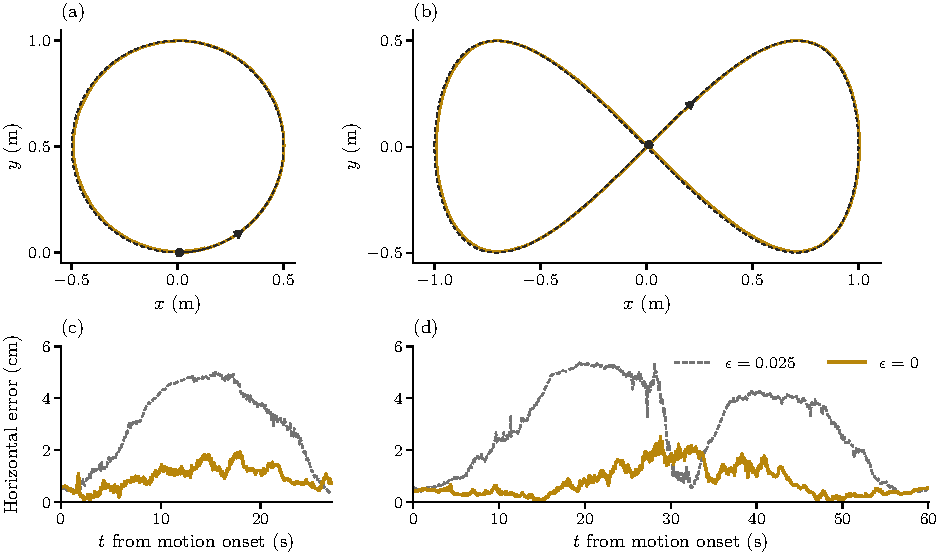
\includegraphics[width=\textwidth]{Images/trajectories.pdf}
\caption[Trajectory tracking with four UAVs]{Pinning node~0 cuts the four-UAV trajectory error by about
a factor of three. (a) Circle of radius 0.5\,m, one lap of 27\,s including a 4\,s spin-up; (b) a
2\,m\,$\times$\,1\,m figure-8 in 60\,s. Gold: ring path with $\epsilon = 0$; dark dashed: reference;
dot and arrow: start and direction. (c, d) Horizontal ring error from the onset of motion, sampled
when the planner's 10\,Hz reference updates, with $\epsilon = 0$ (gold) and the relaxed box
($\epsilon = 0.025$, dashed). Gazebo rig twin, four UAVs on the even ring, ring at 1.0\,m; one run of
each.}
\label{fig:traj}
\end{figure}

\subsubsection{Landing}
\label{sec:sim_landing}

Figure~\ref{fig:landing} compares a straight descent with the landing of
Section~\ref{sec:takeoff}, and Table~\ref{tab:land} gives every landing flown in the rig twin
with $\epsilon = 0$: three and four UAVs, hover, the pushes, the thrust-map errors, the circle and the
detach. With a straight descent, 2 of 21 landings tipped a UAV past 45$^\circ$. With the unwind alone
the outward push was gone but 2 of 18 still tipped: one survivor oscillated when the cable term
stepped off, and one departed UAV rocked on the floor. With the feedforward ramp and the ground idle
added, none of 18 tipped.

\begin{figure}[h]
\centering
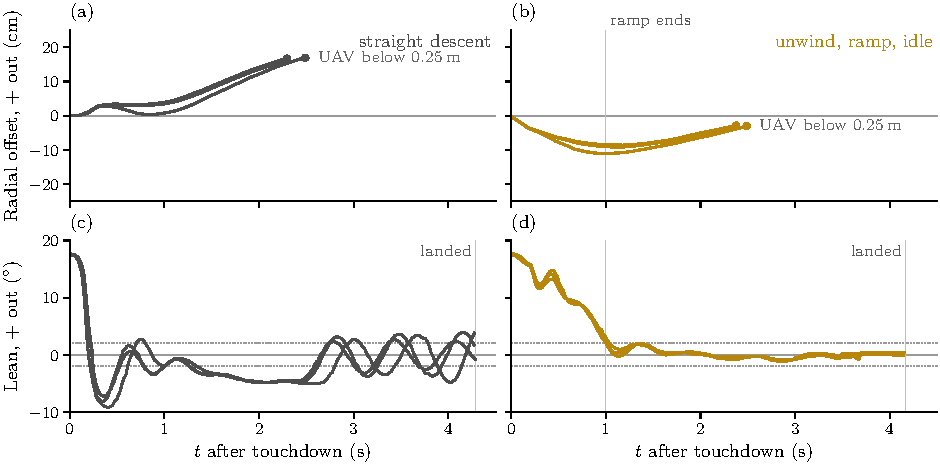
\includegraphics[width=\textwidth]{Images/landing.pdf}
\caption[Landing after touchdown]{Landing after the payload touches down, Gazebo rig twin, three
UAVs (interchangeable; one run of each). (a, c) Straight descent, with the cable feedforward cut at
touchdown. (b, d) Unwind along the rods, a 1\,s feedforward ramp and idle on the floor. (a, b) Radial
offset of each UAV from its reference about the ring centre, positive outward, drawn until the UAV
is below 0.25\,m (dot), below which its reference follows it. (c, d) Lean of each UAV's thrust axis
along its outward radial; the 17.5$^\circ$ at touchdown is the lean against the rod's pull. Dotted:
$\pm 2^\circ$. In a straight descent the rods push the UAVs outward, still growing at 17\,cm, and the
UAVs keep rocking until they land. With the unwind they trail their outward-moving reference instead
and settle within $\pm 2.6^\circ$ once the ramp ends.}
\label{fig:landing}
\end{figure}

\begin{table}[h]
\centering
\caption{Every landing in the Gazebo rig twin with $\epsilon = 0$, from load-down until the fleet is
declared landed. Tipped: a UAV past 45$^\circ$; the fleet aborts at 60$^\circ$. The ranges are over
the landings without a tip.}
\label{tab:land}
% generated by tools/thesis_sim_tables.py
\begin{tabularx}{\textwidth}{>{\raggedright\arraybackslash}Xcccc}
\toprule
Landing & Runs & Tipped (aborted) & Pushed outward (cm) & Tilt after 1.2\,s (\si{\degree}) \\
\midrule
straight descent & 21 & 2 (1) & 5.4--18.2 & 2.2--5.7 \\
unwind & 18 & 2 (2) & 0.5--4.1 & 2.4--5.0 \\
unwind, feedforward ramp, ground idle & 18 & 0 (0) & 0.5--3.0 & 1.8--4.0 \\
\bottomrule
\end{tabularx}

\end{table}



% sim_detach.tex -- Results: detach in simulation (draft 4 Oct 2026). No run ids in the text.
% Runs: OCP vs network R0111-R0114 (6 Aug, 0.4 kg payload, 0.5 m cables, circle 0.6 m/s);
% hand-back R0093 (even ring, 62 deg), R0108/R0109; SIL mode study R0496-R0505 (25 Sep);
% layout R0559-R0572 (hover) and R0554/R0556 (mid-circle) (25 Sep, legacy
% linear plant, 0.86 kg ring, 0.5 m rods, 0.64 kg UAVs); 1/3/6/9 R0582/R0584; LAND v4 R0571/R0572;
% rig twin W4 rehearsal R0939 (4 Oct, 0.55 m rods, 0.55 kg UAVs, affine map, old tracker box).
% Restructured 9 Oct (structure audit): opens with its question, baseline and bar; order layout,
% transient, against the network, rig; the freed UAV's own landing added (fig:departed_landing) with
% pending rig figures.

\subsection{Detach}
\label{sec:sim_detach}

This section answers the leave half of RQ1: does a detach by OCP resize keep the ring level when one UAV
of four leaves? The baseline is a hand-off of the payload to the dissipative network on the same
detach, and for the geometry the even layout; the bar is the ring's tilt back under the hover's own
maximum plus 0.5$^\circ$ (Table~\ref{tab:detach}).

\paragraph{Layout.}
\redo{detach layout study, four UAVs to three in hover, the UAV on plate~3 released, two runs per layout: the even ring (plates 0/3/6/9) against plates 1/3/5/9 (peak and settled tilt); the 1/3/5/9 detach in the middle of a circle; plates 1/3/6/9 (clearance of the departing UAV against tilt and throttle).}
% --- original text, flown before the rig twin; kept to refill this place:
% \paragraph{Layout.} The geometric condition of Section~\ref{sec:reconfig} was tested directly. Four
% UAVs on an even ring (plates 0/3/6/9) and on plates 1/3/5/9 hovered, and the UAV on plate~3 was
% released. On the even ring the three survivors' attachment points have the ring's centre of mass on
% the edge of their support triangle, and the payload swung to a 25.6--28.5$^\circ$ peak and settled at
% 6.7--6.8$^\circ$. On plates 1/3/5/9 the survivors form an even triangle: the peak was
% 3.0--3.3$^\circ$ and the payload settled at 0.1--0.2$^\circ$ (Table~\ref{tab:detach_layout}). The same
% detach in the middle of a circle peaked at 6.9--7.7$^\circ$ and settled at 0.3$^\circ$, and the
% survivors continued the circle. Moving one more UAV, to plates 1/3/6/9, gives the departing UAV more
% room (0.82\,m to its nearest neighbour instead of 0.58\,m) at a cost of 2.5$^\circ$ of peak tilt,
% 0.45$^\circ$ of settled tilt and 10\,\% more throttle on one survivor.
%
% \begin{table}[h]
% \centering
% \caption{Detach from four UAVs to three in hover, Gazebo, 0.86\,kg ring, by layout. Two runs per layout.}
% \label{tab:detach_layout}
% \begin{tabular}{lcc}
% \toprule
% Layout (plates) & Peak tilt after DETACH & Settled tilt \\
% \midrule
% Even, 0/3/6/9 & 25.6--28.5$^\circ$ & 6.7--6.8$^\circ$ \\
% 1/3/5/9 & 3.0--3.3$^\circ$ & 0.1--0.2$^\circ$ \\
% 1/3/5/9, mid-circle & 6.9--7.7$^\circ$ & 0.3$^\circ$ \\
% \bottomrule
% \end{tabular}
% \end{table}

\paragraph{The transient.} Figure~\ref{fig:detach} shows one detach in the rig twin: four UAVs on plates 1/3/5/9 in hover, the
UAV on plate~3 released, with $\epsilon = 0$. The uneven 1/3/5/9 layout loads the UAV on plate~9 most.
At DETACH the planner, re-solved for the three survivors on their actual plates, hands the released
UAV's load to them in one 0.1\,s tick. The ring tilts by at most 3.3$^\circ$ and is back within its
hover band after 1\,s.

\begin{figure}[h]
\centering
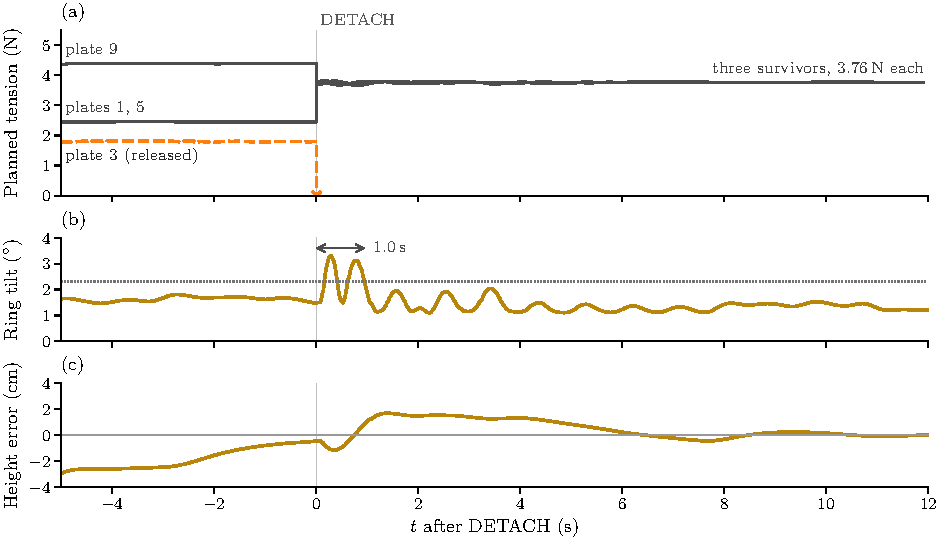
\includegraphics[width=\textwidth]{Images/detach.pdf}
\caption[Detach by OCP resize]{Detach of one UAV of four by OCP resize, Gazebo rig twin, hover at
1.0\,m, UAVs on plates 1, 3, 5 and 9 (Figure~\ref{fig:geometry}). (a) Rod tension planned for each
UAV; the UAV on plate~3 (dashed) is released at DETACH, and the three survivors, now an even
triangle, share the load equally. (b) Ring tilt; dotted: the hover's own maximum plus 0.5$^\circ$;
arrow: time until the tilt stays below it. (c) Ring height error against the 1.0\,m target. One run;
the tensions are planned, since the rig twin does not measure them.}
\label{fig:detach}
\end{figure}

\paragraph{Repeats.} Table~\ref{tab:detach} gives the same detach over five runs with $\epsilon = 0$,
against the earlier rehearsal, which differed in two ways: the relaxed box and the height integral on.
With $\epsilon = 0$ every run peaks at a few degrees and is back within its hover band in about a
second, and the five runs agree closely.

\begin{table}[htbp]
\centering
\caption[Detach, repeats]{Detach of one UAV of four in hover by OCP resize, Gazebo rig twin, plates 1,
3, 5 and 9, ring at 1.0\,m. Peak tilt: in the 5\,s after DETACH. Back in band: time until the tilt
stays under the hover's own maximum plus 0.5$^\circ$. Height change: largest change from the mean
height before DETACH, in the 12\,s after. Ranges over the runs.}
\label{tab:detach}
% generated by tools/thesis_sim_tables.py
\begin{tabularx}{\textwidth}{>{\raggedright\arraybackslash}Xcccc}
\toprule
 & & Peak tilt & Back in band & Height change \\
Tracker box & Runs & (\si{\degree}) & (s) & (cm) \\
\midrule
$\epsilon = 0.025$, height integral on & 1 & 3.2 & 2.6 & 2.7 \\
$\epsilon = 0$, no integral & 5 & 2.8--4.0 & 0.9--1.0 & 3.4--3.6 \\
\bottomrule
\end{tabularx}

\end{table}

\paragraph{OCP resize against network hand-off.}
\redo{OCP resize against network hand-off on the same detach, four UAVs to three during a circle (and in hover): settled payload tilt and the survivors' tracking error; with it the network's hand-back to the planner, with and without the two fixes (no soft-start restart on an airborne hand-back, solver primed before it flies).}
% --- original text, flown before the rig twin; kept to refill this place:
% \paragraph{OCP resize against network hand-off.} Table~\ref{tab:detach_ab} compares the two detach
% methods of Section~\ref{sec:reconfig} on the same flight: four UAVs flying a circle, one released
% mid-way. The flights used an early payload (0.4\,kg, 0.5\,m cables, circle at 0.6\,m/s). With the OCP
% resize the payload settled level and the survivors kept tracking their references. With the network
% hand-off the payload settled tilted by 26--48$^\circ$, and the survivors were 0.06--0.91\,m off their
% references while the network redistributed the load. Two fixes were needed for the network sequence
% to hand back to the planner at all: the feedforward soft-start must not restart on an airborne
% hand-back, and the new solver must be primed before it flies. Without them the payload dropped to
% 0.07\,m above the floor after the detach; with them it stayed above 0.46\,m.
%
% \begin{table}[h]
% \centering
% \caption{Detach from four UAVs to three during a circle, Gazebo, early payload (0.4\,kg).}
% \label{tab:detach_ab}
% \begin{tabular}{lcc}
% \toprule
%  & OCP resize & Network hand-off \\
% \midrule
% settled payload tilt & about 1$^\circ$ & 26--48$^\circ$ \\
% survivor tracking error & about 1\,mm & 60--910\,mm \\
% \bottomrule
% \end{tabular}
% \end{table}

\redo{the same comparison on a plant that matches the controller's model (the software-in-the-loop bench, once it flies the twin), hover and circle: payload tilt after the detach with the network against the OCP resize.}
% --- original text, flown before the rig twin; kept to refill this place:
% On the 0.86\,kg ring the gap widened. In the software-in-the-loop bench the network aborted the
% flight at 53--61$^\circ$ of payload tilt after a detach, both in hover and in the circle, while the
% OCP resize held the survivors level to within 0.5--2$^\circ$.

\paragraph{On the rig.} The detach was flown on the rig on 8 October, in four flights.
Figure~\ref{fig:rig_detach} sets their ring tilt and height error after the release against the twin.

\pendingfig{fig:rig_detach}{Detach on the rig against the twin: ring tilt and height error after the release for the announced, unannounced and 150-degree-gap detaches; rig gold, twin repeats grey.}{built from the 8 Oct rig runs (next)}

\paragraph{The freed UAV's own landing.} After a detach the freed UAV lands by itself, off the ring
(Section~\ref{sec:reconfig}). On the rig on 8 October this landing did not finish: in all four detach
flights the freed UAV floated above its resting height until the fleet's disarm at the end of the
landing dropped it about 0.3\,m (Figure~\ref{fig:departed_landing}a), and the twin shows the same stall
(Figure~\ref{fig:departed_landing}b). Its landing was therefore changed: its height reference is pushed
down to its own resting height, and once it is there it is disarmed alone, without waiting for the
fleet (Figure~\ref{fig:departed_landing}c, in the twin). Figure~\ref{fig:rig_departed} shows the
change on the rig.

\begin{figure}[htbp]
\centering
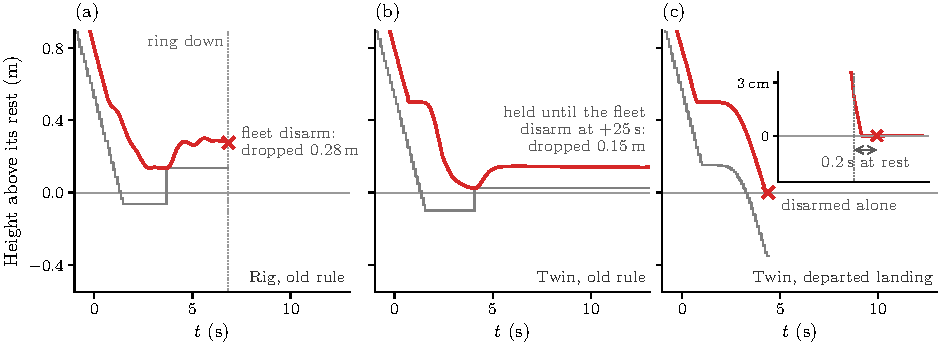
\includegraphics[width=\textwidth]{Images/departed_landing.pdf}
\caption[A freed UAV's own landing, old rule and departed landing]{A UAV landing by itself off the ring, the same UAV (QUAD4) in three cases, aligned where it passes 0.8\,m on the way down; solid: its height above its own resting height, grey: its height reference until it is disarmed, cross: its disarm, dotted: the ring reaching the floor. (a) Rig, old rule: its touchdown test fired 0.14\,m above its rest, the reference froze there, the UAV rose to 0.28\,m and hovered until the fleet's disarm at the end of the landing dropped it 0.28\,m. (b) Twin, old rule: the same stall, held 0.15\,m up for 25\,s until the fleet's disarm dropped it. (c) Twin, departed landing: the reference is pressed below the resting height until the UAV is there, and it is disarmed alone 0.2\,s after reaching it (inset). The plateau at 0.5\,m in (b) and (c) is the UAV standing on the tip of its rod before the rod tips over.}
\label{fig:departed_landing}
\end{figure}

\pendingfig{fig:rig_departed}{The freed UAV's own landing on the rig with the departed landing: pushed to its resting height and disarmed alone.}{rig W4/W5, 14 Oct}

\paragraph{Fewer than three.} Detaching from three UAVs to two is not attempted. A rigid payload on two
rim points is a pendulum about the line between them, and its centre of mass hangs off that line.
The planner refuses a detach that would leave fewer than three
UAVs.

\redo{a detach from three UAVs to two, to show the payload capsizing on two rim points.}
% --- original text, flown before the rig twin; kept to refill this place:
% In the bench the payload capsized. The planner refuses a detach that would leave fewer than three


% sim_attach.tex -- Results: attach in simulation (draft 4 Oct 2026). No run ids in the text.
% Runs: network attach demo R0196/R0197, R0203/R0204, R0209 (storyboard), R0234, R0243 (10 Sep,
% 0.6 kg ring); layouts R0234, R0266-R0272; weld ladder R0126-R0141 (9 Aug); OCP attach SIL
% R0518-R0521, Gazebo R0541-R0552, R0575/R0577, R0580/R0581 (25 Sep); M1 R0646 (baseline),
% R0685/R0686, Wesley watched R0687 (27 Sep); combined M1 R0696/R0697, R0699 canonical;
% M2 T0015-T0029, bench R0707-R0720. Legacy worlds: 0.86 kg ring,
% 0.5 m rods, 0.64 kg UAVs, linear thrust map, tracker box 0.025 (all before 4 Oct).
% FIGURE TODO: rebuild the storyboard on the M1 rejoin (R0685) with tools/attach_storyboard.py.

\subsection{Attach}
\label{sec:sim_attach}

The attach was developed in three stages: a network-based attach, the attach by OCP resize, and the
full rejoin mission with the collaborator's approach controller. None has yet been flown on the rig
twin or the rig.

\subsubsection{Network attach}

\redo{the network attach during a circle at 0.2\,m/s: three UAVs at 3, 12 and 9 o'clock, ATTACH holds the target, a fourth UAV welds at 6 o'clock and is handed out by the dissipative network. With it the storyboard figure (the fleet at four instants, the plan view of the approach, the ring tilt against time).}
% --- original text, flown before the rig twin; kept to refill this place:
% The first attach demonstration (Figure~\ref{fig:attach}) used a 0.6\,kg ring. Three UAVs at 3, 12 and
% 9 o'clock flew a circle at 0.2\,m/s; ATTACH held the target, and a fourth UAV welded at 6 o'clock and
% was handed out by the dissipative network.
%
% \begin{figure}[h]
% \centering
% 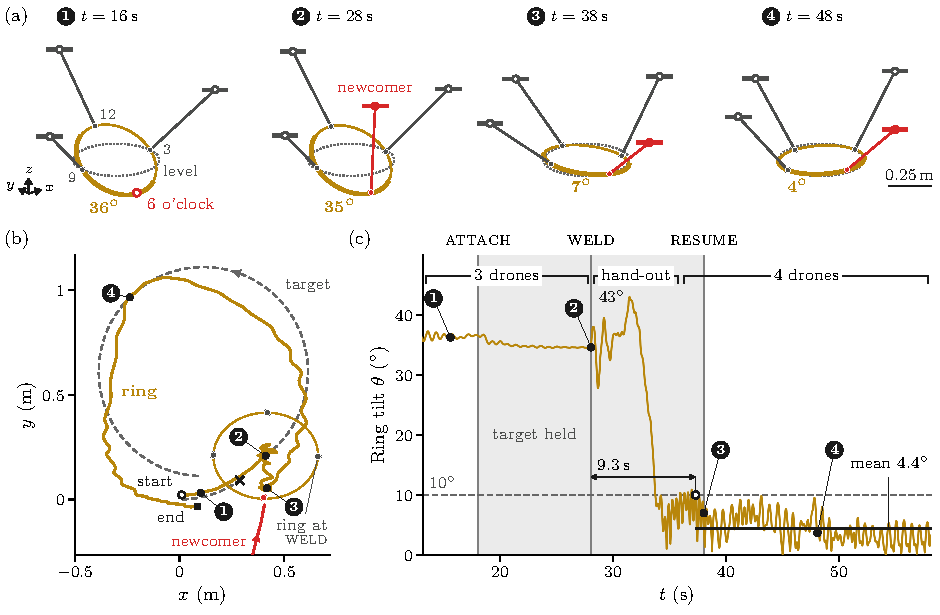
\includegraphics[width=\textwidth]{Images/attach_storyboard.pdf}
% \caption[Attach during a circle]{Attach during a circle in Gazebo (0.6\,kg ring of radius 0.25\,m on 0.5\,m rods). (a) The
% fleet at the four numbered instants, rebuilt from the logged poses in one orthographic view: carriers
% grey, newcomer red; thick: near half of the ring; dotted: the ring if it were level; bar: 0.25\,m.
% (b) Plan view of the ring centre (gold; circle: start, square: end), the payload target (dashed; x:
% held from ATTACH) and the newcomer's approach (red), with the ring and its rim anchors at the weld.
% (c) Ring tilt; grey band: target held; dashed: 10$^\circ$. Three UAVs at 3, 12 and 9 o'clock start
% the circle with the ring tilted by 34--37$^\circ$. ATTACH holds the target and the newcomer welds to
% the empty 6 o'clock rim. During the 8\,s hand-out the tilt first rises to 43$^\circ$; from 9.3\,s
% after the weld it stays under 10$^\circ$ (mean 4.4$^\circ$, peak 9.96$^\circ$), and the four UAVs fly
% the rest of the circle, 0.20\,m RMS from the target against 0.02\,m with three.}
% \label{fig:attach}
% \end{figure}

\redo{the network attach by layout, 3/12/9 o'clock against 4/12/8 o'clock with the newcomer at 6: three-UAV hover tilt, weld transient and four-UAV circle tilt, and the load share of the UAV at 12 o'clock.}
% --- original text, flown before the rig twin; kept to refill this place:
% The sequence completed in every repeat, but it exposed two limits. First, three UAVs on a ring hang it
% tilted when their attachment points leave the centre of mass on the edge of their support triangle:
% at 3/12/9 o'clock the ring hung 27--37$^\circ$ before the weld. The fourth UAV is what levels it.
% Second, the layout trades a level hover against a level circle (Table~\ref{tab:attach_layout}). At
% 3/12/9 o'clock plus 6 the hover is tilted and the four-UAV circle is level. At 4/12/8 o'clock plus 6
% the hover is level, but the UAV at 12 o'clock carries about 40\,\% of the load against 20\,\% for the
% others, and the four-UAV circle rolled by 20--37$^\circ$. A tracker without an integrator sags in
% proportion to its force error, so the most heavily loaded UAV sags most, and a common-mode trim cannot
% correct a differential sag.
%
% \begin{table}[h]
% \centering
% \caption{Network attach on the 0.6\,kg ring by layout (Gazebo).}
% \label{tab:attach_layout}
% \small
% \begin{tabularx}{\textwidth}{>{\raggedright\arraybackslash}Xccc}
% \toprule
% Layout & Three-UAV hover tilt & Weld transient & Four-UAV circle tilt \\
% \midrule
% 3/12/9 o'clock, newcomer at 6 & 33$^\circ$ & 47$^\circ$ peak, 12\,s to settle & 3.7$^\circ$ mean \\
% 4/12/8 o'clock, newcomer at 6 & 2.0$^\circ$ & 10$^\circ$ mean over 4\,s & 20--37$^\circ$ roll \\
% \bottomrule
% \end{tabularx}
% \end{table}

\paragraph{The weld itself.}
\redo{the joint ladder at the weld (ball joint, rod with its inertia, rod with a mid-span joint, rigid weld): flight time after the weld and payload tilt 2\,s and 8\,s after it.}
% --- original text, flown before the rig twin; kept to refill this place:
% \paragraph{The weld itself.} An early hypothesis was that the weld transient came from the
% compliance of the joint between rod and ring. Table~\ref{tab:weld} shows the joint ladder flown to test
% it. A ball joint, a rod with its real inertia and a rod with an extra mid-span joint all behaved alike,
% and a rigid, moment-transmitting weld capsized the payload within 2\,s in five runs out of five.
% Compliance was therefore not the cause. The transient came from the incumbents' tensions stepping to
% their new solution in one tick at the weld, which was then replaced by a blend over the hand-out. The
% attachment is modelled as a ball joint from then on.
%
% \begin{table}[h]
% \centering
% \caption{Payload tilt after the weld by joint model (Gazebo, early attach).}
% \label{tab:weld}
% \small
% \begin{tabularx}{\textwidth}{>{\raggedright\arraybackslash}Xccc}
% \toprule
% Joint at the weld & Flight after the weld (s) & Tilt at +2\,s & Tilt at +8\,s \\
% \midrule
% Ball & 10.1--10.2 & 46--49$^\circ$ & 31--34$^\circ$ \\
% Rod with inertia & 10.4 & 47$^\circ$ & 36$^\circ$ \\
% Rod with mid-span joint & 10.0--10.3 & 40--44$^\circ$ & 26--35$^\circ$ \\
% Rigid & 1.7--1.9 (5 of 5 capsized) & 83--106$^\circ$ & -- \\
% \bottomrule
% \end{tabularx}
% \end{table}

\subsubsection{Attach by OCP resize}

\redo{network attach against attach by OCP resize at the same weld, in hover and in the middle of a circle, on a plant that matches the controller's model (the software-in-the-loop bench, once it flies the twin): payload tilt after the weld.}
% --- original text, flown before the rig twin; kept to refill this place:
% On the 0.86\,kg ring the network attach capsized the payload within about 8\,s of every weld in the
% software-in-the-loop bench, while the OCP resize held the same weld at a peak of about 10$^\circ$, in
% hover and in the middle of a circle. The attach was therefore moved to the OCP resize.

\redo{the attach by OCP resize in Gazebo: the full sequence (approach, weld, resize, resume) in hover; a rejoin during the circle, two runs (weld peak, tilt with four UAVs on the circle, landing); the newcomer's rod pivot below its centre of mass, which the twin has on every UAV; the newcomer's reference aimed along the line to the incumbents' cable apex.}
% --- original text, flown before the rig twin; kept to refill this place:
% In Gazebo the newcomer then flipped 2--5\,s after the weld in every run. The cause was a lever the
% model did not have: the newcomer's arm pivoted 5\,cm below its centre of mass, so the rod's pull,
% modelled at the centre, produced a moment the newcomer's rate loop could not hold. With the pivot at
% the centre, as on the other UAVs, the full sequence (approach, weld, resize, resume) ran clean, with a
% weld peak of 11.6$^\circ$ settling to 0.8$^\circ$. A rejoin during the circle then completed in two
% runs out of two: weld peaks of 10.3--10.5$^\circ$, 0.8--0.9$^\circ$ with four UAVs on the circle, and
% a clean landing. A further correction made the newcomer take its balanced share of the load, aiming
% its reference along the line to the incumbents' cable apex; the weld peaks were then
% 10.7--11.9$^\circ$.

\subsubsection{The rejoin mission}

\redo{the rejoin mission with the collaborator's mission planner: four UAVs on plates 1/3/5/9 on the orbit (radius 0.5\,m at 0.125\,m/s), the UAV on plate~3 detaches, picks up and drops an object into the ring, is handed back, welds onto plate~3 and is folded in, and the fleet lands. Two runs: peak tilt at the detach and at the rejoin, mean tilt over the orbit, height dip at the rejoin, time from TAKEOFF to landed. The fixes found on the way (newcomer tension from 0.1\,N, target shifted onto the measured payload, weld gate on simulation time, damped universal joints on the newcomer's rod, height integral through the orbit) are restated from those runs.}
% --- original text, flown before the rig twin; kept to refill this place:
% The rejoin mission of Section~\ref{sec:reconfig} brings the pieces together with the collaborator's
% mission planner. Four UAVs carry the ring around the orbit (plates 1/3/5/9, radius 0.5\,m at
% 0.125\,m/s). The UAV on plate~3 detaches, flies the collaborator's pick-up and drop of an object into
% the ring, is handed back, welds onto plate~3 and is folded in, and the fleet lands.
% Table~\ref{tab:m1} compares the first complete run with two runs after the fixes listed below.
%
% \begin{table}[h]
% \centering
% \caption{Rejoin mission in Gazebo: first complete run against two runs after the fixes.}
% \label{tab:m1}
% \begin{tabular}{lccc}
% \toprule
%  & First run & After the fixes, run 1 & After the fixes, run 2 \\
% \midrule
% peak tilt at the detach & 5.4$^\circ$ & 2.8$^\circ$ & 2.8$^\circ$ \\
% mean tilt over the orbit & -- & 0.62$^\circ$ & 0.83$^\circ$ \\
% peak tilt at the rejoin & 10.4$^\circ$ & 1.7$^\circ$ & 1.6$^\circ$ \\
% height dip at the rejoin & 6.4\,cm & 1.7\,cm & 1.8\,cm \\
% tilt above 2$^\circ$ after the weld & yes & never & never \\
% TAKEOFF to landed & 115\,s & 115\,s & 133\,s \\
% \bottomrule
% \end{tabular}
% \end{table}
%
% The fixes between the first run and the final pair, each found from a run:
% \begin{itemize}
%     \item the newcomer's tension starts at 0.1\,N instead of 1\,N, and all tensions blend to the
%     balanced solution, which removed the weld moment;
%     \item the target shifts onto the measured payload at the hand-back, since the payload had coasted
%     0.13\,m from its frozen reference by the time of the weld;
%     \item the weld speed gate measures speed over simulation time, not wall time, which had let it weld
%     during the descent;
%     \item the newcomer's rod has damped universal joints at both ends, because the simulator ignores
%     damping on ball joints and the rod's spin was copied onto the ring at the weld;
%     \item the height integral keeps running through a slow, level orbit, which had held the payload
%     6.6\,cm high through the mission.
% \end{itemize}

\redo{the harder rejoin: the payload keeps moving during the rejoin and the newcomer drops a 0.1\,kg object into the ring, two runs (tilt at the detach and at the rejoin, height recovery after the drop, duration).}
% --- original text, flown before the rig twin; kept to refill this place:
% A harder variant has the payload keep moving during the rejoin and the newcomer drop a 0.1\,kg object
% into the ring. Over two runs the detach peaked at 2.6--2.8$^\circ$, the ring was back within 3\,cm of
% its height 4.6--4.7\,s after the drop (lowest 0.491--0.494\,m against 0.60\,m), the rejoin peaked at
% 2.5--3.2$^\circ$ with a 1.1--2.0\,cm dip, and TAKEOFF to landed took 104--133\,s. The spread in
% duration comes from retries inside the collaborator's mission.

\subsubsection{Ground join and hand-over}

\redo{the ground join: the collaborator's controller joins four UAVs to the ring on the floor one at a time and hands them to this work's planner, which lifts, hovers and lands (joins completed, ring height, ring and UAV tilt); with it the hand-over bench under CPU load, body rates from the simulated gyro against differenced poses.}
% --- original text, flown before the rig twin; kept to refill this place:
% In the second integrated case the collaborator's controller joins four UAVs to the ring on the floor,
% one at a time, and hands them over to this work's planner, which sweeps the rods up, lifts the ring to
% 0.60\,m, hovers and lands. Two runs met every target: four joins out of four, the ring at
% 0.600--0.601\,m, peak ring tilt 1.6--1.8$^\circ$ at the lift, 0.6--0.8$^\circ$ in the hover and
% 1.2--2.4$^\circ$ during the descent, and UAV tilt of at most 15.4$^\circ$. The result did not hold when four of the
% next five runs rocked the ring by 7--21$^\circ$. The cause was again the simulator: the collaborator's
% flight controller emulator estimated body rates by differencing unstamped poses, so bunched samples
% under CPU load became rate spikes. On a hand-over bench with the rates taken from the simulated gyro,
% none of six runs under load exceeded 3$^\circ$, against three of six with differenced poses. The full
% ground join on the gyro had no sustained rocking, but both runs had transients of 3.3--3.4$^\circ$
% lasting under half a second, above the 3$^\circ$ bar.


% sim_architecture.tex -- Results: trajectory-based planner against the dissipative network
% (draft 4 Oct 2026). Sources: docs/design/velocity_loop.md sections 1, 8-11 (Part A study, Aug 2026,
% early 0.4 kg payload, n=3 circle r 0.5 at 0.6 m/s, medians over 5 and 3 runs, R0054-R0077);
% CURRENT_STATE 4.4 (INDI table: R0234, R0244, R0247, R0255, R0257), 6 (negatives).

\subsection{Trajectory-based planner against the dissipative network}
\label{sec:sim_architecture}

The two approaches are compared on the same plant and the same trackers, in carrying, detach and
attach. This addresses RQ2.

\paragraph{Where the network's tracking error comes from.}
\redo{the network flying a circle with the MPC tracker (three UAVs, radius 0.5\,m): the payload's radius ratio and lag, split by stage (desired path to the network's references, references to UAVs, UAVs to payload).}
% --- original text, flown before the rig twin; kept to refill this place:
% \paragraph{Where the network's tracking error comes from.} With the network flying a circle (three
% UAVs, radius 0.5\,m at 0.6\,m/s, early payload), the payload traced a circle 18\,\% too small and
% 0.68\,s late. Splitting the chain into stages located the error. From the desired path to the
% centroid of the network's references the radius ratio was 0.94 with a lag of 0.30\,s. From the
% references to the UAVs it was 0.87 and 0.54\,s, and from the UAVs to the payload 1.00 and $-0.12$\,s.
% The largest loss was in the tracker: a stiff position MPC with a 2\,s horizon, a stage that the
% architecture of \cite{quan2025swarm} does not have, since its robots take velocity commands.

\paragraph{Velocity tracking.}
\redo{the tracking architecture under the network on the same circle, medians over repeats: MPC tracker, velocity loop, velocity loop with the common-mode trim (radius ratio, phase lag, payload RMSE, payload height, tilt after the sweep); and an integrator in each UAV's velocity loop.}
% --- original text, flown before the rig twin; kept to refill this place:
% \paragraph{Velocity tracking.} The velocity loop of Section~\ref{sec:dissipative} removes that
% stage. Table~\ref{tab:arch} shows the effect. The radius ratio went from 0.82 to 1.00, the lag fell
% by a quarter, and the payload error over the sweep fell from 0.27 to 0.22\,m. The cost was payload
% tilt after the manoeuvre, 5.4$^\circ$ against 1.4$^\circ$. An integrator in each UAV's velocity loop
% tilted the payload to 60$^\circ$, because the UAVs integrate different errors and the differences
% become a moment. The common-mode trim, one integrator for the whole team, brought the payload to its
% target height without changing the tracking.
%
% \begin{table}[h]
% \centering
% \caption{Tracking architecture with the dissipative network, circle of radius 0.5\,m at 0.6\,m/s,
% three UAVs, early payload (median over 3--5 runs).}
% \label{tab:arch}
% \begin{tabularx}{\textwidth}{Xccc}
% \toprule
%  & MPC tracker & Velocity loop & + common-mode trim \\
% \midrule
% payload radius ratio & 0.816 & 1.001 & 1.001 \\
% payload phase lag (s) & 0.676 & 0.514 & 0.514 \\
% payload RMSE over the sweep (m) & 0.272 & 0.215 & 0.215 \\
% payload height (m), target 0.60 & 0.498 & 0.498 & 0.600 \\
% payload tilt after the sweep & 1.4$^\circ$ & 5.4$^\circ$ & 5.4$^\circ$ \\
% \bottomrule
% \end{tabularx}
% \end{table}

\paragraph{Reconfiguration.}
\redo{no flights of its own: the trajectory-based planner against the network on a detach and on an attach, restated from the comparisons of Sections~\ref{sec:sim_detach} and~\ref{sec:sim_attach} once those are re-flown.}
% --- original text, flown before the rig twin; kept to refill this place:
% \paragraph{Reconfiguration.} In both reconfiguration directions the trajectory-based planner did
% better. On a detach, the OCP resize held the payload level where the network hand-off left it tilted
% by 26--48$^\circ$ (Section~\ref{sec:sim_detach}), and on the 0.86\,kg ring the network aborted at
% 53--61$^\circ$. On an attach, the network capsized the 0.86\,kg ring within about 8\,s of the weld
% while the OCP resize held it at about 10$^\circ$ (Section~\ref{sec:sim_attach}).

\paragraph{Stiff trackers and slack rods.}
\redo{the measured-force throttle on the network attach during a circle: model-based (MPC), measured force at gain 1, at gain 0.5, and at gain 0.5 with an anti-swing term (tilt 4--10\,s after the weld, circle tilt, outcome).}
% --- original text, flown before the rig twin; kept to refill this place:
% \paragraph{Stiff trackers and slack rods.} A measured-force throttle (the thrust command corrected by
% the measured acceleration, after the incremental nonlinear dynamic inversion \cite{smeur2016indi} used by
% \cite{tudelft}) made each
% UAV exact at its own position. On the network attach it was worse, not better
% (Table~\ref{tab:indi}). At full gain the payload tilt grew at about 1\,Hz until the flight aborted.
% A UAV that holds its position exactly turns the payload into a load hanging from fixed points on
% rods whose lengths the network only approximates. Rods then go slack, and a payload on
% intermittently slack rods swings. The compliant MPC tracker kept the rods taut by sagging into the
% load. Half gain with an anti-swing term was the best compromise, and the throttle was removed.
%
% \begin{table}[h]
% \centering
% \caption{Measured-force throttle on the network attach during a circle (0.6\,kg ring, Gazebo).}
% \label{tab:indi}
% \small
% \begin{tabularx}{\textwidth}{>{\raggedright\arraybackslash}Xcc>{\raggedright\arraybackslash}X}
% \toprule
% Throttle & Tilt 4--10\,s after weld & Circle tilt, mean / max & Outcome \\
% \midrule
% Model-based (MPC) & 28.8$^\circ$ & 3.7 / 9.4$^\circ$ & completes \\
% Measured force, gain 1 & 7.1$^\circ$ & -- & 1\,Hz tilt growth, abort \\
% Measured force, gain 0.5 & 17.4$^\circ$ & 8.5 / 16$^\circ$ & completes \\
% Gain 0.5 + anti-swing & 18.2$^\circ$ & 5.7 / 11.1$^\circ$ & completes \\
% \bottomrule
% \end{tabularx}
% \end{table}

\paragraph{Closing the loop on the payload's pose.}
\redo{the network variants that use the payload's measured state: tensions solved at the measured attitude, a horizontal leash to the measured position, the cone tilted onto the effective gravity, and an admittance on the measured rod tension, each against the open-loop network.}
% --- original text, flown before the rig twin; kept to refill this place:
% \paragraph{Closing the loop on the payload's pose.} Several variants tried to give the network
% feedback from the payload's measured state, and each made it worse:
% \begin{itemize}
%     \item solving the tensions at the payload's measured attitude raised the weld transient to
%     68$^\circ$ and aborted both runs;
%     \item a horizontal leash towards the payload's measured position closed a position loop, after
%     which the flight aborted and the newcomer never welded;
%     \item tilting the cone onto the effective gravity gave no radius benefit and contracted the
%     formation further;
%     \item an admittance on the measured rod tension was biased by the thrust model and made the
%     hover worse.
% \end{itemize}
% The network is therefore kept open-loop in the payload's pose, apart from the common-mode height
% trim.

\paragraph{Summary.}
\redo{no flights of its own: the verdict of this comparison (tracking, detach, attach), rewritten from the re-flown results above.}
% --- original text, flown before the rig twin; kept to refill this place:
% \paragraph{Summary.} On this system, with rigid rods, a heavy ring and Betaflight UAVs, the
% trajectory-based planner was better in tracking, in detach and in attach. The network's strengths in
% \cite{quan2025swarm}, namely no solver per team size and passive tolerance of a member leaving, did
% not carry over. Its dissipation acts on virtual nodes rather than on the payload, its geometry
% cannot use the payload's measured pose without destabilising it, and it relies on a cable feedforward
% that matches the real rod force, which a tracker without an integrator turns directly into a sag or
% a tilt. The OCP resize needs one pre-built solver per team size, which for two to four UAVs is cheap.


% sim_robustness.tex -- Results: robustness to wrong parameters (draft 4 Oct 2026).
% Sources: CURRENT_STATE 4.7 (E10, R0215-R0222, 10 Sep, attach demo, 0.6 kg ring), 4.8 (measure_rod_len,
% SIL R0308-R0327, 23 Sep, quadratic plant, notes 2026-09-23_geometry_autocal), 4.10 (kt_trim,
% R0405-R0432, notes 2026-09-23_kt_trim), decisions 2026-09-25 (height integral: R0557 0.661 vs
% R0558 0.600; pair 0.658 x2 vs 0.600 x3).
% All of these were flown with the tracker's node-0 box at 0.025 (default until 4 Oct), which is the
% +3.4 cm of the 0.634 baselines; the differences between arms are the result.
% T9 (tab:robust): R1038-R1067 (5 Oct, box 0, land fix), no-error baseline z_ki 0 R1013/R1023;
% generator tools/thesis_sim_tables.py table_robust.

\subsection{Robustness to wrong parameters}
\label{sec:sim_robustness}

The controller is given the payload's mass, the rod lengths and the attachment radius, and each UAV's
thrust map. On the rig each of these is measured, and each can be wrong. This subsection collects the
tests of what a wrong value does.

\paragraph{The current controller.} Table~\ref{tab:robust} gives the rig twin's hover at 1.0\,m, three
UAVs from a floor start, with one wrong value in the controller while the simulated rig keeps the true
ones. Each case was flown without and with the height integral.
\begin{itemize}
    \item A wrong payload mass moves the hover by about 1.25\,cm per percent of mass, the same in
    both directions. The integral removes it while the miss is inside its 0.25\,m gate, with a target
    shift that mirrors the error. A 20\,\% overestimate puts the ring 2\,mm over the gate, so the
    integral never starts and the ring holds 26\,cm high: a miss beyond the gate is not taken for a
    static offset. The bound matters as well: the 20\,\% underestimate needs 23\,cm of shift, which
    the earlier bound of 0.15\,m would have cut off, and the planner warns that the integral is near
    its bound.
    \item Measuring the rods at the hand-over absorbs a 5\,cm rod error completely. Without the
    measurement the ring sits 8\,cm high, and the integral does not help: a rod typed 5\,cm long
    measures as only partly taut, and the integral waits for every rod to be taut. For rods typed
    long, the measurement is therefore what makes the integral available; a rod typed short reads as
    taut, and that case was not flown.
    \item A 2\,cm error in the attachment radius has no visible effect.
\end{itemize}
The ring's tilt stayed within 1.0--1.3$^\circ$, slightly lower with the mass typed high, and all 28
flights landed.

\begin{table}[htbp]
\centering
\caption[Hover with a wrong model]{Hover at 1.0\,m with one wrong value in the controller's model,
Gazebo rig twin, three UAVs, $\epsilon = 0$, floor start. Each cell is the mean of two runs. Target
shift: the integral's correction to the height target at LAND. Tilt: mean over the four runs.
Landed: flights that landed without a tip. $^a$~The miss is over the integral's 0.25\,m gate, so the
integral never starts. $^b$~The unmeasured rods read as partly slack, so the integral's tautness
gate stays closed.}
\label{tab:robust}
% generated by tools/thesis_sim_tables.py
\begin{tabularx}{\textwidth}{>{\raggedright\arraybackslash}Xccccc}
\toprule
 & \multicolumn{2}{c}{Height error (cm)} & Target & & \\
\cmidrule(lr){2-3}
Error in the controller's model & no integral & integral & shift (cm) & Tilt (\si{\degree}) & Landed \\
\midrule
none & $+$0.9 & 0.0 & $-$0.8 & 1.2 & 4/4 \\
payload mass typed $+10$\,\% & $+$13.5 & 0.0 & $-$13.4 & 1.1 & 4/4 \\
payload mass typed $+20$\,\% & $+$25.8 & $+$25.8$^a$ & 0.0 & 1.0 & 4/4 \\
payload mass typed $-20$\,\% & $-$23.5 & 0.0 & $+$23.3 & 1.3 & 4/4 \\
rods typed $+5$\,cm, measured at the hand-over & $+$0.9 & $+$0.1 & $-$0.9 & 1.2 & 4/4 \\
rods typed $+5$\,cm, not measured & $+$8.2 & $+$8.2$^b$ & 0.0 & 1.1 & 4/4 \\
attachment radius typed $+2$\,cm & $+$0.9 & 0.0 & $-$0.9 & 1.2 & 4/4 \\
\bottomrule
\end{tabularx}

\end{table}

\paragraph{Rod length and attachment radius.}
\redo{hover with a wrong typed geometry, with and without the rod measurement at the hand-over, for the cases Table~\ref{tab:robust} does not have: rods typed short, the attachment radius typed 2\,cm short, and the combination (rods and radius wrong with the payload mass typed 20\,\% low).}
% --- original text, flown before the rig twin; kept to refill this place:
% \paragraph{Rod length and attachment radius.} The tautness gate scales each UAV's cable feedforward
% by its measured rod length over the typed one. A rod 4\,cm shorter than typed therefore reads as
% partly slack, the fleet flies about half of the cable feedforward, and the payload hangs 22\,cm low.
% Measuring the rods at the hand-over (Section~\ref{sec:takeoff}) removes this
% (Table~\ref{tab:rodlen}): rod errors of $\pm 4$\,cm and attachment-radius errors of $\pm 2$\,cm are
% absorbed to within 1\,cm, and with no error the measurement changes nothing. A mass error is not
% addressed by the measurement; with the payload 20\,\% heavier than typed the hover sat 9\,cm lower.
%
% \begin{table}[h]
% \centering
% \caption{Hover height with a wrong typed geometry, with and without measuring the rods
% (software-in-the-loop, target 0.60\,m, two runs each agreeing to 1\,mm).}
% \label{tab:rodlen}
% \begin{tabularx}{\textwidth}{>{\raggedright\arraybackslash}Xccc}
% \toprule
% Error & Measurement off & Measurement on & Measured rod \\
% \midrule
% none & 0.634 & 0.634 & 0.500 \\
% rod 0.46\,m, typed 0.50\,m & 0.416 & 0.631 & 0.460 \\
% rod 0.50\,m, typed 0.46\,m & 0.569 & 0.634 & 0.500 \\
% radius 0.27\,m, typed 0.25\,m & -- & 0.642 & 0.514 \\
% radius 0.23\,m, typed 0.25\,m & -- & 0.626 & 0.486 \\
% payload mass +20\,\% & -- & 0.540 & 0.500 \\
% rod $-4$\,cm, radius $-2$\,cm, mass +20\,\% & -- & 0.549 & 0.474 \\
% \bottomrule
% \end{tabularx}
% \end{table}

\paragraph{Mass and rod length during an attach.}
\redo{a wrong payload mass ($\pm 25$\,\%) or rod length ($\pm 10$\,\%) in the controller during an attach, two runs each: whether the flight completes, and the payload height after the weld.}
% --- original text, flown before the rig twin; kept to refill this place:
% \paragraph{Mass and rod length during an attach.} On the attach demonstration the controller was told
% a wrong mass or rod length while the simulated plant kept the true ones (two runs each). Telling it
% the payload is 25\,\% lighter, or the rods 10\,\% shorter, than they are was absorbed: both runs
% completed. Telling it the payload is 25\,\% heavier over-lifted the payload to 0.96\,m, and telling it
% the rods are 10\,\% longer dropped it to 0.17\,m; both aborted within about 10\,s of the weld. The
% envelope is asymmetric. An underestimate is made up by the height trim, while an overestimate plans
% more pull than the payload needs. On the rig the payload is weighed and the rods measured, and a
% doubtful value is entered low.

% CUT 5 Oct 2026 (legacy-only, not to be redone): the thrust-gain trim (kt_trim), a legacy-plant feature that is off on the rig and the twin.
% \paragraph{Thrust map.} A per-UAV estimate of the throttle-to-acceleration gain, computed from the
% UAV's own measured acceleration and its static share of the cable force, was built to correct a
% typed gain that is wrong. In the software-in-the-loop bench it brought the hover from 0.499 and
% 0.461\,m back to 0.614\,m with the gain typed 10 and 15\,\% high, with the estimates converging to
% within 1\,\% of the true gain, 3--9\,s after TAKEOFF and without overshoot. In Gazebo, from a floor start with the
% gain typed 10\,\% high, the fleet parked at 0.53\,m without it and lifted to 0.609\,m with it. It needed
% a floor-contact test, because while a UAV rests on the floor the floor carries part of its weight
% and the estimate read that as strong motors. With two UAVs it chattered at 2\,Hz until its inputs were
% time-aligned. On the rig the thrust map was instead identified directly (Section~\ref{sec:hardware}),
% and the estimate is kept off.

% CUT 5 Oct 2026 (legacy-only, not to be redone): the first height-integral test, superseded by Table tab:robust and the disturbance table.
% \paragraph{Height integral.} The bounded height integral on the target (Section~\ref{sec:disturbance})
% was first tested on a hover that sat high without it: 0.658\,m in two runs without the integral
% against 0.600\,m in three runs with it. In software-in-the-loop it held 0.600\,m in every static-offset
% case in both directions, stayed inert through the circle, and saturated with a warning when the error
% was a large gain fault rather than an offset.


% rig_results.tex -- Results: hardware (draft 4 Oct 2026). No run ids in the text.
% Sources: docs/rig_2026-09-30_review.md, rig_2026-09-30_replay.md, rig_2026-09-30_force_balance.md,
% registry RIG-0930-* and RIG-1001-* (h1, h2-z080, c1-z100, f8-z100, h5-z100-rot120, h6-z100-xp60),
% logs results/rig/2026-10-01/<flight>_logs; B4 offline replay (2026-10-01_load_ext_force.md);
% CURRENT_STATE 7 items 8 and 10 (16 and 23 Sep); twin R0817/R0818, R0834-R0839.
% The H6 drift is 2.8 cm in the registry and 4.5 cm in the 3 Oct review recompute: reported as 3-5.
% FIGURE TODO (thesis-figure skill): 1 Oct ring height vs time for H1/H2/C1/H5 with the cap and the
% integral; tilt vs ring height; plan view of the -x drift with the rotation test.

\subsection{Hardware results}
\label{sec:rig_results}

The hardware campaign so far covers carrying the ring with three and four UAVs. Neither detach nor
attach has been flown on the rig. The rig is available about two days a week, and each day
followed the simulation work of the days before it, so each is summarised with what it showed and
what changed as a result.

\subsubsection{Rig days}

\begin{table}[h]
\centering
\small
\caption{Rig sessions with the payload.}
\label{tab:rig_days}
\begin{tabularx}{\textwidth}{lX}
\toprule
Date & What was flown and what it showed \\
\midrule
3 Aug & First flights of the planner stack on the rig. Fixed: attachment slots matched in the
payload's frame (a yawed payload made the problem infeasible), a latched payload yaw datum, a latched
heading per UAV (one UAV turned a full circle on takeoff), trackers on the correct clock. \\
16 Sep & First carry attempts with the planner from the floor: the payload did not lift. One UAV per
flight spun in yaw at spool-up, later traced to the tracker's yaw command on a tilted floor rest. The planner's references assumed taut rods and sat inside
the UAVs (Section~\ref{sec:takeoff}). \\
23 Sep & Two UAVs, rods typed 0.50\,m against a real 0.46\,m, thrust gain typed: the payload did not
leave the floor and the UAVs drifted in over it. One battery sagged from 21.2 to 17\,V. Found: battery
thresholds set for a smaller battery, and the need for the rod sweep. \\
30 Sep & Four UAVs, 0.86\,kg ring. First lifts and the first sustained carry (12.6\,s at 0.28\,m). Seven
bugs fixed on the day. The thrust map identified (Section~\ref{sec:hardware}). Breakaway at 60--80\,\%
of the planned pull. Last flight: ring held 16\,cm low with a 14\,cm heave at 0.17\,Hz, and 25 planner
solve failures. \\
1 Oct & Three UAVs (one airframe out of service), six flights to 1.0\,m including a circle and a
figure-eight, with no solve failures (Table~\ref{tab:rig_oct1}). \\
\bottomrule
\end{tabularx}
\end{table}

\paragraph{30 September.} The day went from a ring that would not leave the floor to sustained
carries. The bugs found on the day each had a clear signature in the logs. The creep fed the UAVs to the
wrong plates, so the fleet flew into the middle of the ring. The cable feedforward was zeroed while the
ring rested, so the lift deadlocked. Only one UAV received the pull flag. The pull arrived as a step
and launched the ring, releasing two magnets. Each was fixed and then flown, which is how the
pretension and breakaway procedure of Section~\ref{sec:takeoff} came about. Two problems remained at
the end of the day: the ring was held low, and the planner failed to solve 25 times in the last
flight. A replay of the planner on the logged states traced the failures to two faults acting
together. The UAVs sat 30$^\circ$ round from the attachment points the planner modelled, one plate off,
and the payload's measured quaternion changed sign when its yaw crossed 180$^\circ$. Removing either
removed every failure in the replay. The planner now keeps the quaternion's sign continuous and
warns before ARM if a UAV sits more than 10$^\circ$ from its slot. None of the 1 October flights had a
solve failure.

\paragraph{Thrust identification.} Each UAV hovered free with masses of 0, 98 and 196\,g hung from it,
on batteries between 22.7 and 24.6\,V. The 13 points fit the affine map of
Section~\ref{sec:hardware}, $u_T = a_i + 0.507 M - 0.022 (V - 23.5)$, with offsets $a_i$ of 0.181 to
0.187 and a residual of 0.003 rms. With the map and one shared offset, the four UAVs hovered free at
+3.7, $-0.5$, $-0.4$ and +0.9\,cm from their targets with no integral action. In tethered flight the
throttle the UAVs needed (0.55--0.60) matched what the map predicted for their share of the load
(0.569--0.575).

\subsubsection{1 October: three UAVs to 1.0\,m}

\begin{table}[h]
\centering
\small
\caption{Rig flights on 1 October, three UAVs on plates 0/4/8. Breakaway: fraction of the planned
pull at which the ring left the floor; it was held for the whole flight. Height integral bound
0.15\,m. Tilt and the horizontal offset are over the hold; $^{\dagger}$ marks the mean distance from
the trajectory reference over the manoeuvre. Orbit: radius 0.5\,m at 0.125\,m/s; figure-eight:
$a = 0.5$\,m at 0.2\,m/s. Rotated: the whole system turned by 124$^\circ$; moved: shifted 1.1\,m
towards $+x$.}
\label{tab:rig_oct1}
\footnotesize
\begin{tabularx}{\textwidth}{>{\raggedright\arraybackslash}Xcccccc}
\toprule
Flight & Target & Held & Integral & Tilt & Offset & Break- \\
 & (m) & (m) & & mean / max & (cm) & away \\
\midrule
Hover & 0.5 & 0.45 & off & 5.0 / 13.8$^\circ$ & 5.7 & 80\,\% \\
Hover & 0.8 & 0.67 & at bound & 2.5 / 6.7$^\circ$ & 11.8 & 73\,\% \\
Orbit & 1.0 & 0.94 & at bound & 1.6 / 4.1$^\circ$ & 15.1$^{\dagger}$ & 83\,\% \\
Figure-eight & 1.0 & 0.67 & never on & 3.2 / 9.0$^\circ$ & 18.8$^{\dagger}$ & 73\,\% \\
Hover, rotated & 1.0 & 1.01 & at bound & 3.8 / 6.6$^\circ$ & 8.1 & 93\,\% \\
Hover, moved & 1.0 & 0.89 & at bound & 2.2 / 4.1$^\circ$ & 3--5 & 77\,\% \\
\bottomrule
\end{tabularx}
\end{table}

All six flights lifted cleanly. The rod sweep handed over at 51--55$^\circ$, as in the twin, and the
measured rods read 0.531--0.556\,m against 0.55\,m typed. The orbit completed a full lap and the
figure-eight its whole path, and every flight landed. Three results stand out.

\paragraph{The ring sat low.} Without the height integral the ring held 5\,cm low at 0.5\,m, and at
higher targets it sat 20--30\,cm low before the integral took over, which then saturated at its bound.
The figure-eight, where the integral does not run, held the ring 29\,cm low. The shortfall was largest
on the flights whose ring broke free at the smallest fraction of the planned pull. The cause was
found afterwards in the logs: the breakaway freeze had held the pull at that fraction for the whole
flight, so the trackers were told the rods pull 7--27\,\% less than they do. Holding the pull at
75\,\% in the Gazebo twin reproduced both symptoms on the rig: the ring 23--26\,cm low and the rods
steepened from 52 to 58$^\circ$. Releasing the cap once the lift starts restored the twin's height
to the no-cap value (Section~\ref{sec:sim_to_real}). This fix has not yet been flown.

\paragraph{Tilt fell with height.} Over the first three flights the ring's mean tilt fell from
5.0$^\circ$ at 0.45\,m to 2.5$^\circ$ at 0.67\,m and 1.6$^\circ$ at 0.94\,m; the later hovers at
0.9--1.0\,m had 2.2--3.8$^\circ$. Close to the floor the ring sits in the UAVs' downwash and its
recirculation off the floor, and flying higher was the most effective single change for a steady
ring.

\paragraph{The ring drifted towards $-x$.} In every flight the ring sat 3--17\,cm from its horizontal
reference, always towards the room's $-x$ direction, and nothing in the controller pulled it back.
The offset kept its direction when the whole system (ring and UAVs) was rotated by 124$^\circ$, so it
does not come from a particular UAV, rod or the ring. The force behind it was estimated offline from
the logs: the UAVs' delivered thrust, from the identified map and their measured attitudes, less the
total weight. Over the steady holds this gives a horizontal force of 0.41--0.52\,N towards $-x$,
about 1$^\circ$ of the fleet's thrust. At the planner's horizontal stiffness of about 5\,N/m that
explains offsets of 8--10\,cm. Moving the system 1.1\,m towards $+x$ reduced the offset to 3--5\,cm,
in a single flight. Two explanations remain open: a ground plane in the motion-capture calibration
tilted by about 1$^\circ$, which would put a component of gravity along $x$ in the frame the
controller works in, or air moving in the room. A plumb-line check of the calibration comes first at
the next session.

\subsubsection{Simulation against the rig}
\label{sec:sim_to_real}

Table~\ref{tab:sim_vs_rig} sets the twin's hover at 1.0\,m against the rig's flights at the same
target. The twin comparison of the breakaway cap was flown with four UAVs and the rig with three, so
the comparison is of mechanisms rather than of exact values. The twin matched the rig in the takeoff
geometry and in solver health, and a single setting, the breakaway cap, accounted for the height
difference. The twin did not show the horizontal drift, the
larger tilt at low height or the slower breakaway.

\begin{table}[h]
\centering
\small
\caption{Hover at 1.0\,m: Gazebo rig twin (four UAVs, before the tracker fix) against the rig on
1 October (three UAVs). The twin with the cap held at 0.75 reproduces the rig's pull.}
\label{tab:sim_vs_rig}
\begin{tabularx}{\textwidth}{>{\raggedright\arraybackslash}Xccc}
\toprule
 & Twin, cap released & Twin, cap held at 0.75 & Rig, 1 October \\
\midrule
hand-over elevation & 55.4--55.7$^\circ$ & 55--56$^\circ$ & 51--55$^\circ$ \\
measured rods (m) & 0.550 & 0.550 & 0.531--0.556 \\
breakaway, fraction of the pull & about 0.97 & 0.75 (set) & 0.73--0.93 \\
ring height before the integral (m) & 1.03 & 0.77 & 0.71--0.81 \\
rod elevation in the hold & 52$^\circ$ & 58$^\circ$ & 57--65$^\circ$ \\
ring tilt, mean & 1.2$^\circ$ & 1.3$^\circ$ & 1.6--3.8$^\circ$ \\
horizontal offset in hover & under 1\,cm & under 1\,cm & 3--17\,cm \\
planner solve failures & 0 & 0 & 0 \\
\bottomrule
\end{tabularx}
\end{table}


% discussion.tex -- Results: discussion (draft 4 Oct 2026). To be revised once the hardware detach,
% the four-UAV rig flights and the rig-twin attach are in.

\subsection{Discussion}
\label{sec:discussion}
% 9 Oct (structure audit): the list of simulator artefacts moved here from the experimental method;
% the steady-error taxonomy points at Table tab:error_sources.

This section answers the questions in order, then discusses what the results mean beyond them: the
role of geometry, the steady errors of a re-planned cascade, the twin against the rig, and the
limitations.

\paragraph{RQ1: a centralised controller through join and leave.} In simulation the answer for the
detach is yes, with a condition. A detach by OCP resize redistributes the load in the first solve after the release,
and the payload settles level within a few seconds, provided the survivors' attachment points still
surround its centre of mass. The centralised planner's advantage is that it knows the
whole attachment geometry. It does not have to discover the new load distribution from the motion
that follows the event: it solves for it. This supports the hypothesis of the project plan. Neither
reconfiguration has been flown on the rig.
% CHECK: stale since the 7-8 Oct rig detach flights (Section 4.3, fig:rig_detach).

\redo{the attach half of RQ1: the weld transient of an attach by OCP resize in the full rejoin mission (Section~\ref{sec:sim_attach}).}
% --- original text, flown before the rig twin; kept to refill this place:
% \paragraph{RQ1: a centralised controller through join and leave.} In simulation the answer is yes,
% with a condition. A detach by OCP resize redistributes the load in the first solve after the release,
% and the payload settles level within a few seconds, provided the survivors' attachment points still
% surround its centre of mass. An attach by OCP resize folds the newcomer in with a weld transient of
% under 2$^\circ$ in the full rejoin mission. The centralised planner's advantage is that it knows the
% whole attachment geometry. It does not have to discover the new load distribution from the motion
% that follows the event: it solves for it. This supports the hypothesis of the project plan. Two parts
% of the answer are not yet in. Neither reconfiguration has been flown on the rig, and the attach
% results come from the earlier simulation geometry, before the rig twin.

\redo{the attach's hand-over faults (mux authority on an armed but idle stream, the newcomer's starting tension, the frozen target, the weld gate's clock), restated once the attach has flown on the twin.}
% --- original text, flown before the rig twin; kept to refill this place:
% The attach needed much more than the resize. Most of the faults that blocked it were in the hand-over
% between two controllers, not in either controller. A multiplexer gave authority to a stream that was
% armed but idle. A newcomer started with too much tension pulled the ring with a lever about the
% incumbents' apex. A frozen target let the payload coast away from the approach. A weld gate measured
% speed in the wrong clock. A joining UAV is a hand-over problem as much as a control problem, and
% each interface needed an explicit rule for who commands the UAV and when.

\paragraph{RQ2: trajectory-based against dissipative.}
\redo{the answer to RQ2 (trajectory-based planner against the dissipative network in tracking, detach and attach), rewritten from the re-flown comparison of Section~\ref{sec:sim_architecture}.}
% --- original text, flown before the rig twin; kept to refill this place:
% \paragraph{RQ2: trajectory-based against dissipative.} On this system the trajectory-based planner was
% better in every test: tracking, detach and attach. The dissipative network did as well as the
% literature suggests only once its tracker was replaced with the velocity loop it assumes, and even then
% it was not robust to a heavier payload. Its strengths are real but did not apply here. With rigid rods
% the payload is held by geometry, which the network can only approximate. Its dissipation acts on
% virtual nodes rather than the payload. And it cannot use the measured payload pose without
% destabilising itself. A combination remains possible, with the planner for tracking and
% reconfiguration and a compliant layer at the weld, but with the OCP resize the evidence does not call
% for it.

\paragraph{Geometry decides what control can do.}
\redo{the geometry cases behind this paragraph: three UAVs at 3, 12 and 9 o'clock hanging the ring tilted, the even ring of four after a detach, the ring on two rim points, and the uneven layout's load share turning into a roll (Sections~\ref{sec:sim_detach} and~\ref{sec:sim_attach}).}
% --- original text, flown before the rig twin; kept to refill this place:
% \paragraph{Geometry decides what control can do.} Several results that first looked like control
% problems were geometry. Three UAVs at 3, 12 and 9 o'clock hang the ring tilted, because its centre of
% mass lies on the edge of their support triangle. An even ring of four loses its support after one
% UAV leaves. A ring on two rim points is a pendulum. An uneven layout puts 40\,\% of the load on one
% UAV, which a tracker without an integrator turns into a roll. Choosing the attachment layout for the
% reconfigurations that will happen is part of the design, and a simple test (is the centre of mass
% inside the support polygon, and by how much) predicts which layouts will work.

\paragraph{Steady errors in a re-planned cascade.} The planner re-solves from the measured state at
every tick, which closes a loop on the payload's position with no integrator. In the twin its
stiffness is about 5\,N/m horizontally and 7\,N/m vertically, so a force of half a newton moves the
payload by 7--10\,cm and stays. The investigation of the payload's height and horizontal offsets
separated four kinds of cause (Table~\ref{tab:error_sources}):
\begin{itemize}
    \item a bias in the cascade itself: the tracker's relaxed initial condition, which held the payload
    about 5\,cm high and which no force estimate could find, because it is not a force;
    \item a wrong belief passed between levels: the breakaway cap, which told the trackers the rods
    pull up to 27\,\% less than they do, and left the rig's ring 20--30\,cm low;
    \item model errors: the rods' mass, one UAV's thrust map;
    \item external forces: a push, wind, and the rig's steady pull towards $-x$.
\end{itemize}
Integral action removes the steady error from all of them, as the internal model principle says, but
only where its gate is open and within its bound. Whether the integral moves the target or acts as a
force in the planner's model changes the transient and what the plan predicts, not the steady state.
A force estimated from motion and thrust removes external forces quickly, but by Newton's law it is
blind to forces the system exerts on itself. A wrong thrust map on one UAV is a moment on the ring,
and only a correction of that UAV's own force removes it. In \cite{tudelft} the onboard incremental
inversion makes each UAV exact at its own force, at 300\,Hz from rotor speed, which is why the planner
needs no integrator there. With Betaflight and a ground-side controller the equivalent was the
measured-cable-force tracker. It levelled the ring against a wrong thrust map, but in this
configuration it upset the landings, so integral action in the planner is the practical substitute.

\paragraph{Simulation and the rig.} The rig twin, flown on exactly the rig's code, matched the rig in
the takeoff (hand-over angle, rod lengths) and in solver health. It also reproduced the rig's height
shortfall from the one setting that caused it. It did not reproduce three things: the slower
breakaway (73--93\,\% of the planned pull against about 97\,\%), the larger tilt near the floor, and
the steady pull towards $-x$. The first is suspected to be an effect near the floor, the second the
downwash, the third the room or its calibration. None of them is modelled. Many apparent controller
faults in simulation turned out to be simulator artefacts, each of which had to be found and removed
before the twin could be trusted:
\begin{itemize}
    \item rate estimates differenced from unstamped poses turned bunched samples into rate spikes under
    CPU load, so the emulated rate loop now uses the gyro;
    \item a proportional-only emulated rate loop could not hold the moment of a rod pivoting below a
    UAV's centre, and flipped UAVs when control was handed over;
    \item the physics engine ignores damping on ball joints, so a damped rod needs universal joints;
    \item wall-clock watchdogs fire when the simulation runs slower than real time, which it does
    (about 0.3 of real time with the full stack on the laptop).
\end{itemize}
Finding them took as long as the controller work.

\paragraph{Limitations.} The work is at lab scale (a 0.86\,kg payload, two to four UAVs, a
6\,$\times$\,6\,m room) with motion capture as the only sensing and all computation on one ground
computer. The rods are rigid, so slack cables are outside the model. The attach depends on an
electromagnet and on a collaborator's approach controller. The hardware results so far cover carrying
only, with three UAVs on 1 October.
% CHECK: stale since the 7-8 Oct rig flights (four UAVs; the detach flown on the rig).
Several simulation tables rest on single runs or on earlier code,
and are marked as such; they will be re-flown on the final code before the results are frozen.


% STILL TO DO (5 Oct 2026):
%   - Everything flown before the rig twin is marked in the text with a \redo box; the list of what
%     to fly for each box (arms, prerequisites, priority) is docs/redo_on_twin.md in the code repository.
%   - Hardware (from 7 Oct): breakaway cap release, four UAVs on 0/3/6/9 and 1/3/5/9, orbit and
%     figure-eight at 1.0 m, the mocap level check, detach 4 -> 3 in hover; later the attach.
%   - Comparisons with the literature: TU Delft (hover and circle tracking error normalised by
%     radius, tilt), Quan (dropout transient, robustness to cable length and mass), Bacheti
%     (re-spacing after a detach).
%   - Figures (thesis-figure skill): rejoin storyboard on the M1 run; detach tilt vs time by
%     layout with the support-polygon plan view; thrust identification (throttle vs mass per UAV,
%     fit and residuals); 1 Oct ring height vs time with the cap and the integral; tilt vs height.


\newpage
\section{Conclusion}
\label{sec:conclusion}

% Provisional conclusion (draft 4 Oct 2026): to be rewritten once the hardware reconfiguration
% results are in.
% 9 Oct (structure audit): the findings are now one paragraph per question, in the order of
% Table tab:rq_map (carry, RQ1, RQ2); no finding changed. Still to write: a value statement (what is
% new, who could use it) and research-level future work.

This thesis set out to test whether a centralised controller can carry a cable-suspended payload
through the departure and the mid-flight arrival of individual UAVs, with a centralised load--cable
planner based on \cite{tudelft} and a cable-aware tracking MPC per UAV, flown on Betaflight UAVs over
their radio links with motion capture as the only sensing.

\paragraph{Carrying with a fixed team.} On hardware, three and then four UAVs carried the 0.86\,kg ring
to 1.0\,m, around a circle and through a figure-eight, within 3\,cm of the path on average once the
trackers used the rod pull they measure. The remaining gaps to simulation, a low hover and a steady horizontal offset,
have identified causes or candidate causes. Steady payload errors in the re-planned cascade come
from sources that look alike at the payload (the tracker's relaxed initial condition, a breakaway pull
cap held for the whole flight, model errors and external forces), and each needed a different
remedy. Integral action in the planner's model removed the steady error from external forces in all
three axes in simulation. A per-UAV thrust error is a moment that only a per-UAV correction removes.

\paragraph{RQ1: leave and join.} Reconfiguration can be handled by resizing the planner's optimal
control problem, because the attachment geometry is a runtime parameter. In simulation a detach this
way left the payload level within seconds, and on the rig it held the ring in all four flights,
announced and unannounced, with peak tilts of 6.5--17.8$^\circ$.
\redo{the two comparisons behind this finding: the payload tilt left by a network hand-off on the same detach, and the payload transient of an attach by OCP resize in the full rejoin mission.}
% --- original text, flown before the rig twin; kept to refill this place:
%     the attachment geometry is a runtime parameter. In simulation a detach this way left the payload
%     level within seconds where handing it to a dissipative network left it tilted by
%     26--48$^\circ$. An attach this way, in a full mission with a collaborator's approach controller,
%     rejoined a UAV with a payload transient under 2$^\circ$.
Whether a payload can stay level after a UAV leaves is set by geometry: its centre of mass
must remain inside the polygon of the surviving attachment points, which chooses the layout
(plates 1/3/5/9 for four UAVs).
% --- original text, flown before the rig twin; kept to refill this place:
%     (plates 1/3/5/9 for four UAVs) and explains several earlier failures.

\paragraph{RQ2: trajectory-based against dissipative.}
\redo{the comparison finding: trajectory-based planner against the dissipative network in tracking, detach and attach (Section~\ref{sec:sim_architecture}).}
% --- original text, flown before the rig twin; kept to refill this place:
%     \item On this system the trajectory-based planner outperformed the dissipative network in
%     tracking, detach and attach. The network's advantages did not carry over to rigid rods and a
%     heavier payload.

\paragraph{Future work.} The immediate steps are the attach on the rig and then the full rejoin with
the collaborator's hardware, the model integral through a detach on the rig, and a check of the
motion-capture calibration for the horizontal pull. Beyond this thesis: a model of slack cables,
so the planner can take over before the rods are taut; force sensing at the UAVs, the onboard
equivalent of \cite{tudelft}'s incremental inversion, to remove per-UAV thrust errors; outdoor
flight without motion capture; and larger teams, for which a pre-built solver per team size becomes
a memory and build-time cost.


\newpage

\allowbreak

\DeclareFieldFormat{title}{\sloppy#1\par}
\DeclareFieldFormat{booktitle}{\sloppy#1\par} 

\phantomsection
\addcontentsline{toc}{section}{References}
\printbibliography[title={References}]

\newpage
\appendix
% \section{Drafted ROS2 System Architecture}
% \label{sec:AppA}

% Figure~\ref{fig:ros2_arch} shows the drafted ROS~2 node architecture for the full system. Red dashed nodes and topics are planned additions for Term~2. Table~\ref{tab:topics} shows the ROS~2 topics and their descriptions.

% \begin{figure}[H]
% \centering
% \usetikzlibrary{shapes.geometric, arrows.meta, positioning, backgrounds, fit}
% \resizebox{\textwidth}{!}{%
% \begin{tikzpicture}[
%     ros/.style={rectangle, rounded corners=3pt, draw=black, thick,
%                 fill=blue!10, minimum width=3.0cm, minimum height=1.0cm,
%                 font=\small, text centered},
%     sim/.style={rectangle, rounded corners=3pt, draw=gray!60, thick,
%                 fill=gray!10, minimum width=3.0cm, minimum height=1.0cm,
%                 font=\small, text centered},
%     planned/.style={rectangle, rounded corners=3pt, draw=red!60, thick,
%                 fill=red!5, minimum width=3.0cm, minimum height=1.0cm,
%                 font=\small, text centered, dashed},
%     tl/.style={font=\footnotesize, fill=white, inner sep=1pt},
%     arr/.style={-Stealth, thick},
%     darr/.style={-Stealth, thick, dashed, red!60},
% ]

% %% ROW 1 — Central controller
% \node[ros] (cc) {\textbf{central\_controller}};
% \node[planned, right=4.5cm of cc] (ta) {tension\_allocator$^*$};

% %% ROW 2 — Per-drone controllers
% \node[ros, below left=1.4cm and 4.5cm of cc]  (c0) {controller\_0};
% \node[ros, below left=1.4cm and 0.8cm of cc]  (c1) {controller\_1};
% \node[ros, below right=1.4cm and 0.8cm of cc] (c2) {controller\_2};
% \node[ros, below right=1.4cm and 4.5cm of cc] (c3) {controller\_3};

% %% ROW 3 — Mocap nodes
% \node[ros, below=1.2cm of c0] (m0) {mocap\_0};
% \node[ros, below=1.2cm of c1] (m1) {mocap\_1};
% \node[ros, below=1.2cm of c2] (m2) {mocap\_2};
% \node[ros, below=1.2cm of c3] (m3) {mocap\_3};

% %% Payload listener (centred)
% \node[ros, below=1.4cm of cc] (psl) {payload\_state\_listener};
% \node[planned, below=0.8cm of psl] (ps) {/payload/state$^*$};

% %% fleet/step: central to controllers
% \draw[<->] (cc) -- node[tl, midway]{\texttt{/fleet/step}} (c0);
% \draw[<->] (cc) -- (c1);
% \draw[<->] (cc) -- (c2);
% \draw[<->] (cc) -- (c3);

% %% planned tension allocator
% \draw[darr] (ta) -- node[tl]{\texttt{/fleet/tension\_refs}$^*$} (cc);

% %% command: mocap to controllers
% \draw[arr] (m0) -- node[tl, right]{\texttt{/drone\_N/command}} (c0);
% \draw[arr] (m1) -- (c1);
% \draw[arr] (m2) -- (c2);
% \draw[arr] (m3) -- (c3);

% %% payload state to central
% \draw[arr] (psl) -- node[tl, right]{\texttt{/payload\_state\_publisher}} (cc);
% \draw[darr] (ps) -- (psl);

% %% Ground computer bounding box
% \begin{scope}[on background layer]
%   \node[draw=blue!40, fill=blue!3, rounded corners=8pt, inner sep=14pt,
%         fit=(cc)(ta)(c0)(c3)(m0)(m3)(psl)(ps),
%         label={[font=\small\bfseries, blue!70]above:Ground Computer (Offboard)}] (gcbox) {};
% \end{scope}

% %% -------------------------------------------------------
% %% SIMULATION LAYER
% %% -------------------------------------------------------
% \node[sim, below=1.6cm of m0] (pb0) {pose\_bridge\_0};
% \node[sim, below=1.6cm of m1] (pb1) {pose\_bridge\_1};
% \node[sim, below=1.6cm of m2] (pb2) {pose\_bridge\_2};
% \node[sim, below=1.6cm of m3] (pb3) {pose\_bridge\_3};

% \node[sim, below=1.0cm of pb0] (gz0) {Gazebo drone\_0};
% \node[sim, below=1.0cm of pb1] (gz1) {Gazebo drone\_1};
% \node[sim, below=1.0cm of pb2] (gz2) {Gazebo drone\_2};
% \node[sim, below=1.0cm of pb3] (gz3) {Gazebo drone\_3};

% %% pose bridge chain
% \draw[arr] (gz0) -- (pb0);
% \draw[arr] (gz1) -- node[tl, right]{\texttt{/model/x3\_droneN/pose}} (pb1);
% \draw[arr] (gz2) -- (pb2);
% \draw[arr] (gz3) -- (pb3);

% \draw[arr] (pb0) -- (m0);
% \draw[arr] (pb1) -- (m1);
% \draw[arr] (pb2) -- (m2);
% \draw[arr] (pb3) -- (m3);

% %% Simulation bounding box
% \begin{scope}[on background layer]
%   \node[draw=gray!40, fill=gray!5, rounded corners=8pt, inner sep=14pt,
%         fit=(pb0)(pb3)(gz0)(gz3),
%         label={[font=\small\bfseries, black!60]below:Simulation Layer (replaced by the motion capture system and hardware in experiments)}] {};
% \end{scope}

% %% Dividing line
% \draw[thick, dashed, black!50]
%     ([yshift=-0.8cm]m0.south) -- ([yshift=-0.8cm]m3.south);

% \end{tikzpicture}
% }
% \caption{ROS~2 node architecture.}
% \label{fig:ros2_arch}
% \end{figure}

% \begin{table}[H]
% \centering
% \caption{Key ROS~2 topics in the multi-drone payload system. $^*$Planned for Term~2.}
% \label{tab:topics}
% \small
% \begin{tabular}{llp{4.0cm}}
% \hline
% \textbf{Topic} & \textbf{Description} \\
% \hline
% \texttt{/fleet/step}  & Synchronised trajectory step index at 30\,Hz \\
% \texttt{/drone\_N/command} & Desired attitude and thrust setpoint for drone $N$ \\
% \texttt{/drone\_N/motion\_capture\_state} & Pose and velocity estimate at 120\,Hz \\
% \texttt{/drone\_N/ELRSCommand} &  ELRS roll/pitch/throttle/yaw commands \\
% \texttt{/drone\_N/arming\_state\_feedback} &  Arming status from flight controller \\
% \texttt{/drone\_N/telemetry} &  Flight controller telemetry stream \\
% \texttt{/model/x3\_droneN/pose} &  Ground-truth drone pose from simulation \\
% \texttt{/model/payload/pose}  & Ground-truth payload pose from simulation \\
% \texttt{/x3\_droneN/gazebo/command/motor\_speed} & Motor speed commands to Gazebo actuators \\
% \texttt{/mpc\_plan} &  MPC trajectory plan for visualisation \\
% \texttt{/actual\_path} &  Recorded actual flight path for visualisation \\
% \hline
% \texttt{/payload/state}$^*$ & Full payload pose and velocity for tension allocator \\
% \texttt{/fleet/tension\_refs}$^*$ &  Per-drone tension reference vectors \\
% \texttt{/fleet/agent\_status}$^*$ &  Active agent reference for join/leave management \\
% \texttt{/docking/attachment\_event}$^*$  & Attachment confirmation triggering join transition \\
% \hline
% \end{tabular}
% \end{table}

% \section{Risk Assessment}
% \label{sec:AppB}

% \begin{table}[H]
% \centering
% \caption{Project Risk Assessment}
% \label{tab:risk_assessment}
% \renewcommand{\arraystretch}{1.4}
% \begin{tabularx}{\textwidth}{p{4.2cm} c c p{6.8cm}}
% \hline
% \textbf{Risk} & \textbf{Likelihood} & \textbf{Impact} & \textbf{Mitigation} \\
% \hline
% Docking controller or collaborating student integration unavailable or delayed & Medium & Medium & Proceed with agent removal only for hardware validation with agent addition demonstrated in simulation. Result remains independently publishable. \\
% \hline
% Motion capture latency or calibration errors during hardware experiments & Medium & Medium & Motion capture emulator validated at 120\,Hz in simulation before hardware phase. Early exposure to hardware to understand the limitations. \\
% \hline
% Gazebo real-time factor limits simulation iteration speed & High & Low & Reduce the complexity of the world and run the controller at the simulation time. \\
% \hline
% Hardware unavailable during T3 experiment windows & Low & High & Complete all simulation validation before hardware phase. Results can be taken from simulated experiments. \\
% \hline
% Drone damage or failure & Low & Medium & Extensive testing in simulation before hardware flights. \\
% \hline
% \end{tabularx}
% \end{table}
% ---------------------------------------------------------------------------------------------
% Appendices drafted 4 Oct 2026 (code repository state: branch week4, packages as renamed 3 Oct).
% ---------------------------------------------------------------------------------------------

\section{Software architecture}
\label{sec:app_software}

Table~\ref{tab:app_nodes} lists the nodes of a flight and Table~\ref{tab:app_topics} the main
topics between them. The same nodes run in simulation and on the rig; only the input and output
nodes differ (the Gazebo bridges and emulators against the radio and motion-capture nodes).

\begin{table}[H]
\centering
\small
\caption{Nodes of a flight.}
\label{tab:app_nodes}
\begin{tabularx}{\textwidth}{llX}
\toprule
Package & Node & Role \\
\midrule
\texttt{mpc\_planner} & \texttt{mpc\_planner} & Load--cable planner (10\,Hz): rod sweep, pretension, lift, trajectory, LAND; one reference per UAV \\
\texttt{dissipative\_planner} & \texttt{dissipative\_planner} & The planner plus reconfiguration: OCP resize for detach and attach, the dissipative network, the approach profile \\
\texttt{tracker} & \texttt{tracker\_}$i$ & Per-UAV tracking MPC (50\,Hz), or the velocity loop \\
\texttt{fleet\_manager} & \texttt{fleet\_manager} & ARM, TAKEOFF, LAND, DISARM, ESTOP; fleet-wide abort; the pre-takeoff gate \\
\texttt{drone\_communication} & \texttt{elrs\_interface} & One per UAV: CRSF frames to the radio at 100\,Hz, telemetry back, arming confirmed by the flight controller, magnet channel \\
\texttt{drone\_communication} & \texttt{motion\_capture\_publisher} & OptiTrack rigid bodies to per-body pose and velocity topics \\
\texttt{drone\_magnet} & magnet manager, \texttt{elrs\_mux} & Weld detection and the authority hand-over at an attach \\
\texttt{drone\_visualisation} & panel, \texttt{fleet\_viz} & Operator panel (ARM, TAKEOFF, LAND, DISARM, magnets) and RViz scene \\
\texttt{simulation\_communication} & bridges, emulators & Gazebo only: flight controller and motion-capture emulators, clock \\
\bottomrule
\end{tabularx}
\end{table}

\begin{table}[H]
\centering
\small
\caption{Main topics.}
\label{tab:app_topics}
\begin{tabularx}{\textwidth}{lX}
\toprule
Topic & Content \\
\midrule
\texttt{/drone\_}$i$\texttt{/motion\_capture\_state}, \texttt{/payload/...} & Pose and velocity of each UAV and of the payload \\
\texttt{/drone\_}$i$\texttt{/reference\_trajectory} & The planner's horizon for UAV $i$: node count, time step, then per node position, velocity, acceleration feedforward and planned cable acceleration (twelve numbers per node) \\
\texttt{/drone\_}$i$\texttt{/ELRSCommand} & The tracker's command: armed flag, throttle, three rate sticks, auxiliary channels \\
\texttt{/drone\_}$i$\texttt{/telemetry} & Battery voltage, flight mode, link quality \\
\texttt{/drone\_}$i$\texttt{/fc\_arm\_state} & The flight controller's own arm state and the reason for a refusal \\
\texttt{/drone\_}$i$\texttt{/magnet} & Magnet on or off \\
\texttt{/fleet/command} & ARM, TAKEOFF, LAND, DISARM, ESTOP \\
\texttt{/fleet/detach}, \texttt{/magnet/command} & DETACH of UAV $i$; ATTACH (magnet on) \\
\texttt{/fleet/abort} & Fleet-wide disarm on any fault \\
\texttt{/fleet/landed}, \texttt{/fleet/cable\_ff\_active} & Planner to fleet: landed; cable feedforward on \\
\bottomrule
\end{tabularx}
\end{table}

\section{Simulation and rig parameters}
\label{sec:app_params}

\begin{table}[H]
\centering
\small
\caption{Parameters of the rig twin and the rig.}
\label{tab:app_params}
\begin{tabularx}{\textwidth}{>{\raggedright\arraybackslash}Xcc}
\toprule
Parameter & Rig twin & Rig \\
\midrule
UAV mass (kg) & 0.55 & 0.55 \\
rod length (m) & 0.55 & 0.55 \\
attachment radius (m) & 0.225 & 0.225 \\
rod pivot below the UAV centre (m) & 0.04 & 0.04 \\
thrust map & affine & affine \\
thrust gain $k_T$ & 35.2 & 35.2 \\
per-UAV thrust trim & off & off \\
throttle cap & 0.8 & 0.8 \\
lift rate (m/s) & 0.1 & 0.1 \\
rod tautness gate & 0.9 & 0.9 \\
pose time-out (s) & 1.0 & 0.25 \\
reference time-out (s) & 2.0 & 1.0 \\
planner solve budget (s) & none & 0.06 \\
\midrule
payload mass (kg) & \multicolumn{2}{c}{0.86} \\
height integral $k_i$, bound, gate & \multicolumn{2}{c}{0.4\,s$^{-1}$, 0.3\,m, 0.25\,m} \\
pretension, cap release (s) & \multicolumn{2}{c}{3.0, 2.0} \\
tracker initial-condition box & \multicolumn{2}{c}{0 (was 0.025 until 4 Oct 2026)} \\
\bottomrule
\end{tabularx}
\end{table}

\section{Development timeline}
\label{sec:app_timeline}

\begin{table}[H]
\centering
\small
\caption{Main steps of the work, 2026.}
\label{tab:app_timeline}
\begin{tabularx}{\textwidth}{lX}
\toprule
When & Step \\
\midrule
Feb--Apr & ROS~2 and Gazebo environment; four-UAV formation flight in simulation; one UAV with a tethered load \\
Jun & Cable models (spring--damper, then rigid rods); first port of the load--cable planner \\
Jul & Three UAVs carrying a payload with rigid rods in simulation; first rig flights; the dissipative controller and the first mid-flight detach \\
Aug & Experiment runner; OCP resize against network detach; attach integration and the weld-joint ladder; velocity tracking for the network \\
early Sep & Runtime attachment geometry and detach by OCP resize; network attach during a circle; layout studies \\
mid Sep & The 0.86\,kg ring in every model; measured rod lengths; thrust-gain trim; rod sweep from the floor; height integral; first carry attempts on the rig \\
late Sep & Detach layout 1/3/5/9; attach by OCP resize; integration with the collaborator's controllers (rejoin mission, ground join); rig days with the first lifts and the thrust identification; the rig twin \\
1--4 Oct & Three-UAV rig flights to 1.0\,m; the breakaway cap and its release; comparison of approaches to model error; the tracker initial-condition fix; integral action in the planner's model \\
\bottomrule
\end{tabularx}
\end{table}

\section{Negative results}
\label{sec:app_negatives}

Approaches that were built, tested and not kept. Each is recorded so that it is not repeated.

\begin{table}[H]
\centering
\small
\caption{Approaches measured and not kept.}
\label{tab:app_negatives}
\begin{tabularx}{\textwidth}{XX}
\toprule
Approach & Result \\
\midrule
% rows flown before the rig twin, listed in the box under the table:
% Terminal velocity reference in the tracker & slightly worse on all four tracking metrics \\
% Per-UAV integrators in the velocity loop & tilted the payload to 60$^\circ$ \\
% Network cone tilted onto the effective gravity & no radius benefit, formation contracted further \\
% Network tensions at the payload's measured attitude & weld transient 68$^\circ$, both runs aborted \\
% Horizontal leash on the payload's measured position & position loop closed; aborts, newcomer never welded \\
% Admittance on the measured rod tension & biased by the thrust model; worse hover \\
% Extra compliance at the weld (mid-span joint) & no change; a rigid weld capsized 5 of 5 \\
% Measured-force throttle (incremental inversion) & exact at the UAV, but stiff UAVs on approximate rods let rods go slack; removed \\
% Hand-back to an even ring after a detach & 62$^\circ$ tilt; survivors keep their real attachment points instead \\
% Load-force Kalman filter driven by the planned motion & converged to its own fixed point, not the target; added oscillation; removed \\
% Steeper nominal rods at the ground hand-over & same flip: the rigid rod turns any position mismatch into torque at the pivot \\
% Emulated rate-loop integral gain 10 & limit cycle at 3.1\,Hz; gain 5 adopted \\
Planner weight on the ring's horizontal position $\times 3$, $\times 10$ & push displacement cut only 23\,\% and 38\,\%; ring rocked at $\times 10$ \\
Rods aimed at the hand-over angle & push displacement worse (20.7 against 18.5\,cm) \\
Lumped force on the whole system from motion and thrust & blind to internal forces by Newton's law; on the rig it reads a steady external pull \\
\bottomrule
\end{tabularx}
\end{table}

\redo{the negative results flown before the rig twin, where they are still cited: a terminal velocity reference in the tracker; per-UAV integrators in the velocity loop; the network cone tilted onto the effective gravity; network tensions at the payload's measured attitude; a horizontal leash on the payload's measured position; an admittance on the measured rod tension; extra compliance at the weld; the measured-force throttle; the hand-back to an even ring after a detach; a load-force Kalman filter driven by the planned motion; steeper nominal rods at the ground hand-over; an emulated rate-loop integral gain of 10.}


\end{document}